% ------------------------------------------------------------
% LaTeX Template für die DHBW zum Schnellstart!
% Original: https://github.wdf.sap.corp/D064996/LaTeX-Template-DHBW
% ------------------------------------------------------------
% ---- Präambel mit Angaben zum Dokument
\documentclass[
	fontsize=12pt,           % Leitlinien sprechen von Schriftgröße 12.
	paper=A4,
	twoside=false,
	listof=totoc,            % Tabellen- und Abbildungsverzeichnis ins Inhaltsverzeichnis
	bibliography=totoc,      % Literaturverzeichnis ins Inhaltsverzeichnis aufnehmen
	titlepage,               % Titlepage-Umgebung anstatt \maketitle
	headsepline,             % horizontale Linie unter Kolumnentitel
	abstracton,              % Überschrift einschalten, Abstract muss in {abstract}-Umgebung stehen
]{scrreprt}                  % Verwendung von KOMA-Report
\usepackage[utf8]{inputenc}  % UTF8 Encoding einschalten
\usepackage[ngerman]{babel}  % Neue deutsche Rechtschreibung
\usepackage[T1]{fontenc}     % Ausgabe von westeuropäischen Zeichen (auch Umlaute)
\usepackage{graphicx}        % Einbinden von Grafiken erlauben
\usepackage{wrapfig}         % Grafiken fließend im Text
\usepackage{setspace}        % Zeilenabstand \singlespacing, \onehalfspaceing, \doublespacing
\usepackage[
	%showframe,                % Ränder anzeigen lassen
	left=2.7cm, right=2.5cm,
	top=2.5cm,  bottom=2.5cm,
	includeheadfoot
]{geometry}                      % Seitenlayout einstellen
\usepackage{scrlayer-scrpage}    % Gestaltung von Fuß- und Kopfzeilen
\usepackage{acronym}             % Abkürzungen, Abkürzungsverzeichnis
\usepackage{titletoc}            % Anpassungen am Inhaltsverzeichnis
\contentsmargin{0.725cm}         % Abstand im Inhaltsverzeichnis zw. Punkt und Seitenzahl
\usepackage[                     % Klickbare Links (enth. auch "nameref", "url" Package)
  hidelinks,                     % Blende die "URL Boxen" aus.
  breaklinks=true                % Breche zu lange URLs am Zeilenende um
]{hyperref}
\urlstyle{same}                  % Aktuelle Schrift auch für URLs
% Anpassung von autoref für Gleichungen (ergänzt runde Klammern) und Algorithm
\addto\extrasngerman{%
	\def\equationautorefname~#1\null{Gleichung~(#1)\null}
	\def\lstnumberautorefname{Zeile}
	\def\algorithmautorefname{Algorithmus}
}

% ---- Abstand verkleinern von der Überschrift 
\renewcommand*{\chapterheadstartvskip}{\vspace*{.5\baselineskip}}

% ---- Für das Quellenverzeichnis
\usepackage[
	backend = biber,                % Verweis auf biber
	language = auto,
	style = numeric,                % Nummerierung der Quellen mit Zahlen
	sorting = none,                 % none = Sortierung nach der Erscheinung im Dokument
	sortcites = true,               % Sortiert die Quellen innerhalb eines cite-Befehls
	block = space,                  % Extra Leerzeichen zwischen Blocks
	hyperref = true,                % Links sind klickbar auch in der Quelle
	%backref = true,                % Referenz, auf den Text an die zitierte Stelle
	bibencoding = auto,
	giveninits = true,              % Vornamen werden abgekürzt
	doi=false,                      % DOI nicht anzeigen
	isbn=false,                     % ISBN nicht anzeigen
    alldates=short                  % Datum immer als DD.MM.YYYY anzeigen
]{biblatex}
\addbibresource{Inhalt/literatur.bib}
\setcounter{biburlnumpenalty}{3000}      % Umbruchgrenze für Zahlen
\setcounter{biburlucpenalty}{6000}       % Umbruchgrenze für Großbuchstaben
\setcounter{biburllcpenalty}{9000}       % Umbruchgrenze für Kleinbuchstaben
\DeclareNameAlias{default}{family-given}  % Nachname vor dem Vornamen
\AtBeginBibliography{
\renewcommand{\multinamedelim}{\addslash\space}
\renewcommand{\finalnamedelim}{\multinamedelim}
}  % Semikolon zwischen den Autorennamen
\DefineBibliographyStrings{german}{
  urlseen = {Einsichtnahme:},                      % Ändern des Titels von "besucht am"
}
\usepackage[babel,german=quotes]{csquotes}         % Deutsche Anführungszeichen + Zitate


% ---- Für Mathevorlage
\usepackage{amsmath}    % Erweiterung vom Mathe-Satz
\usepackage{amssymb}    % Lädt amsfonts und weitere Symbole
\usepackage{MnSymbol}   % Für Symbole, die in amssymb nicht enthalten sind.


% ---- Für Quellcodevorlage
\usepackage{scrhack}                    % Hack zur Verw. von listings in KOMA-Script
\usepackage{listings}                   % Darstellung von Quellcode
\usepackage{xcolor}                     % Einfache Verwendung von Farben
% -- Default Listing-Styles

\lstset{
	% Das Paket "listings" kann kein UTF-8. Deswegen werden hier 
	% die häufigsten Zeichen definiert (ä,ö,ü,...)
	literate=%
		{á}{{\'a}}1 {é}{{\'e}}1 {í}{{\'i}}1 {ó}{{\'o}}1 {ú}{{\'u}}1
		{Á}{{\'A}}1 {É}{{\'E}}1 {Í}{{\'I}}1 {Ó}{{\'O}}1 {Ú}{{\'U}}1
		{à}{{\`a}}1 {è}{{\`e}}1 {ì}{{\`i}}1 {ò}{{\`o}}1 {ù}{{\`u}}1
		{À}{{\`A}}1 {È}{{\'E}}1 {Ì}{{\`I}}1 {Ò}{{\`O}}1 {Ù}{{\`U}}1
		{ä}{{\"a}}1 {ë}{{\"e}}1 {ï}{{\"i}}1 {ö}{{\"o}}1 {ü}{{\"u}}1
		{Ä}{{\"A}}1 {Ë}{{\"E}}1 {Ï}{{\"I}}1 {Ö}{{\"O}}1 {Ü}{{\"U}}1
		{â}{{\^a}}1 {ê}{{\^e}}1 {î}{{\^i}}1 {ô}{{\^o}}1 {û}{{\^u}}1
		{Â}{{\^A}}1 {Ê}{{\^E}}1 {Î}{{\^I}}1 {Ô}{{\^O}}1 {Û}{{\^U}}1
		{œ}{{\oe}}1 {Œ}{{\OE}}1 {æ}{{\ae}}1 {Æ}{{\AE}}1 {ß}{{\ss}}1
		{ű}{{\H{u}}}1 {Ű}{{\H{U}}}1 {ő}{{\H{o}}}1 {Ő}{{\H{O}}}1
		{ç}{{\c c}}1 {Ç}{{\c C}}1 {ø}{{\o}}1 {å}{{\r a}}1 {Å}{{\r A}}1
		{€}{{\euro}}1 {£}{{\pounds}}1 {«}{{\guillemotleft}}1
		{»}{{\guillemotright}}1 {ñ}{{\~n}}1 {Ñ}{{\~N}}1 {¿}{{?`}}1,
	breaklines=true,        % Breche lange Zeilen um 
	breakatwhitespace=true, % Wenn möglich, bei Leerzeichen umbrechen
	% Symbol für Zeilenumbruch einfügen
	prebreak=\raisebox{0ex}[0ex][0ex]{\ensuremath{\rhookswarrow}},
	postbreak=\raisebox{0ex}[0ex][0ex]{\ensuremath{\rcurvearrowse\space}},
	tabsize=4,                                 % Setze die Breite eines Tabs
	basicstyle=\ttfamily\small,                % Grundsätzlicher Schriftstyle
	columns=fixed,                             % Besseres Schriftbild
	numbers=left,                              % Nummerierung der Zeilen
	%frame=single,                             % Umrandung des Codes
	showstringspaces=false,                    % Keine Leerzeichen hervorheben
	keywordstyle=\color{blue},
	ndkeywordstyle=\bfseries\color{darkgray},
	identifierstyle=\color{black},
	commentstyle=\itshape\color{JavaGruen},   % Kommentare in eigener Farbe
	stringstyle=\color{JavaBlau},             % Strings in eigener Farbe,
	captionpos=b,                             % Bild*unter*schrift
	xleftmargin=5.0ex
}

% ---- Eigener JAVA-Style für den Quellcode
\definecolor{JavaLila}{rgb}{0.4,0.1,0.4}
\definecolor{JavaGruen}{rgb}{0.3,0.5,0.4}
\definecolor{JavaBlau}{rgb}{0.0,0.0,1.0}

\renewcommand{\ttdefault}{pcr}               % Schriftart, welche auch fett beinhaltet
\lstdefinestyle{EigenerJavaStyle}{
	language=Java,                             % Syntax Highlighting für Java
	%frame=single,                             % Umrandung des Codes
	frame=lr,
	keywordstyle=\bfseries\color{JavaLila},    % Keywords in eigener Farbe und fett
	commentstyle=\itshape\color{JavaGruen},    % Kommentare in eigener Farbe und italic
	stringstyle=\color{JavaBlau}               % Strings in eigener Farbe
}

% ---- Eigener ABAP-Style für den Quellcode
\definecolor{ABAPKeywordsBlue}{HTML}{6000ff}
\definecolor{ABAPCommentGrey}{HTML}{808080}
\definecolor{ABAPStringGreen}{HTML}{4da619}

\renewcommand{\ttdefault}{pcr}
\lstdefinestyle{EigenerABAPStyle}{
	language=[R/3 6.10]ABAP,
	frame=lr,
	morestring=[b]\|,                          % Für Pipe-Strings
	morestring=[b]\`,                          % für Backtick-Strings
	keywordstyle=\bfseries\color{ABAPKeywordsBlue},
	commentstyle=\itshape\color{ABAPCommentGrey},
	stringstyle=\color{ABAPStringGreen},
	tabsize=2
}

% ---- Eigener Python-Style für den Quellcode
\definecolor{PyKeywordsBlue}{HTML}{0000AC}
\definecolor{PyCommentGrey}{HTML}{808080}
\definecolor{PyStringGreen}{HTML}{008080}

\renewcommand{\ttdefault}{pcr}
\lstdefinestyle{EigenerPythonStyle}{
	language=Python,
	columns=flexible,
	frame=lr,
	keywordstyle=\bfseries\color{PyKeywordsBlue},
	commentstyle=\itshape\color{PyCommentGrey},
	stringstyle=\color{PyStringGreen}
}

% ---- Eigener C#-Style für den Quellcode
\definecolor{CSharpKeywordsBlue}{HTML}{6000ff}
\definecolor{CSharpCommentGreen}{HTML}{4da619}
\definecolor{CSharpStringRed}{HTML}{aa2200}

\renewcommand{\ttdefault}{pcr}
\lstdefinestyle{EigenerCSharpStyle}{
	language=[Sharp]C,
	columns=flexible,
	frame=lr,
	rulecolor=\color{blue!80!black},
	keywordstyle=\bfseries\color{CSharpKeywordsBlue},
	commentstyle=\itshape\color{CSharpCommentGreen},
	stringstyle=\color{CSharpStringRed},
	morekeywords={dynamic}
}

% ---- Eigener C#-Style für den Quellcode
\definecolor{lightgray}{rgb}{.9,.9,.9}
\definecolor{darkgray}{rgb}{.4,.4,.4}
\definecolor{purple}{rgb}{0.65, 0.12, 0.82}

\renewcommand{\ttdefault}{pcr}
\lstdefinestyle{EigenerJavaScriptStyle}{
	frame=lr,
	keywords={typeof, new, true, false, catch, function, return, null, catch, switch, var, if, in, while, do, else, case, break},
	keywordstyle=\color{blue}\bfseries,
	ndkeywords={class, export, boolean, throw, implements, import, this},
	ndkeywordstyle=\color{darkgray}\bfseries,
	identifierstyle=\color{black},
	sensitive=false,
	comment=[l]{//},
	morecomment=[s]{/*}{*/},
	commentstyle=\color{purple}\ttfamily,
	stringstyle=\color{red}\ttfamily,
	morestring=[b]',
	morestring=[b]"
}  % Weitere Details sind ausgelagert

\usepackage{algorithm}                  % Für Algorithmen-Umgebung (ähnlich wie lstlistings Umgebung)
\usepackage{algpseudocode}              % Für Pseudocode. Füge "[noend]" hinzu, wenn du kein "endif",
                                        % etc. haben willst.

% ---- Tabellen
\usepackage{booktabs}  % Für schönere Tabellen. Enthält neue Befehle wie \midrule
\usepackage{multirow}  % Mehrzeilige Tabellen
\usepackage{siunitx}   % Für SI Einheiten und das Ausrichten Nachkommastellen
\sisetup{locale=DE, output-decimal-marker={,}} % Damit ein Komma und kein Punkt verwendet wird.

% ---- Für Definitionsboxen in der Einleitung
\usepackage{amsthm}                     % Liefert die Grundlagen für Theoreme
\usepackage[framemethod=tikz]{mdframed} % Boxen für die Umrandung
% ---- Definition für Highlight Boxen

% ---- Grundsätzliche Definition zum Style
\newtheoremstyle{defi}
  {\topsep}         % Abstand oben
  {\topsep}         % Abstand unten
  {\normalfont}     % Schrift des Bodys
  {0pt}             % Einschub der ersten Zeile
  {\bfseries}       % Darstellung von der Schrift in der Überschrift
  {:}               % Trennzeichen zwischen Überschrift und Body
  {.5em}            % Abstand nach dem Trennzeichen zum Body Text
  {\thmname{#3}}    % Name in eckigen Klammern
\theoremstyle{defi}

% ------ Definition zum Strich vor eines Texts
\newmdtheoremenv[
  hidealllines = true,       % Rahmen komplett ausblenden
  leftline = true,           % Linie links einschalten
  innertopmargin = 0pt,      % Abstand oben
  innerbottommargin = 4pt,   % Abstand unten
  innerrightmargin = 0pt,    % Abstand rechts
  linewidth = 3pt,           % Linienbreite
  linecolor = gray!40,       % Linienfarbe
]{defStrich}{Definition}     % Name der des formats "defStrich"

% ------ Definition zum Eck-Kasten um einen Text
\newmdtheoremenv[
  hidealllines = true,
  innertopmargin = 6pt,
  linecolor = gray!40,
  singleextra={              % Eck-Markierungen für die Definition
    \draw[line width=3pt,gray!50,line cap=rect] (O|-P) -- +(1cm,0pt);
    \draw[line width=3pt,gray!50,line cap=rect] (O|-P) -- +(0pt,-1cm);
    \draw[line width=3pt,gray!50,line cap=rect] (O-|P) -- +(-1cm,0pt);
    \draw[line width=3pt,gray!50,line cap=rect] (O-|P) -- +(0pt,1cm);
  }
]{defEckKasten}{Definition}  % Name der des formats "defEckKasten"  % Weitere Details sind ausgelagert

% ---- Eigene Packages von Felix Hausberger
%\usepackage{textcomp}
\usepackage{subfigure}
\usepackage{rotating}
\usepackage{setspace}
\usepackage[subfigure]{tocloft}
\usepackage{caption}

% ---- Für das Formelverzeichnis von Felix Hausberger
\newcommand{\listequationsname}{Formelverzeichnis}
\newlistof{equations}{equ}{\listequationsname}
\newcommand{\equations}[1]{%
\addcontentsline{equ}{equations}{\protect\numberline{\theequation}#1}\par}

% ---- Elektronische Version oder Gedruckte Version?
% ---- Unterschied: Die elektronische Version enthält keinen Platzhalter für die Unterschrift
\usepackage{ifthen}
\newboolean{e-Abgabe}
\setboolean{e-Abgabe}{true}    % false=gedruckte Fassung

% ---- Persönlichen Daten:
\newcommand{\titel}{Machbarkeitsstudie: Smart Warehouse}
\newcommand{\subtitel}{Echtzeit-Objektdetektoren im Vergleich}
\newcommand{\titelheader}{Smart Warehouse}
\newcommand{\arbeit}{Studienarbeit}
\newcommand{\studiengang}{Angewandte Informatik}
\newcommand{\studienjahr}{2019}
\newcommand{\autor}{Felix Hausberger und Robin Kuck}
\newcommand{\autorReverse}{Hausberger, Felix und Kuck, Robin}
\newcommand{\verfassungsort}{Karlsruhe}
\newcommand{\matrikelnr}{2773463, 4409176}
\newcommand{\kurs}{TINF17B2}
\newcommand{\bearbeitungsmonat}{Oktober 2019 - Mai 2019}
\newcommand{\abgabe}{18. Mai 2020}
\newcommand{\bearbeitungszeitraum}{30.09.2019 - 18.05.2020}
\newcommand{\firmaName}{SAP SE}
\newcommand{\firmaStrasse}{Dietmar-Hopp-Allee 16}
\newcommand{\firmaPlz}{69190 Walldorf, Deutschland}
\newcommand{\betreuerFirma}{}
\newcommand{\betreuerDhbw}{PD Dr.-Ing. Markus Reischl}

% ---- Metainformation für das PDF Dokument
\hypersetup{
	pdftitle    = {\titel},
	pdfsubject  = {\arbeit},
	pdfauthor   = {\autor},
	%pdfkeywords = {Keywords angeben},
	pdfcreator  = {LaTeX},
	%pdfproducer = {in der Regel pdfTeX}
}

% ---- Definition der Kopf- und Fußzeilen
\clearscrheadfoot                               % Löschen von LaTeX Standard
\automark[section]{chapter}                     % Füllen von section und chapter
\renewcommand*{\chaptermarkformat}{}            % Entfernt die Kapitelnummer
\renewcommand*{\sectionmarkformat}{}            % Entfernt die Sectionnummer
% Angaben [für "plain"]{für "scrheadings"}
\ihead[]{\titelheader}                          % Kopfzeile links
\chead[]{}                                      % Kopfzeile mitte
\ohead[]{\rightmark}                            % Kopfzeile rechts
\ifoot[]{}                                      % Fußzeile links
\cfoot*{\sffamily\pagemark}                     % Fußzeile mitte
\ofoot[]{}                                      % Fußzeile rechts
\KOMAoptions{
   headsepline = 0.2pt,                         % Liniendicke Kopfzeile
   footsepline = false                          % Liniendicke Fußzeile
}

% ---- Hilfreiches
\newcommand{\zB}{z.\,B. }   % "z.B." mit kleinem Leeraum dazwischen (ohne wäre nicht korrekt)
\newcommand{\dash}{d.\,h. }

% ---- Silbentrennung (falls LaTeX defaults falsch / nicht gewünscht sind)
\hyphenation{HANA}         % anstatt HA-NA
\hyphenation{Graph-Script} % anstatt GraphS-cript

% ---- Beginn des Dokuments
\begin{document}
\setlength{\parindent}{0pt}              % Keine Paragraphen Einrückung.
                                         % Dafür haben wir den Abstand zwischen den Paragraphen.
\setcounter{secnumdepth}{2}              % Nummerierungstiefe fürs Inhaltsverzeichnis
\setcounter{tocdepth}{1}                 % Tiefe des Inhaltsverzeichnisses. Ggf. so anpassen,
                                         % dass das Verzeichnis auf eine Seite passt.
\sffamily                                % Serifenlose Schrift verwenden.

% ---- Vorspann
% ------ Titelseite
\singlespacing
\thispagestyle{empty}
\begin{titlepage}
\enlargethispage{4cm}

\begin{figure}                    % Logo vom Ausbildungsbetrieb und der DHBW
	\begin{minipage}{0.49\textwidth}
		\flushleft
		
\includegraphics[height=2.5cm]{Bilder/Logos/Logo_SAP.pdf} 
	\end{minipage}
	\hfill
	\begin{minipage}{0.49\textwidth}
		\flushright
		
\includegraphics[height=2.5cm]{Bilder/Logos/Logo_DHBW.pdf} 
	\end{minipage}
\end{figure} 
\vspace*{0.1cm}

\begin{center}
	\huge{\textbf{\titel}}\\[1.5cm]
	\Large{\textbf{\subtitel}}\\[0.5cm]
	\Large{\textbf{\arbeit}}\\[0.5cm]
	\normalsize{im Rahmen der Prüfung zum\\[1ex] \textbf{Bachelor of Science (B.Sc.)}}\\[0.5cm]
	\Large{des Studienganges \studiengang}\\[1ex]
	\normalsize{an der Dualen Hochschule Baden-Württemberg Karlsruhe}\\[1cm]
	\normalsize{von}\\[1ex] \Large{\textbf{\autor}} \\[1cm]
	\normalsize{\bearbeitungsmonat}\\[1ex] \Large{\textbf{-Sperrvermerk-}}\\[0.5cm]
\end{center}

\begin{center}
	\vfill
	\begin{tabular}{ll}
		Abgabedatum:                     & \abgabe \\[0.2cm]
		Bearbeitungszeitraum:            & \bearbeitungszeitraum \\[0.2cm]
		Matrikelnummer, Kurs:            & \matrikelnr , \kurs \\[0.2cm]
		Ausbildungsfirma:                & \firmaName \\
		                                 & \firmaStrasse \\
		                                 & \firmaPlz \\[0.2cm]
		Gutachter an der DHBW:           & \betreuerDhbw \\[0.2cm]
	\end{tabular} 
\end{center}
\end{titlepage}  % Titelseite
\newcounter{savepage}
\pagenumbering{Roman}                    % Römische Seitenzahlen
\onehalfspacing

% ------ Erklärung, Sperrvermerk, Abstact
\chapter*{Eidesstattliche Erklärung}
Ich versichere hiermit, dass ich meine \arbeit{} mit dem Thema:
\begin{quote}
	\textit{\titel}
\end{quote} 
gemäß § 5 der \enquote{Studien- und Prüfungsordnung DHBW Technik} vom 29. September 2017 selbstständig verfasst und keine anderen als die angegebenen Quellen und Hilfsmittel benutzt habe. Die Arbeit wurde bisher keiner anderen Prüfungsbehörde vorgelegt und auch nicht veröffentlicht.

\vspace{0.25cm}

Ich versichere zudem, dass die eingereichte elektronische Fassung mit der gedruckten Fassung übereinstimmt.

\vspace{1cm}

\verfassungsort, den \today \\[0.5cm]
\ifthenelse{\boolean{e-Abgabe}}
	{\underline{Gez. \autor}}
	{\makebox[6cm]{\hrulefill}}\\ 
\autorReverse

\renewcommand{\abstractname}{Abstract} % Veränderter Name für das Abstract
\begin{abstract}
\begin{addmargin}[1.5cm]{1.5cm}        % Erhöhte Ränder, für Abstract Look
\thispagestyle{plain}                  % Seitenzahl auf der Abstract Seite

\begin{center}
\small\textit{- English -}             % Angabe der Sprache für das Abstract
\end{center}

\vspace{0.25cm}
In this thesis the object detectors \textit{You Only Look Once} and \textit{Single Shot MultiBox Detector} are compared for precision, reactivity, training and inference behaviour and examined for their potential for industrial use. The background scenario of the \textit{Smart Warehouse} offers live video data of a drone with goods in a warehouse, which are to be classified and localized in real time. In the future, this should make it possible to carry out inventories and inventory analyses of a warehouse in a time- and cost-efficient manner conserving resources.

\vspace{0.25cm}
The goal of this feasibility study is to find out whether the \textit{Smart Warehouse} scenario is technically feasible. In addition, the focus is also on the object detectors themselves, their differences in architecture and behavior and whether they are generally suitable for industrial application scenarios.

\end{addmargin}
\end{abstract}
\renewcommand{\abstractname}{Abstract} % Veränderter Name für das Abstract
\begin{abstract}
\begin{addmargin}[1.5cm]{1.5cm}        % Erhöhte Ränder, für Abstract Look
\thispagestyle{plain}                  % Seitenzahl auf der Abstract Seite

\begin{center}
\small\textit{- Deutsch -}             % Angabe der Sprache für das Abstract
\end{center}

\vspace{0.25cm}
Kurzbeschreibung

\end{addmargin}
\end{abstract}

% ------ Inhaltsverzeichnis
\singlespacing
\tableofcontents

% ------ Verzeichnisse
\renewcommand*{\chapterpagestyle}{plain}
\pagestyle{plain}
\setlength{\cftsecnumwidth}{3em}
\setlength{\cfttabnumwidth}{3em}            
%\chapter*{Formelverzeichnis}
\addcontentsline{toc}{chapter}{Formelverzeichnis} % Hinzufügen zum Inhaltsverzeichnis 

% Definition des neuen Befehls für das Einfügen der Abkürzung der Einheit
\newcommand{\acrounit}[1]{
  \acroextra{\makebox[18mm][l]{\si[per=frac,fraction=nice]{#1}}}
}
\begin{acronym}[dmin] % längstes Kürzel wird verw. für den Abstand zw. Kürzel u. Text

	%Lateinische
	%	Bezeichnungen erscheinen vor den griechischen Abkürzungen, die keine Formelzeichen darstellen, sind
	%	getrennt aufzuführen und außerdem beim ersten Gebrauch einzuführen.

	%Wichtige Formeln werden jeweils bei ihrem ersten Auftreten durch eingeklammerte Zahlen am Ende oder
	%Anfang der Zeile gekennzeichnet. Die gewählte Kennzeichnung ist in der gesamten Arbeit einheitlich beizubehalten.

	% Alphabetisch selbst sortieren - nicht verwendete Formeln rausnehmen!
	% Allgemein: \acro{KÜRZEL}[ABKÜRZUNG]{\acrounit{SI-EINHEIT}BESCHREIBUNG}

\end{acronym}
\chapter*{Abkürzungsverzeichnis}
\addcontentsline{toc}{chapter}{Abkürzungsverzeichnis} % Hinzufügen zum Inhaltsverzeichnis 

\begin{acronym}[WYSISWG] % längstes Kürzel wird verw. für den Abstand zw. Kürzel u. Text

	% Alphabetisch selbst sortieren - nicht verwendete Kürzel rausnehmen!
	% Keine Umgangssprachlichen Abkürzungen
	%Lateinisch vor griechisch
	
	\acro{AI}{Artificial Intelligence}
	\acro{ANN}{Artificial Neural Network}
	\acro{ASIC}{Application-Specific Integrated Circuit}
	\acro{AWS}{Amazon Web Services}
	\acro{CNN}{Convolutional Neural Network}
	\acro{COCO}{Common Objects in Context}
	\acro{CLI}{Command Line Interface}
	\acro{CPU}{Central Processing Unit}
	\acro{CUDA}{Compute Unified Device Architecture}
	\acro{DBN}{Deep Belief Network}
	\acro{DevOps}{Development Operations}
	\acro{DLL}{Dynamic Link Library}
	\acro{EASA}{European Aviation Safety Agency}
	\acro{ELU}{Exponential Linear Unit}
	\acro{FCN}{Fully Convolutional Network}
	\acro{FLOPS}{Floating Point Operations Per Second}
	\acro{FPGA}{Field Programmable Gate Array}
	\acro{FPS}{Frames Per Second}
	\acro{GCP}{Google Cloud Platform}
	\acro{GPU}{Graphics Processing Unit}
	\acro{IoU}{Intersection over Union}
	\acro{LReLU}{Leaky Rectified Linear Unit}
	\acro{MLP}{Multi-Layer Perzeptron}
	\acro{mAP}{mean Average Precision}
	\acro{PReLU}{Parametric Rectified Linear Unit}
	\acro{PascalVOC}{Pascal Visual Object Classes}
	\acro{PaaS}{Platform-as-a-Service}
	\acro{R-CNN}{Regional Convolutional Neural Network}
	\acro{ReLU}{Rectified Linear Unit}
	\acro{REST}{Representational State Transfer}
	\acro{RoI}{Region of Interest}
	\acro{RPN}{Region Proposal Network}
	\acro{SaaS}{Software-as-a-Service}
	\acro{SDK}{Software Development Kit}
	\acro{SSD}{Single Shot MultiBox Detector}
	\acro{TOPS}{Tera Operations Per Second}
	\acro{TPU}{Tensor Processing Unit}
	\acro{XML}{Extensible Markup Language}
	\acro{YOLO}{You Only Look Once}

\end{acronym}
\addcontentsline{toc}{chapter}{Abbildungsverzeichnis}
\listoffigures
\setlength{\cftequationsnumwidth}{2,5em}
\setlength{\cftequationsindent}{\cfttabindent}
\addcontentsline{toc}{chapter}{Formelverzeichnis}
\listofequations 
%\listoftables                           % Erzeugen des Tabellenverzeichnisses
\renewcommand{\lstlistlistingname}{Listenverzeichnis}
\lstlistoflistings                      % Erzeugen des Listenverzeichnisses
\setcounter{savepage}{\value{page}}


% ---- Inhalt der Arbeit
\cleardoublepage
\pagenumbering{arabic}                  % Arabische Seitenzahlen für den Hauptteil
\setlength{\parskip}{0.5\baselineskip}  % Abstand zwischen Absätzen
\rmfamily
\renewcommand*{\chapterpagestyle}{scrheadings}
\pagestyle{scrheadings}
\onehalfspacing
\setcounter{chapter}{-1}
\chapter{Vorwort}

Besonderen Dank ist an unseren Betreuer PD Dr. -Ing. Markus Reischl auszusprechen, ohne den die folgenden Forschungsergebnisse nicht zustande gekommen wären. Auch dem Informatik Labor unter Enrico Hühneborg der DHBW ist für die nötige finanzielle Unterstützung zum Erwerb der Drohne zu danken.

\chapter{Grundlagen und Forschungsstand}

Neben einer Einführung in den Anwendungsbereich von \textit{Deep Learning} zur Bildverarbeitung soll sich das folgende Kapitel speziell mit Architekturen unterschiedlicher Objektdetektoren auseinander setzen und herausstellen, wie sich diese voneinander abgrenzen. Davor wird allerdings zunächst grundlegendes Wissen über neuronale Netze und wie diese \glqq lernen\grqq{} vermittelt sowie wie ein eigener Datensatz zu gestalten ist. Abschließend werden technische Grundlagen für die Programmierung des \textit{Smart Warehouse} Szenarios aufgezeigt.

\section{Deep Learning zur Bildverarbeitung}

Ein klassisches Anwendungsgebiet von \textit{Deep Learning} zu Bildverarbeitung oder auch allgemein von maschinellem Lernen beschreibt die \textit{Klassifikation}. Hierbei werden bestimmte Kategorien, auch \textit{Klassen} genannt, definiert, in die ein Bild eingeordnet werden soll. Die \textit{Klassifikation} wird anhand von aus dem Bild extrahierten Merkmalen, auch \textit{Features} genannt, getroffen. Die Merkmale werden zu einem \textit{Merkmalsvektor} oder auch \textit{Feature Map} zusammengefasst und von einem \textit{neuronalen Netz} verarbeitet. Das Ergebnis der Verarbeitung durch das neuronale Netz ist die Einordnung in eine bestimme Klasse. 

Zusätzlich zur \textit{Klassifikation} eines Bildes kann das auf dem Bild abgebildete Objekt ebenfalls lokalisiert werden. Es wird dann von sogenannter \textit{Objektdetektion} gesprochen. Es können auch mehrere Objekte auf einem Bild detektiert werden. Ergebnis der Objektdetektion ist somit nicht nur eine Klasseneinordnung sondern ebenso eine klare Positionsangabe des Objektes auf dem Bild. Die Positionsangabe erfolgt durch Angabe sogenannter \textit{Bounding Boxen}. Diese umrahmen das jeweils detektierte Objekt und werden durch ihren linken oberen Eckpunkt sowie ihre Höhe und Breite beschrieben. 

Neben der klassischen \textit{Klassifikation} und der \textit{Objektdetektion} existiert ebenso ein drittes Anwendungsgebiet von \textit{Deep Learning} zu Bildverarbeitung, die \textit{Segmentierung}. Bei der \textit{semantischen Segmentierung} wird versucht, jede einzelne Pixel eines Bildes einer Klasse zuzuordnen und dementsprechend farblich im Bild zu hinterlegen. \textit{Instanzbasierte Segmentierung} hingegen zielt darauf ab, nicht nur jeden Pixel zu einer Klasse zu klassifizieren, sondern ebenso eine Identität zu einem Objekt zuzuweisen \cite{RavindraParmar.20180902}. Es setzt sich zusammen aus \textit{semantischer Segmentierung} und paralleler \textit{Objektdetektion}.

Einen Überblick über die vorgestellten Anwendungsgebiete ist in Abbildung \ref{applications} zu sehen.

\begin{figure}[ht]
	\begin{center}
		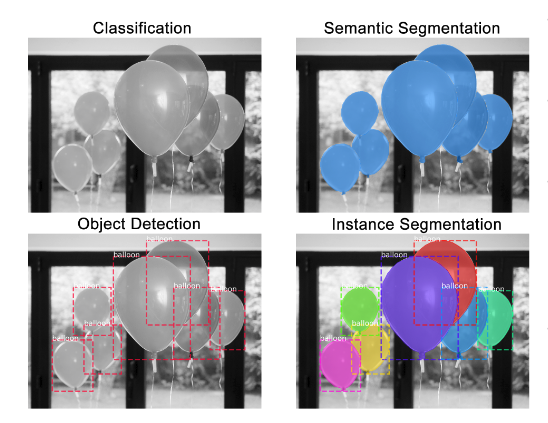
\includegraphics[width=12cm]{Bilder/applications.png} 
		\caption[Anwendungsgebiete von Deep Learning zur Bildverarbeitung im Überblick]{Anwendungsgebiete von Deep Learning zur Bildverarbeitung im Überblick \cite{PriyaDwivedi.20190328}}
		\label{applications}
	\end{center}
\end{figure}

Für eine einfache \textit{Klassifikation} eines Bildes können einfache sogenannte \textit{Feed-Forward} Netze verwendet werden. Es kann hierbei aber auch auf konventionelle Methoden der Bildverarbeitung zurück gegriffen werden. Für die \textit{Objektdetektion} stehen Architekturen wie \textit{You Only Loom Once} (YOLO), der \textit{Single Shot MultiBox Detector} (SSD) oder neuronale Netze der \textit{Regional Proposal Neural Networks} (R-CNN) bereit. Aus dieser Familie entstammt ebenso das \textit{Mask R-CNN} Netz, das zur \textit{Instanzbasierten Segmentierung} von Objekten verwendet wird.

\section{Problemstellung und Motivation}

Das \textit{Smart Warehouse} beschreibt ein Warenhaus, welches unter Einsatz einer Drohne in der Lage sei soll Inventuren und Bestandsprüfungen weitgehend ohne menschliche Hilfe durchzuführen. Das Live-Bild der Drohne soll von den Objektdetektoren dazu genutzt werden, Warengegenstände zu lokalisieren und klassifizieren. 

Neben der Frage, ob ein solches Industrieszenario überhaupt umsetzbar und wirtschaftlich sinnvoll ist, sollen die Objektdetektoren in diesem Anwendungsszenario nach verschiedenen Kriterien miteinander verglichen und beurteilt werden. Diese Kriterien lassen sich hauptsächlich in die Kategorien Präzision, Reaktionsvermögen und Trainingsverhalten untergliedern und werden später genauer eingeführt. Dadurch lassen sich Aussagen darüber treffen, ob nach dem momentanen Forschungsstand um Objektdetektoren solche das Potential bieten, industriell eingesetzt zu werden. 

Falls die Machbarkeitsstudie des \textit{Smart Warehouse} glückt, so kann der Industrie ein kostengünstiges, zeitsparendes und ressourcenschonendes Modell zur Inventurverwaltung eines Warenhauses angeboten werden.
\section{Vorgehensweise und Zielsetzung}

Im Grundlagenkapitel 2 muss sich mit den theoretischen Grundlagen von CNNs und Objektdetektoren auseinander gesetzt werden. Hierzu ist zunächst eine Einführung in Deep Learning zur Bildverarbeitung und neuronale Netz erforderlich, darunter zu Perzeptronen, dem Gradientenverfahren, dem Backpropagation Algorithmus und Hyperparametern zum Trainieren eines neuronalen Netzes (siehe Kapitel \ref{bildverarbeitung}, \ref{anns} und \ref{hyperparam}). 

Um weitere Grundlagen zum Training von neuronalen Netzen einzuführen, wird anschließend über die Anforderungen eines Datensatzes gesprochen (siehe Kapitel \ref{data}), bevor weitere Grundlagen zu Objektdetektoren eingeführt werden (siehe Kapitel \ref{basics}). 

Nachdem zu Beginn des Kapitels \ref{basics} kurz auf den Grundbaustein moderner Objektdetektoren eingegangen wird, den CNNs, können anschließend die Funktionsweisen und Architekturen der drei miteinander verglichenen Objektdetektoren der \textit{R-CNN} Familie, \textit{YOLO} und des \textit{SSDs} erläutert werden (siehe Kapitel \ref{detection}). Bei \textit{R-CNN} und \textit{YOLO} ist zu bemerken, dass unterschiedliche Evolutionsstufen der Detektoren zu betrachten sind.

Um weitere Grundlagen zum Training von neuronalen Netzen einzuführen, wird anschließend über zwei wesentlichen Speicherformate eines Datensatzes gesprochen (siehe Kapitel \ref{format}), bevor verschiedene Cloud Anbieter für das Trainieren von \textit{Deep Learning} Modellen aufgezeigt werden (siehe Kapitel \ref{cloud}). 

In Kapitel 3 werden chronologisch Teilziele der Konzeption beschrieben, darunter das Erstellen eines Trainingsdatensatzes (siehe Kapitel \ref{traindata}), dem Einführen von Bewertungskriterien (siehe Kapitel \ref{eval}), der Auswahl von Objektdetektoren, der Trainingsinfrastruktur und der Drohne (siehe Kapitel \ref{detect}, \ref{infrastructure}, \ref{drone_selection}) und die Spezifikation der Inventursoftware (siehe Kapitel \ref{software}).

In der Realisierung werden die Herausforderungen zur Steuerung und Anbindung der Drohne betrachtet und zudem die Objektdetektoren auf die realen Datensätze trainiert. Auch die Entwicklung der Webapplikation zur Visualisierung des Live-Bildes und der erkannten Objekte sowie der darin realisierte Zählalgorithmus zur Durchführung der Inventur wird Bestandteil dieses Kapitels sein. Die Ergebnisse der Realisierungsphase werden nach den in Unterkapitel \ref{eval} definierten Bewertungskriterien im folgenden Kapitel dargestellt. 

Ziel der Arbeit ist es Aussagen über die Fähigkeit von Objektdetektoren zum Einsatz in der Industrie zu treffen, indem eine Bewertung der Verhaltensweisen der Objektdetektoren nach den eingeführten Bewertungskriterien durchgeführt wird. Als Umgebung und Rahmenszenario für die Evaluation dient das \textit{SmartWarehouse} Szenario, dessen Machbarkeit ebenfalls herausgestellt werden soll (siehe Kapitel \ref{evaluation}).

Zuletzt wird das Wesen der Arbeit nochmals kurz zusammengefasst und anschließend auf mögliche Verbesserungen und Ausblicke in die Zukunft aufmerksam gemacht. 


\chapter{Grundlagen und Forschungsstand}

Neben einer Einführung in den Anwendungsbereich von \textit{Deep Learning} zur Bildverarbeitung soll sich das folgende Kapitel speziell mit Architekturen unterschiedlicher Objektdetektoren auseinander setzen und herausstellen, wie sich diese voneinander abgrenzen. Davor wird allerdings zunächst grundlegendes Wissen über neuronale Netze und wie diese \glqq lernen\grqq{} vermittelt sowie wie ein eigener Datensatz zu gestalten ist. Abschließend werden technische Grundlagen für die Programmierung des \textit{Smart Warehouse} Szenarios aufgezeigt.

\section{Deep Learning zur Bildverarbeitung}

Ein klassisches Anwendungsgebiet von \textit{Deep Learning} zu Bildverarbeitung oder auch allgemein von maschinellem Lernen beschreibt die \textit{Klassifikation}. Hierbei werden bestimmte Kategorien, auch \textit{Klassen} genannt, definiert, in die ein Bild eingeordnet werden soll. Die \textit{Klassifikation} wird anhand von aus dem Bild extrahierten Merkmalen, auch \textit{Features} genannt, getroffen. Die Merkmale werden zu einem \textit{Merkmalsvektor} oder auch \textit{Feature Map} zusammengefasst und von einem \textit{neuronalen Netz} verarbeitet. Das Ergebnis der Verarbeitung durch das neuronale Netz ist die Einordnung in eine bestimme Klasse. 

Zusätzlich zur \textit{Klassifikation} eines Bildes kann das auf dem Bild abgebildete Objekt ebenfalls lokalisiert werden. Es wird dann von sogenannter \textit{Objektdetektion} gesprochen. Es können auch mehrere Objekte auf einem Bild detektiert werden. Ergebnis der Objektdetektion ist somit nicht nur eine Klasseneinordnung sondern ebenso eine klare Positionsangabe des Objektes auf dem Bild. Die Positionsangabe erfolgt durch Angabe sogenannter \textit{Bounding Boxen}. Diese umrahmen das jeweils detektierte Objekt und werden durch ihren linken oberen Eckpunkt sowie ihre Höhe und Breite beschrieben. 

Neben der klassischen \textit{Klassifikation} und der \textit{Objektdetektion} existiert ebenso ein drittes Anwendungsgebiet von \textit{Deep Learning} zu Bildverarbeitung, die \textit{Segmentierung}. Bei der \textit{semantischen Segmentierung} wird versucht, jede einzelne Pixel eines Bildes einer Klasse zuzuordnen und dementsprechend farblich im Bild zu hinterlegen. \textit{Instanzbasierte Segmentierung} hingegen zielt darauf ab, nicht nur jeden Pixel zu einer Klasse zu klassifizieren, sondern ebenso eine Identität zu einem Objekt zuzuweisen \cite{RavindraParmar.20180902}. Es setzt sich zusammen aus \textit{semantischer Segmentierung} und paralleler \textit{Objektdetektion}.

Einen Überblick über die vorgestellten Anwendungsgebiete ist in Abbildung \ref{applications} zu sehen.

\begin{figure}[ht]
	\begin{center}
		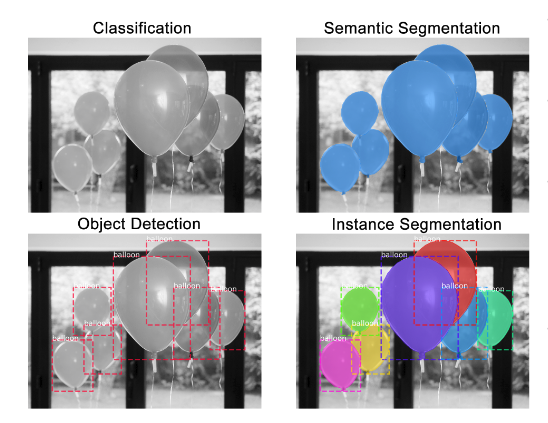
\includegraphics[width=12cm]{Bilder/applications.png} 
		\caption[Anwendungsgebiete von Deep Learning zur Bildverarbeitung im Überblick]{Anwendungsgebiete von Deep Learning zur Bildverarbeitung im Überblick \cite{PriyaDwivedi.20190328}}
		\label{applications}
	\end{center}
\end{figure}

Für eine einfache \textit{Klassifikation} eines Bildes können einfache sogenannte \textit{Feed-Forward} Netze verwendet werden. Es kann hierbei aber auch auf konventionelle Methoden der Bildverarbeitung zurück gegriffen werden. Für die \textit{Objektdetektion} stehen Architekturen wie \textit{You Only Loom Once} (YOLO), der \textit{Single Shot MultiBox Detector} (SSD) oder neuronale Netze der \textit{Regional Proposal Neural Networks} (R-CNN) bereit. Aus dieser Familie entstammt ebenso das \textit{Mask R-CNN} Netz, das zur \textit{Instanzbasierten Segmentierung} von Objekten verwendet wird.

\chapter{Grundlagen und Forschungsstand}

Im folgenden Kapitel soll sich speziell mit den Architekturen der unterschiedlichen Objektdetektoren auseinander gesetzt werden und wie sich diese voneinander abgrenzen. Außerdem wird grundlegendes Wissen über neuronale Netze und wie diese \glqq lernen\grqq{} vermittelt, um die späteren Optimierungsverfahren an den Objektdetektoren zu verstehen. Zuletzt werden technische Grundlagen für die Programmierung des \textit{Smart Warehouse} Szenarios vermittelt.

\section{Neuronale Netze}

Ein neuronales Netz bildet die Grundlage des \textit{Deep Learnings} \cite{AurelienGeron.2018}. Zunächst soll die einfachste Architektur eines neuronalen Netzes, das Perzeptron \cite{AurelienGeron.2018}, exemplarisch erklärt werden als auch der Lernprozess eines maschinellen Lernmodells an sich, um darauf basierend die Auswirkungen von Hyperparametern auf den Lernprozess des Modells zu erklären. 

\subsection*{Das Perzeptron}

Der Aufbau eines typischen Perzeptrons besteht aus einer oder mehreren Schichten sogenannter \textit{Linear Threshold Units} (LTU) wie in Abbildung \ref{ltu} dargestellt.

\begin{figure}[ht]
	\begin{center}
		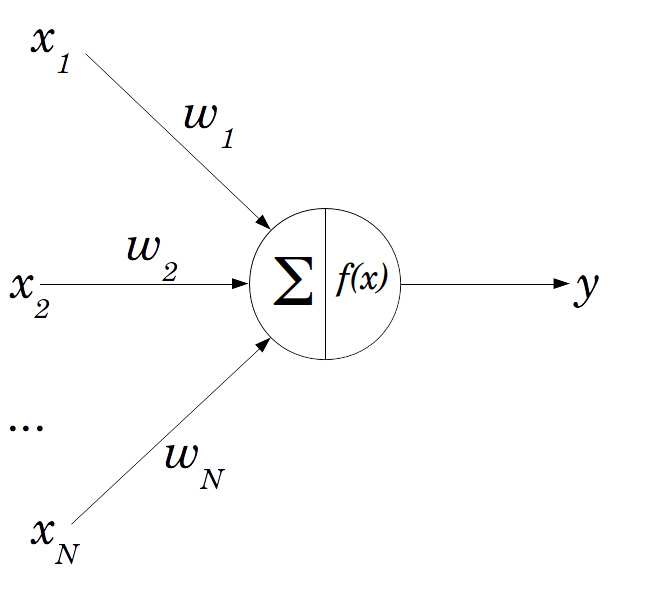
\includegraphics[width=9cm]{Bilder/perceptron.png} 
		\caption[Linear Threshold Unit]{Linear Threshold Unit \cite{PhilippeLucidarme.2017}}
		\label{ltu}
	\end{center}
\end{figure}

Es besteht aus $n$ Eingängen mit $x_{i} \in \mathbb{Q}$, die im Inputvektor $\boldsymbol{x}$ zusammengefasst werden. Jeder Eingang wird mit einem Gewicht $w_{i}$ aus dem Gewichtsvektor $\boldsymbol{w}$ versehen \cite{AurelienGeron.2018}. Die LTU berechnet das Skalarprodukt $\boldsymbol{w}^{T} \circ \boldsymbol{x}$ aller Eingänge $\boldsymbol{x}$ mit ihren Gewichten $\boldsymbol{w}$ und wendet anschließend auf das Ergebnis $z$ eine Aktivierungsfunktion an \cite{AurelienGeron.2018}. Das Ergebnis $h_{w}(x)$ kann anschließend als Eingabe für ein weiteres Perzeptron dienen. Die einfachste Aktivierungsfunkion für ANNs ist die \textit{Heaviside-Funktion} (\ref{heaviside}) \cite{AurelienGeron.2018}. Falls eine Klassifizierung mit Wahrscheinlichkeiten vorliegen soll, so ist die letzte Schicht eines Perzeptrons meist mit der \textit{Softmax-Funktion} (\ref{softmax}) implementiert, die den Wert des $j$-ten LTUs einer Schicht mit allen anderen $n$ Werten der LTUs derselben Schicht ins Verhältnis setzt \cite{AurelienGeron.2018}. Es gibt eine Vielzahl an möglichen Aktivierungsfunktionen, die im darauffolgenden Unterkapitel \textit{Hyperparameter} betrachtet werden.

\begin{equation} \label{heaviside}
\begin{split}
h_{w}(x) = s(\boldsymbol{w}^{T} \circ \boldsymbol{x}) = s(z) = \\\ \begin{pmatrix} 
w_{1}&&w_{2}&&\dots&& w_{n}\\ 
\end{pmatrix} 
\circ 
\begin{pmatrix} x_{1}\\
x_{2}\\
\vdots\\
x_{n}\\
\end{pmatrix}) = 
\begin{cases}
1 & \text{wenn} z \geq 0 \\
0 & \text{wenn} z < 0 \\
\end{cases}
\end{split}
\end{equation}
\equations{Die Heaviside-Funktion}

\begin{equation} \label{softmax}
h_{w}(x) = \sigma(z)_j = \frac{e^{z_j}}{\sum_{i=0}^n e^{z_i} }
\end{equation}
\equations{Die Softmax-Funktion}

Die Aktivierung einer LTU hängt zusätzlich von einem Schwellwert $\theta$ ab, der durch einen sogenannten \textit{Bias} festgelegt wird. Dies ist die Gewichtung des letzten Eingangs, der standardmäßig den Wert 1 liefert. Wählt man die Gewichtung negativ, so ist es schwieriger die LTU zu aktivieren, während eine positive Gewichtung die Aktivierung vereinfacht \cite{AurelienGeron.2018}.

Nun bilden ein oder mehrere Schichten solcher LTUs ein Perzeptron. Jede einzelne LTU ist dabei mit allen LTUs der vorherigen Schicht verbunden (siehe Abbildung \ref{neural_network}) \cite{AurelienGeron.2018}. Die beiden LTUs zur Ausgabe können dabei Aussagen über eine Klassifikation von Daten anhand der Eingangsdaten treffen, während die LTUs im Input Layer wesentlich die Daten weiter reichen. Die Verbindungen zur ersten Schicht des Hidden Layer sind stets mit Eins belegt. Existiert keine verborgene Schicht, so bezeichnet man das ANN als einschichtiges Perzeptron, ab einer oder mehr verborgenen Schichten spricht man bereits von einem \textit{Multi-Layer Perzeptron} (MLP), einem mehrschichtigen Perzeptron \cite{AurelienGeron.2018}. Ist das neuronale Netz optimal trainiert, so ist am Ende nur eines der LTUs zur Ausgabe aktiviert. Das folgende ANN ist zudem ein Beispiel für ein sogenanntes \textit{Feed Forward Network}, bei dem die Auswertung der Daten von einer Schicht zur nächsten weitergereicht wird, ohne zu bereits besuchten Schichte zurückzukehren \cite{AurelienGeron.2018}.

\begin{figure}[ht]
	\begin{center}
		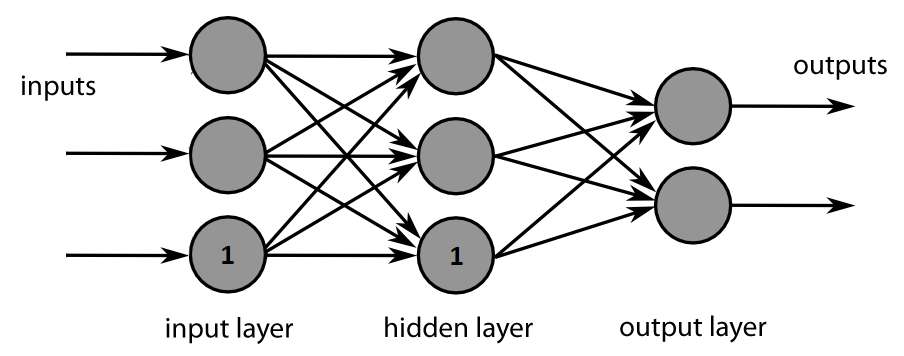
\includegraphics[width=12cm]{Bilder/neural_network.png} 
		\caption[Das einschichtige Perzeptron]{Das einschichtige Perzeptron \cite{Wikipedia.20190123}}
		\label{neural_network}
	\end{center}
\end{figure}

\subsection*{Gradientenverfahren und Backpropagation}

Um zu verstehen, wie ein neuronales Netz durch Training lernt, muss zunächst der Begriff der Kostenfunktion (engl.: cost function) eingeführt werden. Die Kostenfunktion ist ein Qualitätsmaß dafür, wie weit die Ausgabe einer LTU vom erwarteten Wert abweicht \cite{AurelienGeron.2018}. Angenommen dem neuronalen Netz wird ein Datensatz zur Klassifikation übergeben, so ist am Ende meist nicht nur eine LTU zu Ausgabe aktiviert, was auf eine eindeutige Klassifikation schließen würde, sondern meist mehrere zu einem frühen Stadium des neuronalen Netzes.

Eine oft genutzte Kostenfunktion ist die \textit{Root Mean Squared Error Funktion} (RMSE) (\ref{mse}) \cite{AurelienGeron.2018}

\begin{equation} \label{mse}
E(\boldsymbol{z},\boldsymbol{o}) = \sqrt{\frac{1}{n}\sum_{k=0}^n \lVert{z_k-o_k}\rVert^2} = \sqrt{\frac{1}{n}\sum_{k=0}^n (z_k-o_k)^2}.
\end{equation}
\equations{Die RMSE-Funktion}

Hierbei ist $z$ der erwartete Ausgabevektor des Perzeptrons, während $o$ die momentane Ausgabe darstellt. Da der erwartete Ausgabewert bekannt ist, spricht man auch von sogenanntem überwachtem Lernen \cite{AurelienGeron.2018}. Den Fehler der Abweichung dieser beiden Werte gilt es nun schrittweise zu minimieren. Um dies zu erreichen können die drei Parameter

\begin{enumerate}
	\item Gewichtung der Verbindungen zum Perzeptron
	\item Bias zur Aktivierung der LTUs des Perzeptrons und
	\item Stärke der Aktivierung des vorherigen Perzeptrons
\end{enumerate}

angepasst werden \cite{AurelienGeron.2018}. Hierbei wird das sogenannte \textit{Gradientenverfahren} eingesetzt. Es berechnet in einem iterativen Prozess über mehrere Testdaten das globale Minimum der Kostenfunktion nach den Gewichtungen der Verbindungen und damit auch nach den Bias Werten, die natürlich ebenso Gewichtungen darstellen. Ergebnis eines Durchlaufs im Gradientenverfahren (\ref{gradientenverfahren}) ist die Gewichtungsmatrix, die die Änderung der Gewichtung jeder einzelnen Verbindung eines Perzeptrons zu jeder LTU des Folgeperzeptrons angibt \cite{AurelienGeron.2018}.

\begin{equation} \label{gradientenverfahren}
w_{ijt} = w_{ijt-1} - \eta\frac{\partial E}{\partial w_{ij}} \qquad\text{\cite{PhilippeLucidarme.2017}} 
\end{equation}
\equations{Neuberechnung der Gewichtungsmatrix durch partielle Differentiation}

Das Gradientenverfahren eignet sich allerdings nur für stetig differenzierbare Funktionen ohne Plateaus. Somit können beispielsweise bei der Heaviside-Funktion als Aktivierungsfunktion Probleme auftreten, da eine Ableitung der Kostenfunktion stets Null betragen würde, wohingegen bei der später eingeführten Sigmoid-Funktion im gesamten Definitionsbereich immer kleine Änderung der Gewichtungen zu verzeichnen wären \cite{AurelienGeron.2018}.

Nun stellt sich auch der Vorteil von MSE als Kostenfunktion gegenüber anderen, durchaus komplexeren Kostenfunktionen heraus. Während MSE genau ein Minimum, das zugleich das globale Minimum der Funktion darstellt, besitzt, haben andere Kostenfunktionen im Gradientenverfahren das Problem, dass anstelle des globalen Minimums auch nur lokale Minima erreicht werden können \cite{AurelienGeron.2018}. Dies hat zur Folge, dass mehrere iterative Durchlaufe mit mehreren Testdatensätzen nötig werden, um durch unterschiedliche Startkonfigurationen die unterschiedlichen Minima miteinander vergleichen zu können und damit das globale Minimum herauszustellen.

Durch das Gradientenverfahren werden somit nur diejenigen Verbindungen verstärkt, die zum richtigen Ergebnis führen. 

Nun bleibt nur noch die dritte Möglichkeit zur Minimierung der Kostenfunktion übrig, die Anpassung der Stärke der Aktivierung des vorherigen Perzeptrons. Zu diesem Problem veröffentlichten David E. Rumelhart, Geoffrey E. Hinton und Ronald J. Williams 1985 den sogenannten \textit{Backpropagation-Algorithmus} \cite{DavidE.Rumelhart.September1985}. Dieser berechnet mit Hilfe des Gradientenverfahren welchen Anteil am Fehler der Ausgabe jede LTU des letzten Perzeptrons hat und anschließend welcher Anteil davon wiederum auf das vorherige Perzeptron der vergorenen Schicht zurück zu führen ist. Das Gradientenverfahren wird solange wiederholt, bis die Eingangsschicht erreicht wurde, es berechnet also für jede LTU deren Anteil am Fehler des Ergebnisses \cite{AurelienGeron.2018}.

Mit Hilfe des Gradientenverfahren im Backpropagation Algorithmus wird nun also das neuronale Netz durch mehrere iterative Durchläufe trainiert, wobei das Training als Anpassung der Gewichtungen einzelner Verbindungen zu verstehen ist.
\section{Hyperparameter}

Als Hyperparameter versteht man die Parameter, die zur anfänglichen Konfiguration des neuronalen Netzes als auch zur Konfiguration des Lernprozesses heran gezogen werden. Um im Laufe der Arbeit verstehen zu können, wie die Objektdetektoren auf Seiten der Netzarchitektur und des Lernverhaltens optimiert wurden, ist demnach ein kurzer Einblick in den Themenbereich der Hyperparameter von Nöten.

\subsection*{Anzahl der LTUs}
Die Anzahl der LTUs im ANN ist dafür ausschlaggebend, wie hoch der Komplexitätsanspruch eines Klassifizierungsproblems sein darf, um noch vom ANN gelöst werden zu können. Die Anzahl der LTUs hängt hauptsächlich von den Eingangsdaten ab. Über die optimalste Anzahl an LTUs pro Schicht lässt sich allerdings nur schwer etwas vorhersagen. Generell gilt, dass bei gleicher Anzahl an LTUs tiefere Netze eine weitaus höheren Parametereffizienz aufweisen als breitere Netze, da diese schneller gegen den gewünschten Zustand konvergieren. Zudem lassen sie sich somit schneller und kostengünstiger trainieren. So müssten bei einem 2x32 Netz 1024 Gewichtungen angepasst werden, während es bei einem 32x2 Netz dies nur 128 sind.  \cite[S. 271 f.]{AurelienGeron.2018}

\subsection*{Initialisierung der Gewichtungen}
Auch stellt die Initialisierung der Gewichte eines ANNs zu Beginn des Trainingsprozesses eine berechtigte Frage dar. Falls keine bereits trainierten ANNs für ein Klassifikationsproblem vorliegen, so werden die Gewichtungen meist zufällig nach einer Normalverteilung gewählt \cite[S. 271]{AurelienGeron.2018}. 

Dies hat allerdings zur Folge, dass nach der Berechnung der gewichteten Summen aller LTUs die Werte der folgenden Schicht nicht mehr normalverteilt sind, da für die Varianz das Superpositionsprinzip gilt (siehe Formel \ref{varianz})

\begin{equation} \label{varianz}
Var(X + Y) = VAR(X) + VAR(Y)
\end{equation}
\equations{Superpositionsprinzip anhand der Varianz}

\begin{equation} \label{xavier}
W \sim U[-\frac{\sqrt{6}}{\sqrt{n_{j} + n_{j+1}}},\frac{\sqrt{6}}{\sqrt{n_{j} + n_{j+1}}}]
\end{equation}
\equations{Standardverteilung nach Xavier Initialisierung}

Durch die größer werdende Standardabweichung können demnach Werte entstehen, die weit über den Mittelwert von Null hinaus gehen. Dies kann wiederum dazu führen, dass der Gradientenabstieg während des Backpropagation-Verfahrens nur langsam vollzogen werden kann, da der Gradient bei bestimmten Aktivierungsfunktionen (siehe Abbildung \ref{sigmoid}) gegen Null konvergiert \cite[S. 275 f.]{AurelienGeron.2018}. 

Eine \textit{Xavier Initialisierung} umgeht das Problem der sogenannten \textit{schwindenden Gradienten}, indem die Gewichte nach \ref{xavier} gleichverteilt werden, wobei $n{j}$ die Anzahl an LTUs der $j-ten$ Schicht sind. \cite[S. 253]{XavierGlorot.2010}

\subsection*{Auswahl des Gradientenverfahrens}

Generell unterscheidet man zwischen drei verschiedenen Arten das Gradientenverfahren durchzuführen (siehe Abbildung \ref{gradient}):

\begin{figure}[ht]
	\begin{center}
		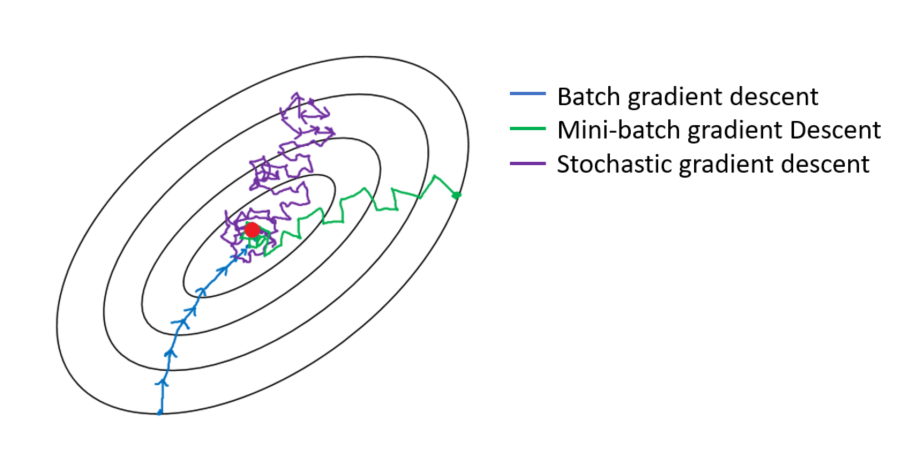
\includegraphics[width=15cm]{Bilder/gradient_descent.png} 
		\caption[Gradientenverfahren]{Gradientenverfahren \cite{ImadDabbura.20171221}}
		\label{gradient}
	\end{center}
\end{figure}

Beim \textit{Batch} Verfahren werden in einem Trainingsdurchlauf, auch \textit{Epoche} genannt, alle vorhandenen Daten des Trainingsdatensatzes herangezogen, um einen Gradientenabstieg zu vollziehen. Dies ist bei großen Trainingsdatensätzen auffällig langsam, dafür aber hinsichtlich der Erreichung des lokalen Minimums sehr zielstrebig. \cite[S. 116]{AurelienGeron.2018}

Das \textit{stochastische Gradientenverfahren} führt nach jedem einzelnen Dateneintrag im Trainingsdatensatz einen Gradientenabstieg durch. Da nur wenige Daten des ANNs verändert werden müssen, ist dieses Verfahren deutlich schneller, dafür aber unregelmäßiger hinsichtlich der Erreichung des Minimums. Oft wird das stochastische Gradientenverfahren verwendet, wenn nicht der komplette Trainingsdatensatz in den Hauptspeicher oder Grafikspeicher geladen werden kann. Diese Fähigkeit wird oft als \textit{Out-of-Core} Fähigkeit bezeichnet. Es hat auch den Vorteil, besser das globale Minimum der Kostenfunktion aufzufinden, da bei lokalen Minima die Chance besteht, durch den unregelmäßigen Gradientenabstieg das lokale Mimima wieder zu überwinden. \cite[S. 118 f.]{AurelienGeron.2018}

Ein Kompromiss der beiden Verfahren bietet das \textit{Mini-Batch} Verfahren, bei dem wiederholt Teilmengen des gesamten Datensatzes für einen Gradientenabstieg verwendet werden. Genauso wie das \textit{Batch} Verfahren bietet das \textit{Mini-Batch} Verfahren den Vorteil, die partiellen Ableitungen als Matrizenoperationen auf die Grafikkarten auszulagern, um die Performanz durch Parallelisierung zu steigern. \cite[S. 121]{AurelienGeron.2018}

\subsection*{Lernrate}

Die Lernrate $\eta$ gibt an, wie groß die Sprünge zum globalen Minimum sein sollen und damit indirekt wie viele Iterationen benötigt werden, um das globale Minimum der Kostenfunktion zu erreichen. Ziel der Anpassung einer Lernrate ist es, mit möglichst wenig Iterationen und Testdaten die optimale Konstellation des neuronalen Netzes zu berechnen. Deshalb wird sie standardmäßig zu Beginn der Iterationen groß gewählt um sich dem Minimum schnell zu nähern während sie am Ende immer kleiner gewählt wird, um nicht über das globale Minimum hinaus zu gehen. Dieses Vorgehen wird als \textit{Simulated Annealing} bezeichnet, während das Funktion zum Festlegen der Lernrate als \textit{Learning Schedule} betitelt wird. \cite[S. 113f]{AurelienGeron.2018}

Eine Veranschaulichung der Anpassungen der Lernrate findet sich in Abbildung \ref{learning_rate}.

\begin{figure}[ht]
	\begin{center}
		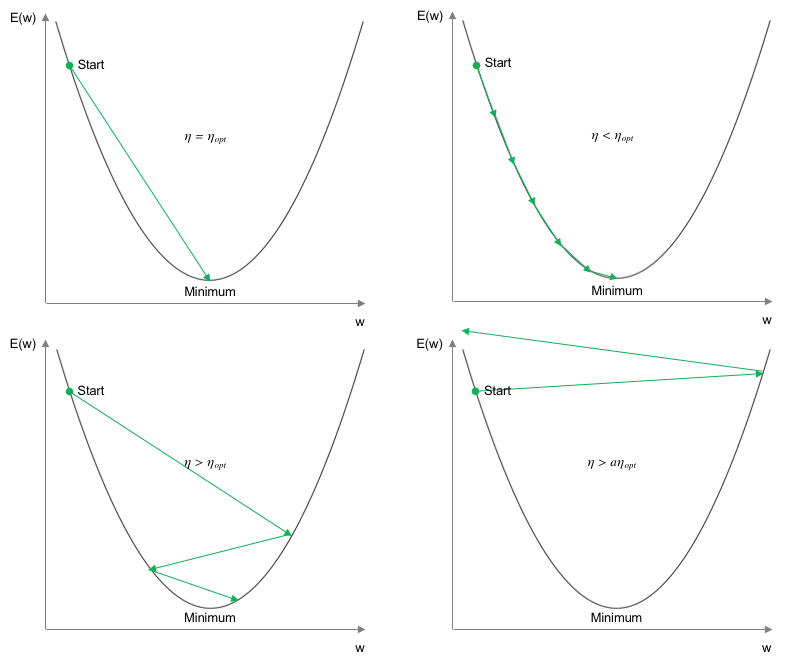
\includegraphics[width=11cm]{Bilder/learning_rate.png} 
		\caption[Auswirkung unterschiedlicher Lernraten]{Auswirkung unterschiedlicher Lernraten \cite{SebastianHeinz.2018}}
		\label{learning_rate}
	\end{center}
\end{figure}

Die Anzahl der Durchläufe wird zu Beginn des Verfahrens zunächst hoch angesetzt, das Verfahren wird aber genau dann gestoppt, sobald der Gradientenvektor unter eine gewisse Abbruchgrenze fällt. Zwar ist das globale Minimum zu diesem Zeitpunkt noch nicht erreicht, allerdings kann es auch nie vollkommen erreicht werden, da die für das Gradientenverfahren genutzten Aktivierungsfunktionen nie einen partiellen Ableitungswert gleich Null zulassen \cite[S. 118, S. 272]{AurelienGeron.2018}. In diesem Sinne wird auch von \textit{Toleranz} gesprochen.

\subsection*{Anzahl an Epochen}

Die Anzahl der Epochen beschreibt die Durchläufe durch einen bestimmten Trainingsdatensatz während der Trainingsphase. Ist die Anzahl zu hoch gewählt wird Gefahr gelaufen sogenanntes \textit{Overfitting} des ANNs zu erreichen. Dies bedeutet ein fehlendes Abstraktionsvermögen des ANNs zu erreichen und damit alleinig eine richtige Erkennung der Trainingsdatensätze zu ermöglichen.  

\subsection*{Aktivierungsfunktionen}

Zwei bekannte und ähnliche Aktivierungsfunktionen sind die \textit{Sigmoid-Funktion} und die \textit{Tangens Hyperbolicus} Funktion (siehe Abbildung \ref{sigmoid}).

\begin{figure}[ht]
	\begin{center}
		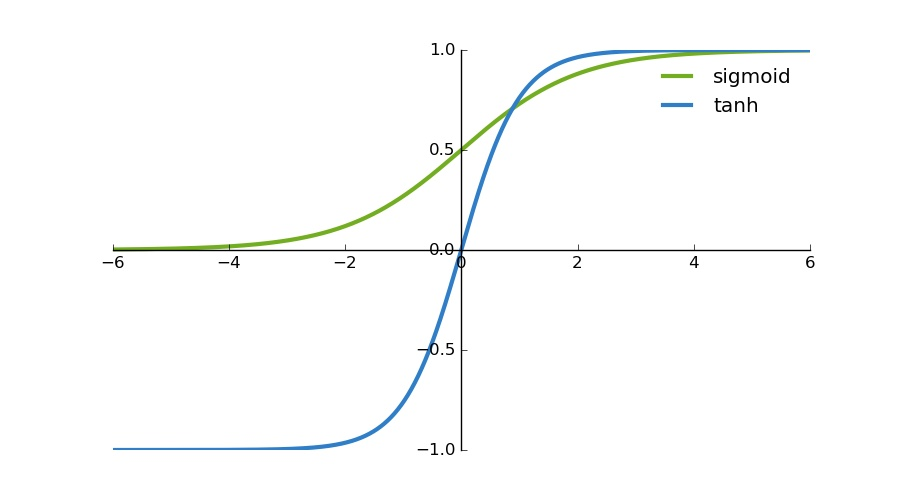
\includegraphics[width=15cm]{Bilder/sigmoid.jpg} 
		\caption[Sigmoid und Tangens Hyperbolicus]{Sigmoid und Tangens Hyperbolicus \cite{RonnyRestrepo.20170816}}
		\label{sigmoid}
	\end{center}
\end{figure}

Da diese allerdings anfällig für das Problem \textit{schwindender Gradienten} sind \cite[S. 276]{AurelienGeron.2018}, wird die \textit{Rectified Linear Unit} (ReLU) bzw. \textit{Parametric/Leaky Rectified Linear Unit} (PReLU/LRelU) Aktivierungsfunktion bevorzugt (siehe Abbildung \ref{relu}). 

\begin{figure}[ht]
	\subfigure[RELU]{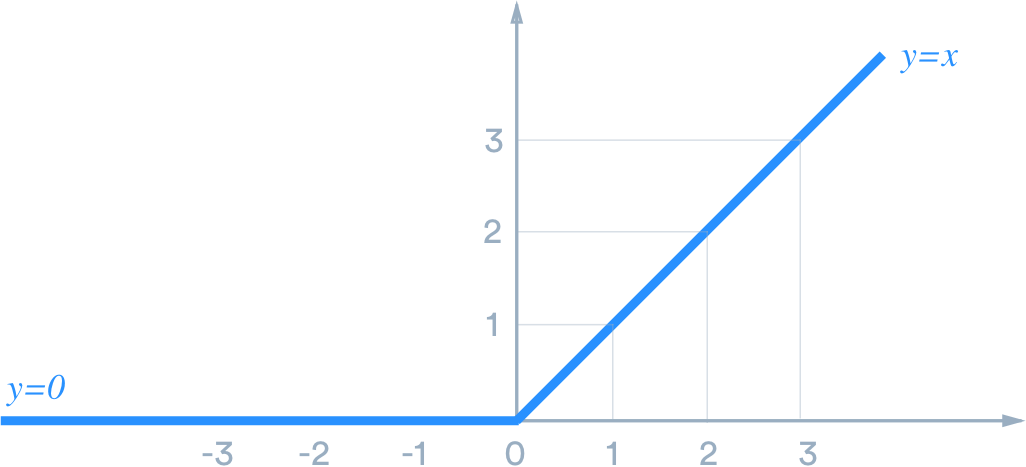
\includegraphics[width=7.5cm]{Bilder/relu.png}} 
	\subfigure[PReLU/LReLU]{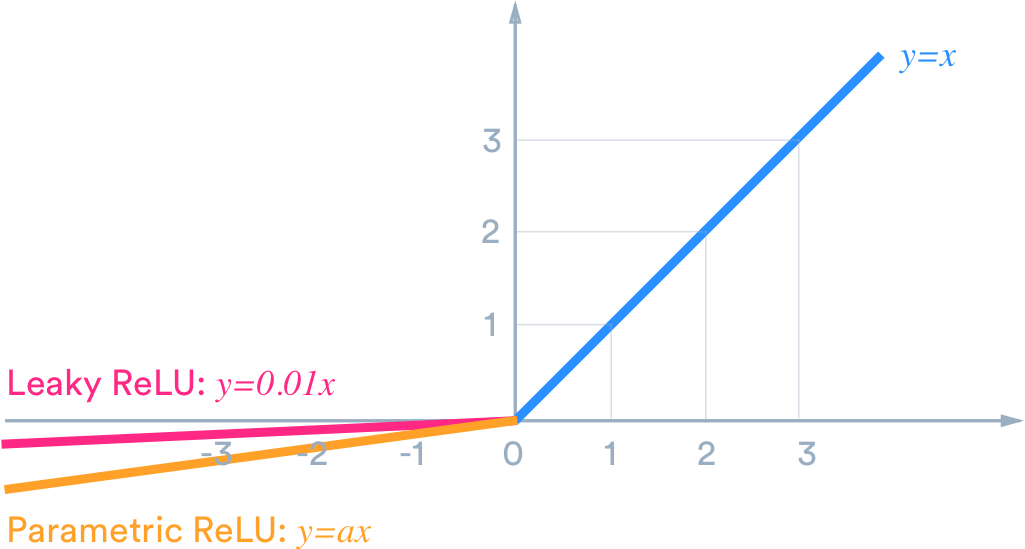
\includegraphics[width=7.5cm]{Bilder/prelu.png}} 
	\caption[ReLU-Aktivierungsfunktionen]{ReLU-Aktivierungsfunktionen \cite{DanqingLiu.20171130}} 
	\label{relu}
\end{figure} 

Bei ReLU kann es während des Trainingsprozesses dazu kommen, dass LTUs nach dem Gradientenabstieg einen negativen Wert aufweisen, weshalb sie nicht weiter aktiviert werden und für den Rest der Trainingsdauer \glqq tot\grqq{} sind. Um dies zu verhindern wurde \textit{LReLU} dazu genutzt, um eine Reaktivierung zu ermöglichen, da auch für negative LTU Werte ein Gradient der Aktivierungsfunktion bestimmt werden kann. Bei \textit{LReLU} ist die Steigung der Funktion im zweiten Quadranten statisch gewählt, während sie bei \textit{PReLU} dynamisch von neuronalen Netz während des Trainingsprozesses selbst gelernt werden kann. \cite[S. 280 f.]{AurelienGeron.2018}

Eine letzte Variante der Aktivierungsfunktionen beschreibt die \textit{ELU} Funktion (siehe Abbildung \ref{elu}).

\begin{figure}[ht]
	\begin{center}
		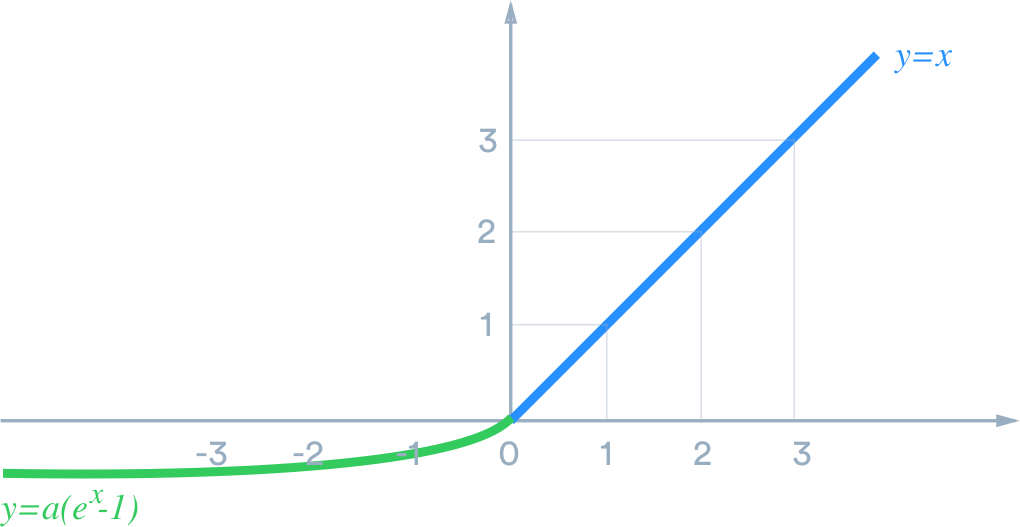
\includegraphics[width=15cm]{Bilder/elu.png} 
		\caption[ELU]{ELU \cite{DanqingLiu.20171130}}
		\label{elu}
	\end{center}
\end{figure}

Sie besitzt nicht nur die Eigenschaft schwindende Gradienten und tote LTUs zu verhindern, sondern ist im gesamten Definitionsbereich ebenso eine stetig differenzierbare Funktion, was das Gradientenverfahren beschleunigt. Als Standardwert für $\alpha$ wird oft Eins verwendet. Nachteil der \textit{ELU} Funktion ist der erhöhte Rechenaufwand, was aber durch die schnellere Konvergenz kompensiert wird. \cite[S. 280 f.]{AurelienGeron.2018}

\section{Datensatzlehre}

\subsection{Datensatzformate}

Basierend darauf welcher Objektdetektor trainiert werden soll, muss der zum Training verwendete Datensatz in einem bestimmten Format vorliegen. Zum Trainieren des \textit{SSDs} wird das sogenannte \textit{Pascal Visual Object Classes} (PascalVOC) Format benötigt. 

Es definiert eine Unterteilung in \textit{Annotations}, \textit{ImageSets} und \textit{JPEGImages}. Während in dem Ordner \textit{JPEGImages} alle Bilder des Datensatzes vorhanden sind, befindet sich unter anderem die Information über die vorhandenen Objekte in dem Bild im Ordner \textit{Annotations}. Für jedes Bild des Datensatzes werden die Informationen in einer gleichnamigen XML-Datei abgelegt. 

\lstset{language=XML}
\lstinputlisting[
label=pascalvoc:PascalVOC,
caption=pascalVOC Bildannotation,
captionpos=b,
firstline=1,
lastline=26
]{Quellcode/annotation.xml}

Neben allgemeinen Metainformationen über das Bild befindet sich hier ebenso eine Liste aller markierten Objekte. Pro Objekt wird die Klassifikationskategorie, die Ausrichtung (z.B. \glqq Frontal\grqq{}), die Information über vollständiges Erscheinen im Bild, die Information über schwere Erkennbarkeit und die Bounding Box angegeben. Im Ordner \textit{ImageSets/Main} wird eine Unterteilung in Trainings- und Testdatensatz durch zwei Textdateien realisiert, die die Dateinamen der Bilddateien als Auflistung enthalten. \cite{RenuKhandelwal.2019}

Das \textit{YOLO} Format für den \textit{YOLO} Objektdetektor definiert in einer \textit{.names}-Datei alle im Datensatz vorhandenen Kategorien durch simple Auflistung der Bezeichner. Die Bilder werden zusammen mit ihren Annotationen in einem separaten Ordner abgelegt. Die Annotationen folgen hier dem Format:

$<Kategorie-ID>\:<Zentrum-X>\:<Zentrum-Y>\:<Breite>\:<Hoehe>$

Die Unterteilung in Trainings- und Testdatensatz erfolgt durch Referenzierung der Bildpfade in zwei getrennten Textdateien. Schließlich wird in einer \textit{.data}-Datei der Pfad zu den beiden Textdateien und zur \textit{.names}-Datei sowie die Anzahl an Kategorien gespeichert. \cite{ArunPonnusamy.20191006}

\subsection{Datensatzzusammensetzung}

Zum Erstellen und Auswählen eines \textit{Deep Learning} Modells wird der Datenbestand in der Regel in drei Kategorien unterteilt. Ein Datensatz wird für das Training des Modells verwendet. Durch das anschließende Anwenden des Modells auf zuvor ungesehene Daten, den Testdaten, wird der \textit{Verallgemeinerungsfehler} gemessen, der möglichst niedrig ausfallen sollte. Fällt der allgemeine Fehler während des Trainings niedrig aus, der \textit{Verallgemeinerungsfehler} während des Testdurchlaufs allerdings hoch, so liegt klassisches \textit{Overfitting} vor, die Trainingsdaten wurden auswendig gelernt. \cite{AurelienGeron.2018}

Anschließend werden in mehreren Durchläufen die Hyperparameter des Trainingsprozesses angepasst, sodass letztendlich der \textit{Verallgemeinerungsfehler} für die Testdaten niedrig ausfällt. Kommt es anschließend zum Einsatz des Modells in der Produktivumgebung, so können trotz allem unerwartete Ergebnisse bezüglich des Abstraktionsvermögens des Modells auftreten. Dies liegt daran, dass das Modell allein auf die Testdaten hin optimiert wurde. Um dies zu vermeiden wird ein dritter Datensatz, der Validierungsdatensatz, eingeführt. Mehrere Modelle werden dabei durch den Validierungsdatensatz getestet und das dabei am besten abschneidende Modell mit dessen Hyperparametern ausgewählt. Der eigentliche Testdatendatz wird anschließend nur noch zur Abschätzung des \textit{Verallgemeinerungsfehlers} verwendet. \cite{AurelienGeron.2018}

Oft wird der Trainingsdatensatz mit dem Validierungsdatensatz zum sogenannten \textit{Trainval} Datensatz zusammengeführt. Dies steht im Kontext des sogenannten \textit{K-Kreuzvalidierungsverfahrens}. Dabei wird der \textit{Trainval} Datensatz in K gleich große, komplementäre Untermengen unterteilt. Eine dieser Untermengen dient anschließend als Validierungsdatensatz. Für jedes zu trainierende Modell mit unterschiedlichen Hyperparametern wird eine andere Untermenge als Validierungsdatensatz ausgewählt. Hierdurch steigt die Aussagekraft des Abstraktionsvermögens nach der Validierung und zudem müssen keine Trainingsdaten dauerhaft für die Validierung zurück gelegt werden. In der Regel werden 80\% der Gesamtdaten als \textit{Trainval} Datensatz verwendet. \cite{AurelienGeron.2018}

\subsection{Qualität und Quantität der Daten}

Um ein funktionsfähiges Modell zu trainieren muss der Datensatz einem gewissen Standard nachkommen. Demnach müssen die zu klassifizierenden Objekte vollständig im Bild enthalten und gut erkennbar sein. Zwar gibt es gerade im \textit{PascalVOC} Datensatzformat ebenso die Möglichkeit Objekte als \glqq schwierig erkennbar\grqq{} zu markieren, dennoch sollten solche Objekte nicht die Mehrheit im gesamten Datensatz ausmachen. Auch die Aufnahme von Objekten in unterschiedlichen Umgebungen, Entfernungen und Blicklagen fördert langfristig das Abstraktionsvermögen des Modells. 

Ebenso muss ein ausreichend großer Datensatz vorliegen, um das gewünschte Abstraktionsvermögen des Modells zu erreichen. Die Ergebnisse aus \ref{result} wurden beispielsweise durch Kombination der \textit{Trainval} Datensätze von PascalVOC 2007 und 2012 erzielt und umfasst 16.551 Bilder im Trainingsverfahren. \cite{ssd.20161229} \cite{MarkEveringham.20070607} \cite{MarkEveringham.20120521}

\begin{figure}[ht]
	\begin{center}
		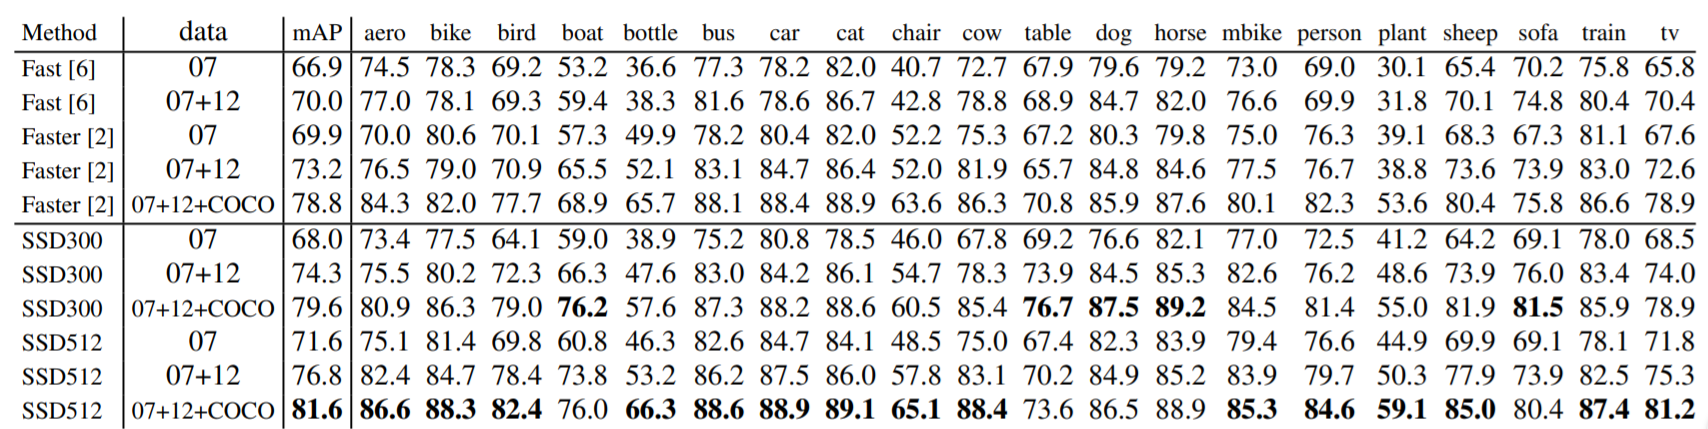
\includegraphics[width=15cm]{Bilder/ssd_results_details.png} 
		\caption[SSD Grundprinzip]{SSD Grundprinzip \cite{ssd.20161229}}
		\label{amountofdata}
	\end{center}
\end{figure}

Unter Hinzunahme des COCO \textit{trainval135k} Datensatzes erreicht der \textit{SSD} sogar das beste Ergebnis aus der ursprünglichen Veröffentlichung (siehe Abbildung \ref{amountofdata}) \cite{ssd.20161229}. 

\subsection{Techniken zur Verbesserung von Trainingsergebnissen}

Datenaugmentierung und Transfer-Learning

\section{Objektdetektoren}

\subsection{Convolutional Neural Networks}

Ein CNN besteht aus zwei grundlegenden Bausteinen, den sogenannten \textit{Convolutional Layern} und \textit{Pooling Layern}.

Ein Convolutional Layer zeichnen sich unter anderem dadurch aus, dass jede LTU dieser Schicht nicht mit allen vorherigen LTUs der vorgegangenen Schicht verbunden ist, sondern nur mit einer festen, beschränkten Anzahl. Es ist also kein vollständig verbundenes neuronales Netz. Dies macht es möglich, dass auch große Bilder klassifiziert werden können, ohne dass die Anzahl an nötigen Verbindungen im ANN unüberschaubar groß wächst. Die folgenden LTUs der zweiten Schicht sind ebenfalls wiederum nur mit einem Ausschnitt vorangegangener Neuronen verbunden und fassen die erkannten, kleinteiligen Merkmale der ersten Schicht zu übergeordneten, zusammengesetzten und komplexeren Merkmalen zusammen. \cite[S. 361]{AurelienGeron.2018}

Um allerdings Convolutional Layer genauer zu verstehen, ist anstelle einer eindimensionalen Darstellung eines Layers eine dreidimensionale Darstellung besser geeignet.

Zunächst kann ein zweidimensionale Bild als Matrix dargestellt werden, bei der jedes Element der Matrix den Grauwert eines Pixels zwischen 0 und 255 trägt. Die dadurch entstandene zweidimensionale Schicht bildet den Input-Layer mit einer LTU pro Pixel. Anschließend werden auf diese Schicht mehrere Filter angewandt, die die Gewichte des CNNs tragen und Muster aus dem Bild extrahieren. Die Stellen, die dem Muster ähnlich sind werden verstärkt, während Stellen, die nicht dem Muster entsprechen durch eine Nullgewichtung ausgelöscht werden. In Abbildung \ref{convolutional_layer} ist ein 3x3 Pixel Filter mit dessen Anwendung dargestellt. Ein Filter besitzt die Größe des künstlichen Wahrnehmungsfeldes einer LTU. \cite[S. 362 f.]{AurelienGeron.2018}

\begin{figure}[ht]
	\begin{center}
		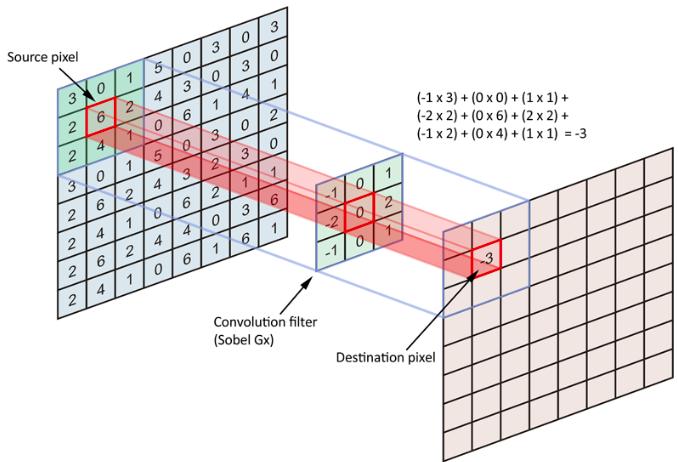
\includegraphics[width=12cm]{Bilder/convolutional_layer.png} 
		\caption[Convolutional Layer]{Convolutional Layer \cite{DaphneCornelisse.20180424}}
		\label{convolutional_layer}
	\end{center}
\end{figure}

Ein Filter wird dazu verwendet, jeden Pixel der Eingabeschicht auf die folgende Schicht abzubilden. Um keine Informationen zu verlieren und den Filter ebenso auf Randbereich anwendbar zu machen, wird oft ein sogenanntes \textit{Zero-Padding} auf eine Schicht angewandt, bei dem die Randbereiche mit LTUs des Wertes 0 aufgefüllt werden (siehe Abbildung \ref{zero_padding}). \cite[S. 362]{AurelienGeron.2018}

\begin{figure}[ht]
	\begin{center}
		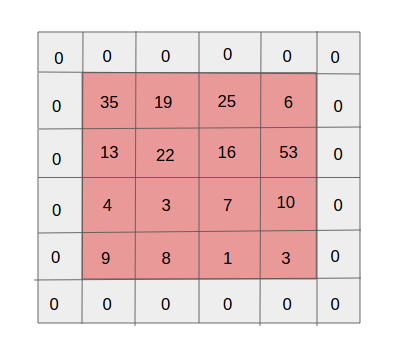
\includegraphics[width=7cm]{Bilder/zero_padding.png} 
		\caption[Zero-Padding]{Zero-Padding \cite{AbhineetSaxena.20160629}}
		\label{zero_padding}
	\end{center}
\end{figure}

Falls eine gleich große folgende Schicht gewünscht ist, wird eine Schrittweite (engl.: \textit{stride}) von 1 gewählt. Dies dient vor allem dazu kleinere Strukturen noch zu erkennen. Der Filter wird von einem Pixel zum direkt benachbarten Pixel bewegt und angewandt. In tieferen, fortgeschritteneren Schichten kann die Schrittweite auch größer als 1 gewählt werden, da hier bereits nach dem Anwenden mehrerer Filter feinere Muster erkannt wurden und diese nun zu größeren zusammengesetzt werden. Dabei verkleinert sich die resultierende Schicht. \cite[S. 362 f.]{AurelienGeron.2018}

Das Ergebnis der Anwendung eines Filters wird als \textit{Feature-Map} bezeichnet. Da mehrere Filter auf die gleiche Schicht angewandt werden, entstehen ebenso mehrere Feature Maps der Schicht. Stellt man sich diese Feature Maps übereinander gelagert vor, so entsteht der dreidimensionale, \glqq faltungsbedingte\grqq{} (engl.: convolutional) Charakter eines Convolutional Layers. Eine Schicht eines Convolutional Layers ist mit den entsprechenden Wahrnehmungsbereichen aller vorhergehenden Feature Maps des vorhergehenden Convolutional Layers verbunden (siehe Abbildung \ref{feature_maps}). \cite[S. 363 f.]{AurelienGeron.2018}

\begin{figure}[ht]
	\begin{center}
		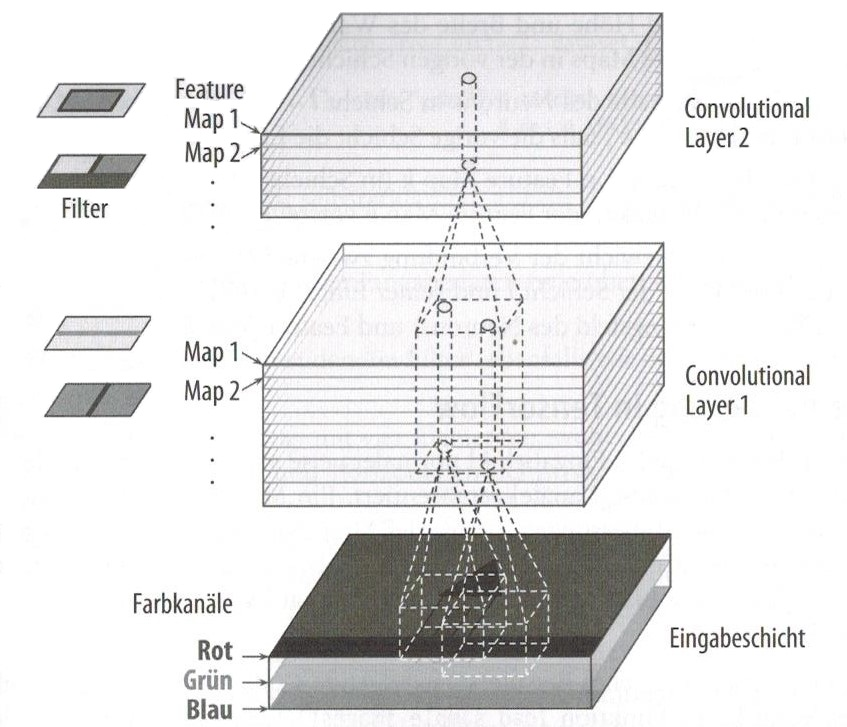
\includegraphics[width=11cm]{Bilder/feature_maps.jpeg} 
		\caption[Feature Maps]{Feature Maps \cite{AurelienGeron.2018}}
		\label{feature_maps}
	\end{center}
\end{figure}

Falls zusätzlich eine Farberkennung gewünscht ist, besitzt der Input Layer für jeden der drei Farbkanäle des RGB-Schemas eine Schicht, die Werte zwischen 0 und 255 in ihren LTUs tragen und den Stärken des Rot-, Grün- und Blaukanals entsprechen. \cite[S. 364 f.]{AurelienGeron.2018}

Der Lernprozess bei der Bilderkennung beruht nun darauf, die optimalsten Filter für die gegebene Aufgabe zu finden und diese zu komplexen Mustern zusammen setzen zu können. \cite[S. 363 f.]{AurelienGeron.2018}

Der zweite Grundbaustein eines CNN sind Pooling Layer. Ähnlich zu den Convolutional Layern ist auch hier jede LTU nur mit einer begrenzten Anzahl an LTUs des vorhergegangenen Layers verbunden, also nur mit dem lokalen Wahrnehmungsfeld. Der Hauptunterschied liegt aber darin, das keine Filter existieren, die die Eingaben unterschiedlich gewichten und dabei Muster erkennen, sondern stattdessen Aggregatfunktionen wie \textit{MAX()} oder \textit{MEAN()} dazu benutzt werden, um Eingaben zu verkleinern. So wird beispielsweise bei einem MAX-Pooling Layer mit Schrittweite größer als 1 der jeweils größte Wert des lokalen Wahrnehmungsfeld weitergereicht und durch die gewählte Schrittweite das vorherige Ergebnis verkleinert (siehe Abbildung \ref{pooling_layer}), was mit einem Informationsverlust verbunden ist. Dies ist allerdings ein wesentlicher Schritt, um weiter abstrahieren zu können. \cite[S. 369 f.]{AurelienGeron.2018}

\begin{figure}[ht]
	\begin{center}
		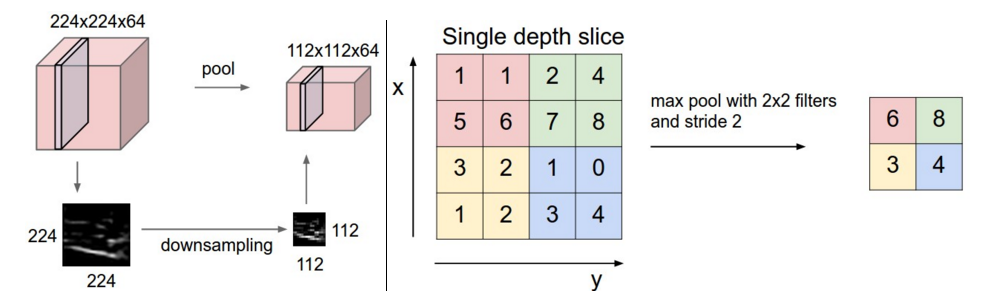
\includegraphics[width=15cm]{Bilder/pooling_layer.png} 
		\caption[Pooling Layer]{Pooling Layer \cite{LeonadroAraujoSantos.2018}}
		\label{pooling_layer}
	\end{center}
\end{figure}

Daneben ist ein Pooling über die Tiefe der Feature Maps möglich, hier bleibt die Größe der resultierenden Feature Maps gleich, die Anzahl verringert sich allerdings. \cite[S. 370]{AurelienGeron.2018}

Nachdem nun beide Grundbausteine eines CNNs genauer erläutert wurden, lassen sich diese nun kombinieren um ein vollständiges CNN zu bauen. Hierbei gibt es unterschiedlichste Architekturen, größtenteils äußerst komplexe. Im Rahmen dieser Arbeit genügt es allerdings die grundlegende Architektur zu erläutern.

Diese beginnt mit einigen Convolutional Layern, die aufeinander folgen und am Ende durch eine ReLU-Funktion nochmals gefiltert und durch ein Pooling Layer abgeschlossen werden. Dies wird je nach Komplexität der zu erkennenden Muster und der Größe der Bilder einige Male wiederholt. Das ursprüngliche Bild wird durch die Pooling Layer zwar immer kleiner, allerdings auch durch die Convolutional Layer immer tiefer. Das CNN schließt mit einem normalen Feed-Forward ANN mit vollständig verbundenen Schichten ab und trifft durch eine Softmax-Funktion eine Klassifikationsaussage des Bildes. \cite[S. 371]{AurelienGeron.2018}

Diese Architektur ermöglicht ebenso die Wiederverwendbarkeit einzelner Schichten und Gewichtungen für ähnliche Klassifikationsprobleme, bei denen gleiche Muster vorzufinden sind. \cite[S. 271]{AurelienGeron.2018}

\subsection*{Mean Average Precision}

Um die Genauigkeit von Objektdetektoren zu messen, wird oft die Metrik \textit{mean Average Precision} (mAP) gewählt. Diese setzt sich aus zwei grundlegenden Größen zusammen:

\begin{equation} \label{precisionandrecall}
\begin{split}
Precision = \frac{True Positive}{True Positive + False Positive} \\
\\
Recall = \frac{True Positive}{True Positive + False Negative}
\end{split}
\end{equation}
\equations{Precision und Recall}

\textit{Precision} sagt also etwas über die Verlässlichkeit einer Klassifikation aus, während \textit{Recall} Aussagen über die Erkennungsfähigkeit eines Objektdetektors trifft. Wichtig ist es hierbei anzumerken, dass mehrfach detektierte Objekte nur einmal als positiver Befund aufgefasst werden, die restlichen Detektionen gehen als \textit{False Positives} ein \cite{PaulHenderson.2017}.

\begin{figure}[ht]
	\begin{center}
		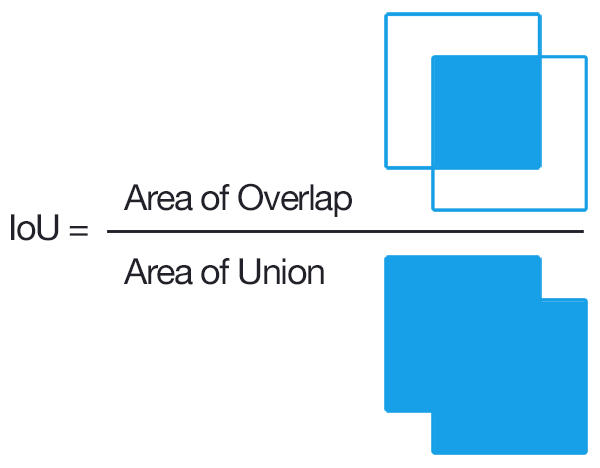
\includegraphics[width=8cm]{Bilder/iou_equation.png} 
		\caption[Intersection over Union]{Intersection over Union \cite{AdrianRosebrock.20161107}}
		\label{iou}
	\end{center}
\end{figure}

Die Tatsache, ob eine Bounding Box das gewünschte Objekt enthält und demnach ein positiver Fall vorliegt, wird anhand des \textit{confidence scores} bestimmt. Er berechnet sich aus der Multiplikation der Wahrscheinlichkeit für eine Klasse mit der sogenannten \textit{Intersection over Union} (IoU) (siehe Abbildung \ref{iou}) der jeweiligen ausgewählten Bounding Box. Die \textit{IoU} beschreibt ein Maß der Überdeckung der detektierten Bounding Box zur wahren Bounding Box. Der \textit{confidence score} sagt also etwas über die Gewissheit der Klassifikation aus. Für den kompletten Datensatz werden nun für unterschiedliche \textit{confidence scores} jeweils \textit{Precision} und \textit{Recall} bestimmt und anschließend in einem Graphen aufgetragen. Meistens werden die \textit{confidence scores} so gewählt, sodass sich eine äquidistante Abstufung in den \textit{Recall} Werten ergibt \cite{DingfuZhouJinFangXibinSongChenyeGuanJunboYinYuchaoDaiRuigangYang.2019}. 

\begin{figure}[ht]
	\subfigure{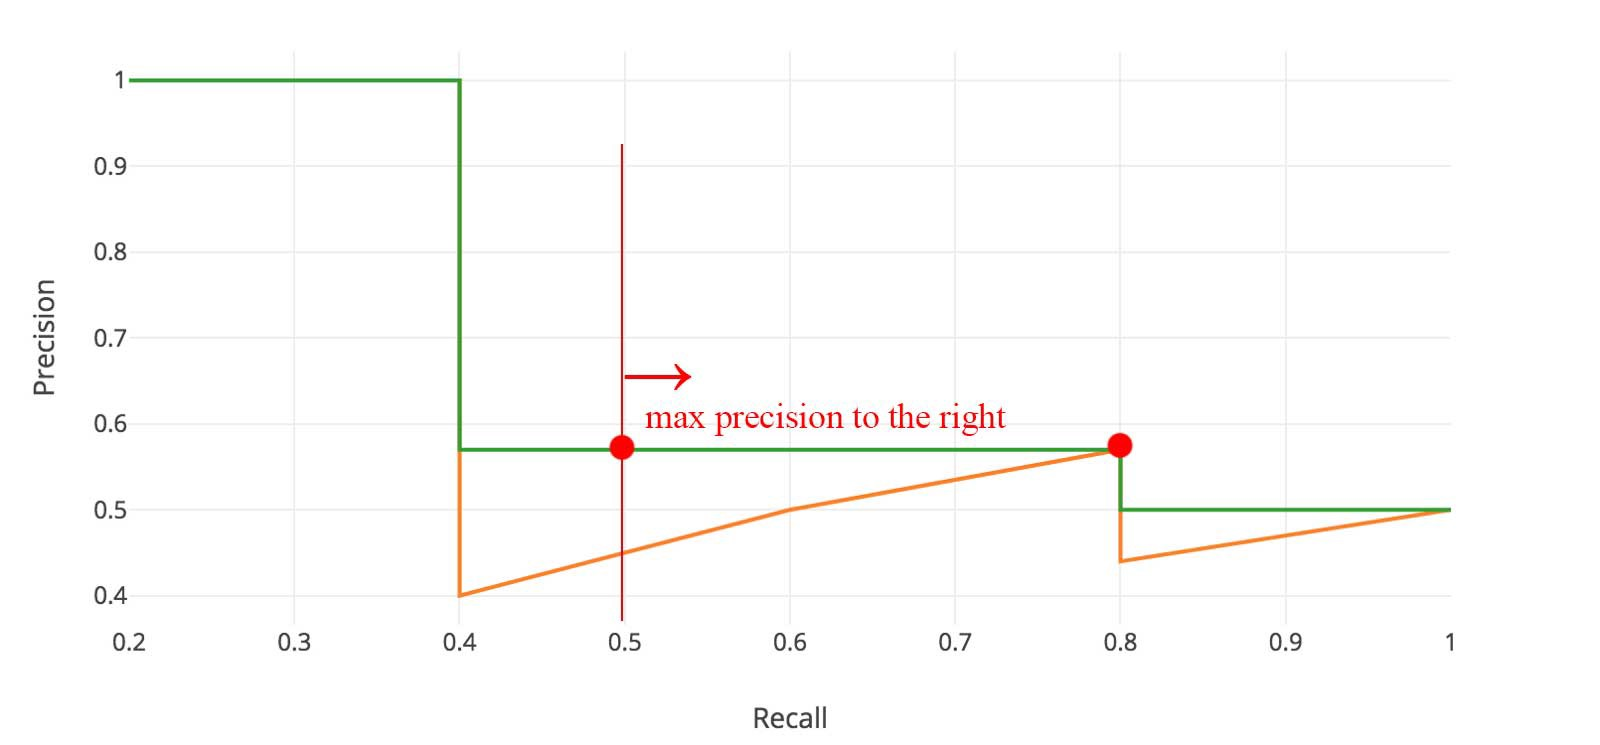
\includegraphics[width=12cm]{Bilder/map_graph1.png}} 
	\subfigure{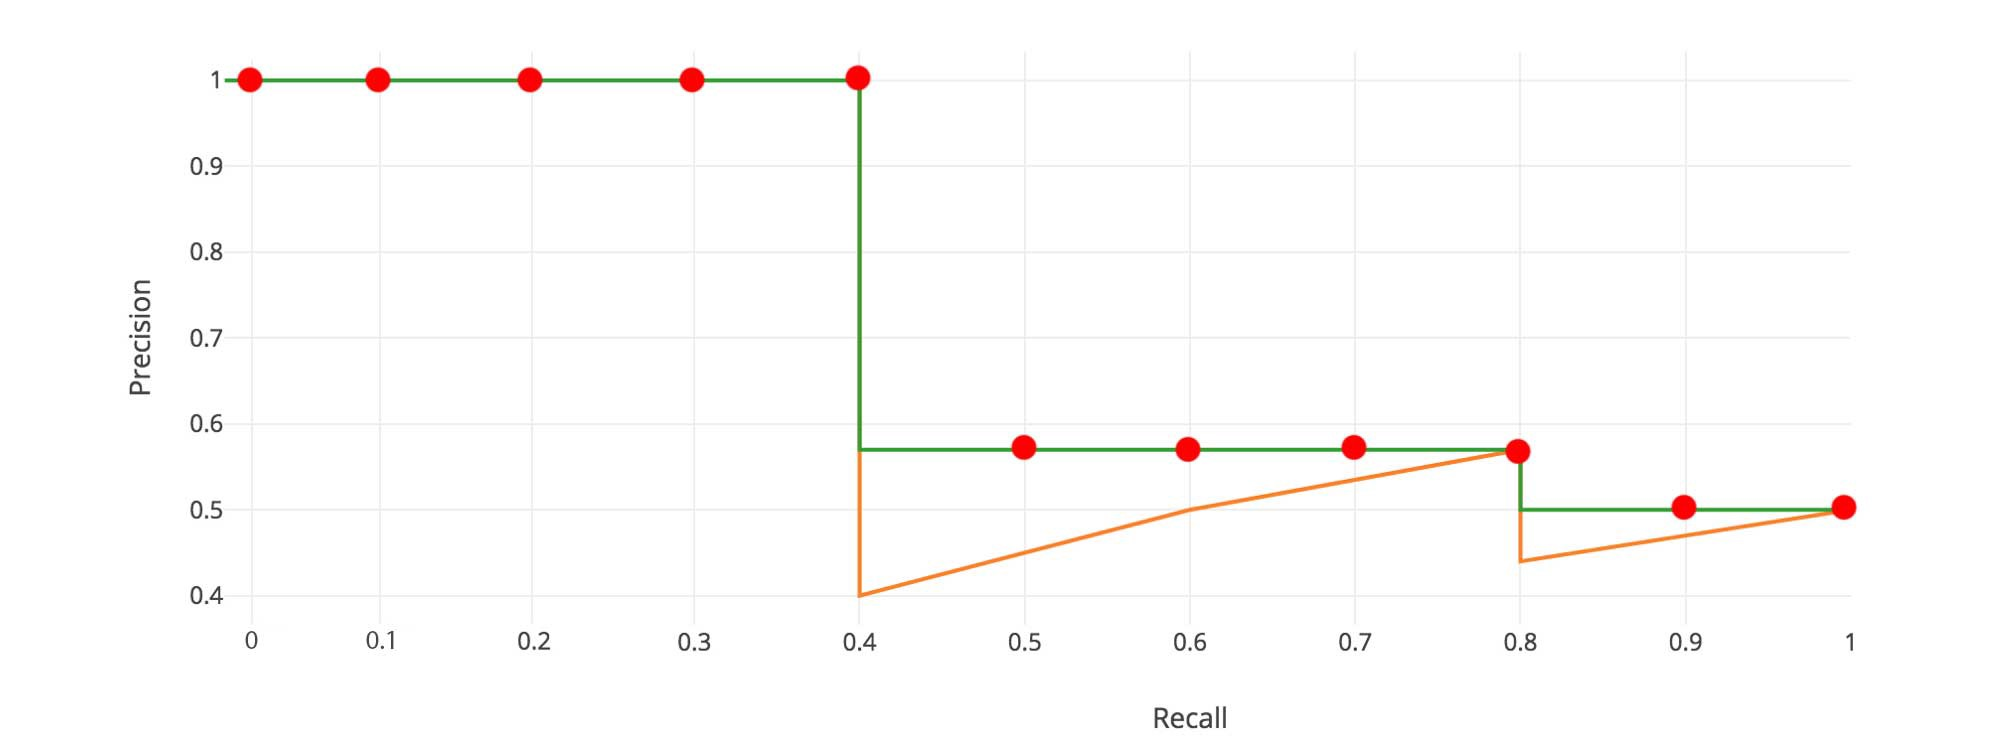
\includegraphics[width=12cm]{Bilder/map_graph2.png}} 
	\caption[Berechnung mAP]{Berechnung mAP \cite{JonathanHui.20180307}} 
	\label{map}
\end{figure} 

Im Graphen ist meist ein klassisches \glqq Zick-Zack\grqq{} Muster zu erkennen (siehe Abbildung \ref{map}). Dieses Muster wird geglättet, indem nach jedem Einbruch für jeden \textit{Recall} Wert der maximale \textit{Precision} Wert rechts des aktuellen \textit{Recalls} übernommen wird. Wird anschließend das diskrete Integral über alle \textit{Recall} Werte gebildet, so ergibt sich der \textit{Average Precision} Wert für eine zu klassifizierende Kategorie. Der Mittelwert der  \textit{Average Precisions} über alle Klassifikationskategorien hinweg ergibt letztendlich den \textit{mAP} Wert \cite{JonathanHui.20180307}. 

\section{Objektdetektoren} \label{detection}

Ein Teilziel der Machbarkeitsstudie ist es, anhand vorbestimmter Kriterien eine ausgewählte Menge von Objektdetektoren zu vergleichen. Um im Laufe der Arbeit zu verstehen, wie diese Auswahl zu Stande kommt und wie sich bestimmte Ergebnisse im Vergleich begründen lassen, ist eine Einführung in die unterschiedlichen Architekturen der Objektdetektoren unumgänglich. 

\subsection*{Regional Convolutional Neural Networks}

\textit{Regional Convolutional Neural Networks} (R-CNNs) vertreten den Ansatz, für ein Bild mehrere Lokationsvorschläge für mögliche Objekte zu liefern, sogenannte \textit{Regions of Interest} (RoIs), und diese anschließend zu klassifizieren. 

\begin{figure}[ht]
	\begin{center}
		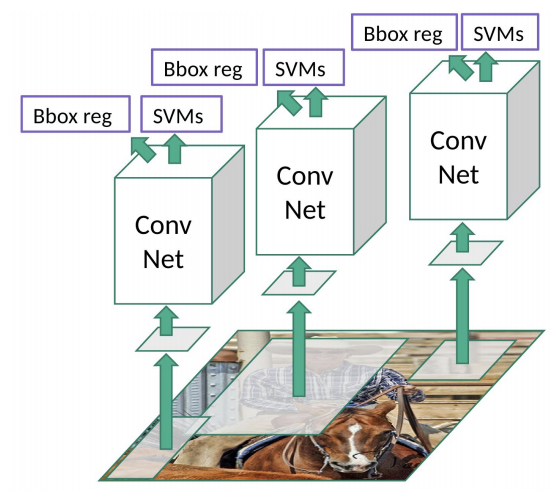
\includegraphics[width=8cm]{Bilder/rcnn.png} 
		\caption[R-CNN Architektur]{R-CNN Architektur \cite{RohithGandhi.20180709}}
		\label{rcnn}
	\end{center}
\end{figure}

Bei dem klassischen \textit{R-CNN} Detektor werden durch den \textit{Selective Search} Algorithmus 2000 solcher \textit{RoIs} vorgeschlagen. Zur Merkmalsextraktion wird für jede \textit{RoI} anschließend ein CNN eingesetzt. Der resultierende \textit{Feature Vektor} wird zur Klassifikation eines Objektes einer \textit{Support Vector Machine} (SVM) unterzogen. Um zusätzlich die Bounding Boxen akkurat zu bestimmen, wird der \textit{Feature Vektor} zudem einem \textit{Bounding Box Regressor} unterzogen (siehe Abbildung \ref{rcnn}) \cite{RossGirshickJeffDonahueTrevorDarrellJitendraMalik.2016}. 

Da der sogenannte \textit{Region Proposal} Schritt durch den \textit{Selective Search} Algorithmus allerdings viel Zeit in Anspruch nimmt, entstand eine Weiterentwicklung des \textit{R-CNN } Netzes, das \textit{Fast R-CNN} Netz. Dieses tauscht den Schritt des \textit{Selective Search} Algorithmus mit dem Einsatz des CNNs. Außerdem wird das klassische CNN leicht angepasst. Bei \textit{Fast R-CNN} wird ein Bild zunächst einem CNN unterworfen. Bevor eine \textit{Feature Map} durch \textit{Fully-Connected Layer} zu einem einzigen \textit{Feature Vektor} vereinfacht wird, werden aus der \textit{Feature Map} die verschiedenen \textit{RoIs} extrahiert. Dies geschieht wiederrum mit dem \textit{Selective Search} Algorithmus, mit dem Unterschied, dass dieser nun nur auf der \textit{Feature Map} operiert und nicht auf dem gesamten Bild. Durch \textit{RoI Pooling Layer} werden die einzelnen entstandenen Regionen in eine feste Größe transformiert und einzeln einer Klassifikation durch \textit{Fully-Connected Layer} und einer Softmax-Funktion unterworfen. Die Komponente mit dem \textit{Bounding Box Regressor} bleibt gleich. Durch den Tausch des CNNs mit dem \textit{Selective Search} Algorithmus werden die mathematischen Faltungsoperationen nur einmal statt 2000 Mal pro Bild ausgeführt, was die Performanz des Detektors gegenüber eines klassischen \textit{R-CNNs} enorm steigert \cite{RossGirshick.2015}.

\begin{figure}[ht]
	\begin{center}
		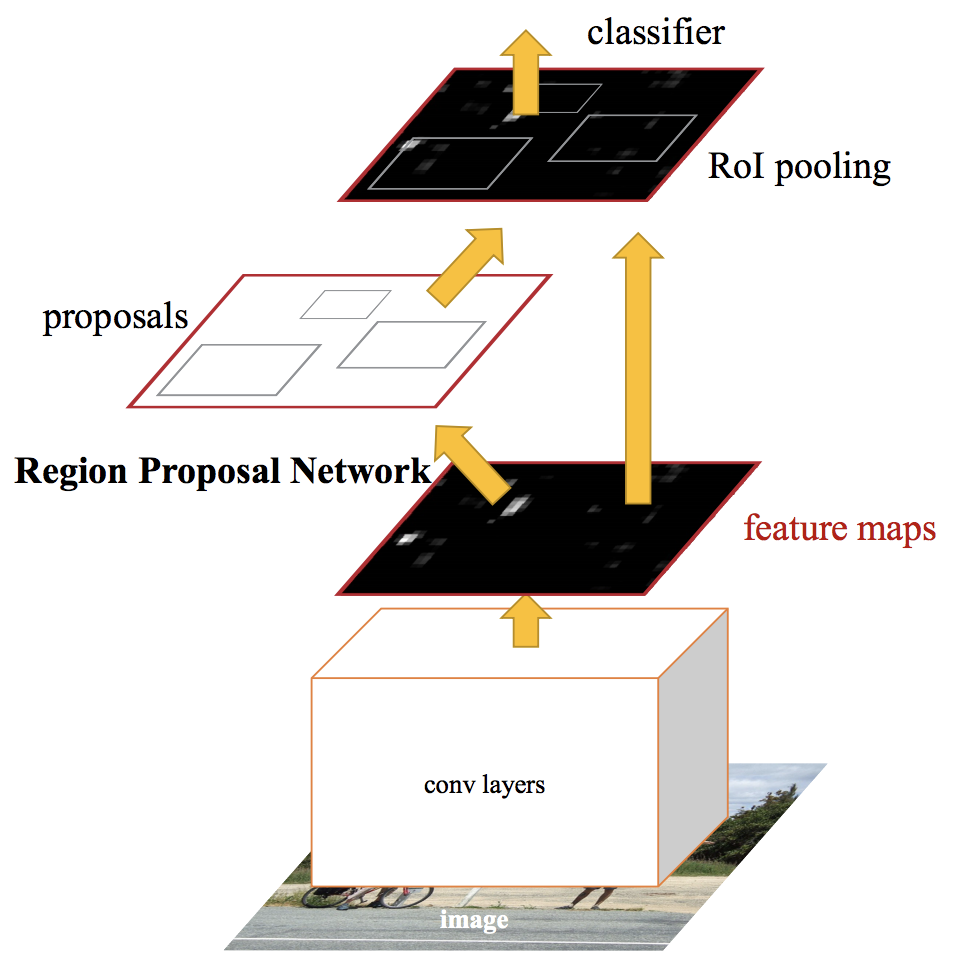
\includegraphics[width=8cm]{Bilder/fasterrcnn.png} 
		\caption[Faster R-CNN Architektur]{Faster R-CNN Architektur \cite{RohithGandhi.20180709}}
		\label{fasterrcnn}
	\end{center}
\end{figure}

Die letzte Optimierung der \textit{R-CNN} Familie entstand durch das \textit{Faster R-CNN} Netz. Dieses ersetzt den statischen \textit{Selective Search} Algorithmus des \textit{Fast R-CNN} Detektors durch ein eigenes lernfähiges, sogenanntes \textit{Region Proposal Network} (RPN)  (siehe Abbildung \ref{fasterrcnn}) \cite{ShaoqingRenKaimingHeRossGirshickJianSun.2016}.

Neben dem Einsatz von \textit{R-CNN} Detektoren zur Objektdetektion existiert ebenso ein Ansatz zur instanzbasierten Segmentierung, das \textit{Mask R-CNN} Netz. Es nimmt zwei wichtige Anpassungen an der Architektur des \textit{Faster R-CNN} Netzes vor. Da bei Segmentierungsproblemen eine genauere Abgrenzung von Objekt und Hintergrund notwendig ist, wird das \textit{RoI Pooling Layer} durch ein \textit{RoI Align Layer} ausgetauscht. Hierbei wird das Rundungsproblem beim Pooling behoben. Angenommen eine \textit{RoI} von 16x16 Pixeln wird mit einem \textit{MEAN-Pooling Layer} der Schrittweite Drei verarbeitet, so ergibt sich pro Pooling Schritt ein Einzugsgebiet von 5.33 Pixeln. Dieses wurde abgerundet auf 5 Pixel. Bei \textit{RoI Align Layern} wird durch bilineare Interpolation der Wert des 5.33ten Pixels ermittelt und in das Pooling mit einbezogen. Dies ermöglicht eine genauere Segmentierung an den Grenzen eines Objektes.

Außerdem wird parallel zum RPN ein sogenanntes \textit{Fully-Convolutional Network} (FCN) eingesetzt, einem Netz, dass rein aus \textit{Convolutional Layern} besteht. Es dient, um für jede existierende Klasse eine pixelbasierte binäre Maske auszugeben, die für jeden Pixel die Zugehörigkeit zu einer Klasse bestimmt. Basierend auf dieser Maske werden die detektierten Objekte anschließend farblich hervorgehoben \cite{KaimingHeGeorgiaGkioxariPiotrDollarRossGirshick.20180224}.
\subsection*{Single Shot MultiBox Detector}

Zwar liefern die oben genannten Objektdetektoren akkurate Ergebnisse, allerdings sind sie als zu rechenintensiv und langsam einzuordnen, als dass sie für Echtzeit Applikationen eingesetzt werden könnten. Der \textit{Single Shot MultiBox Detector} (SSD) unterschiedet sich von den vorhergegangenen Modellen dahingehend, dass er bewusst auf den Schritt der Generierung von Bounding Box Vorschlägen und des \textit{Poolings} verzichtet, um wesentlich schneller ablaufen zu können als andere Objektdetektoren. Die Präzision der Klassifikationen bleibt hierbei erhalten, selbst Bilder niedriger Auflösung können weiterhin verarbeitet werden. Dem \textit{SSD} genügt also ein einziges tiefes neuronales Netz zum Lokalisieren und Klassifizieren von Objekten. Wie der \textit{SSD} aufgebaut ist und welche Ansätze er verfolgt, soll in diesem Unterkapitel erläutert werden \cite{ssd.20161229}. 

\begin{figure}[ht]
	\begin{center}
		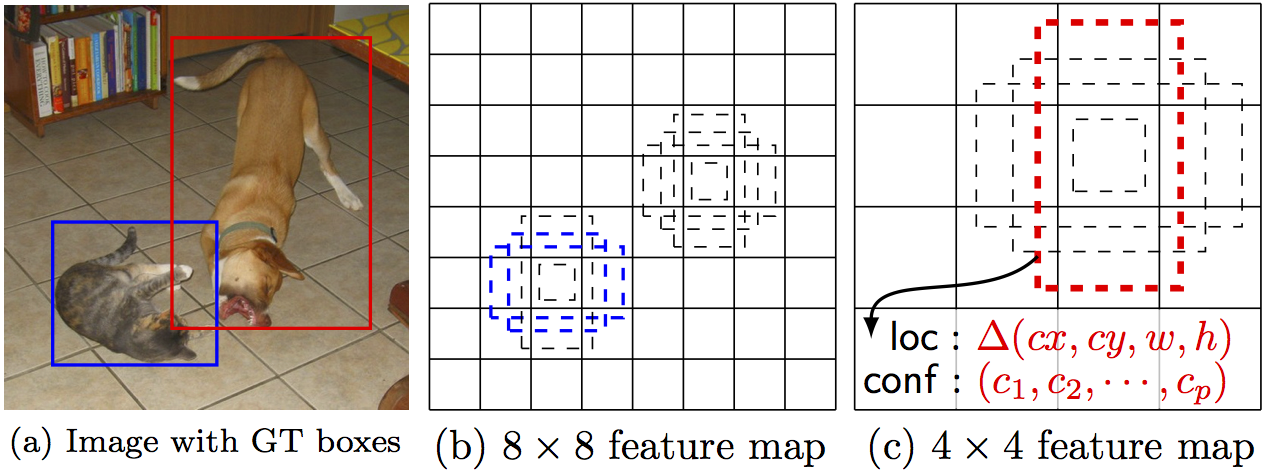
\includegraphics[width=15cm]{Bilder/ssd_framework.png} 
		\caption[SSD Grundprinzip]{SSD Grundprinzip \cite{ssd.20161229}}
		\label{framework}
	\end{center}
\end{figure}

Die Architektur des \textit{SSD} zielt zunächst darauf ab, ein Bild in mehrere unterschiedliche Gitterstrukturen zu unterteilen, die sich nach ihrer Skalierung unterscheiden. Dadurch ist es möglich Objekte unterschiedlicher Größe zu erkennen. Jede Lokation im Gitter besitzt eine gleiche Anzahl an festen, vordefinierten Bounding Boxen, die unterschiedliche Seitenverhältnisse aufweisen (siehe Abbildung \ref{framework}). So wird sichergestellt, dass sowohl horizontal als auch vertikal ausgeprägte Objekte in der selben Lokation gleichzeitig erkannt werden können (siehe Abbildung \ref{boundingboxes}) \cite{ssd.20161229}.

\begin{figure}[ht]
	\begin{center}
		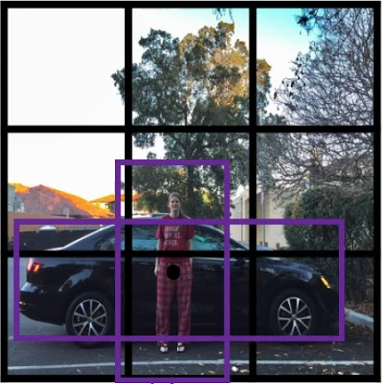
\includegraphics[width=7cm]{Bilder/bounding_boxes.png} 
		\caption[Bounding Boxes]{Bounding Boxes \cite{AndrewNg.2019}}
		\label{boundingboxes}
	\end{center}
\end{figure}

Für jede dieser Bounding Boxen bestimmt der \textit{SSD} Wahrscheinlichkeiten für Klassenzugehörigkeiten als auch Verschiebungen der vordefinierten Bounding Box zur wahren Bounding Box des Objekts für jede Klasse. Dies wird mit kleinen Faltungsfiltern erreicht, die in den hinteren Schichten des Netzwerks eingesetzt werden \cite{ssd.20161229}.

Die Kostenfunktion ist durch die gewichtete Summe des Lokalisationsverlustes und des Klassifikationsverlustes bestimmt. Während der Klassifikationverlust durch eine \textit{Softmax} Funktion bestimmt werden kann, wird der Lokalisationsverlust über die \textit{Smooth L1} Funktion (\ref{smooth}) bestimmt \cite{ssd.20161229}.

\begin{equation}\label{smooth}
\begin{split}
L_{loc}(t^u,v) = \sum\limits_{i \in (x,y,w,h)}^{n} SM_{L1}(t^u_i - v_i) \\
SM_{L1}(t^u_i - v_i) = \begin{cases}
							0.5x^2      & \text{wenn } |x| < 1\\
							|x| - 0.5   & \text{sonst}
						   \end{cases}
\end{split}
\end{equation}
\equations{Die Smooth L1 Funktion}

\begin{figure}[ht]
	\begin{center}
		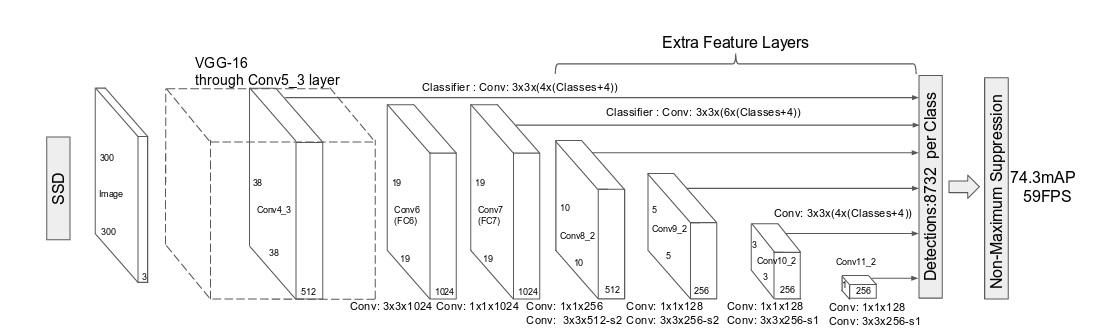
\includegraphics[width=15cm]{Bilder/ssd_architecture.png} 
		\caption[SSD Architektur]{SSD Architektur \cite{ssd.20161229}}
		\label{architecture}
	\end{center}
\end{figure}

Der \textit{SSD} benutzt ein \textit{VGG-16} Basis Netzwerk, um Klassifikationen zu ermöglichen. \textit{VGG-16} ist ein auf dem Datensatz von \textit{ImageNet} basierendes neuronales Netz, das bis zu 1000 unterschiedliche Kategorien klassifizieren kann \cite{MathWorks.2019b}. Unabhängig vom Basisnetzwerk werden Convolutional Layer als Hilfsstrukturen zur Objektdetektion eingesetzt. Diese verarbeiten die Bilder unterschiedlicher Gittergrößen, wobei die Gittergröße mit fortschreitenden Convolutional Layern abnimmt. Jeder Convolutional Layer kann eine feste Anzahl an Detektionen bestimmen. Eine Detektion wird durch eine Klassenangabe und die Lage einer vorhergesagten Bounding Box bestimmt. Eine Bounding Box wird durch einen Eckpunkt $P(x,y)$ und eine Höhe und Breite bestimmt. Bei $c$ Klassen hat der Ausgangsvektor demnach die Größe $c+4$. Für jede vordefinierte Bounding Box werden, falls vorhanden, die Koordinaten der originalen Bounding Box ermittelt dabei relativ zur vordefinierten Bounding Box abgespeichert. Die Zuordnung einer Bounding Box zu einer vordefinierten Bounding Box erfolgt über die sogenannte \textit{Intersection over Union} (IoU) (siehe Abbildung \ref{iou}). Überschreitet diese einen Wert von 0.5, so ist diese der originalen Bounding Box zugeordnet \cite{ssd.20161229}. Demnach ist es möglich, dass eine originale Bounding Box mehreren vordefinierten Bounding Boxen zugeordnet werden kann \cite{ssd.20161229} .

\begin{figure}[ht]
	\begin{center}
		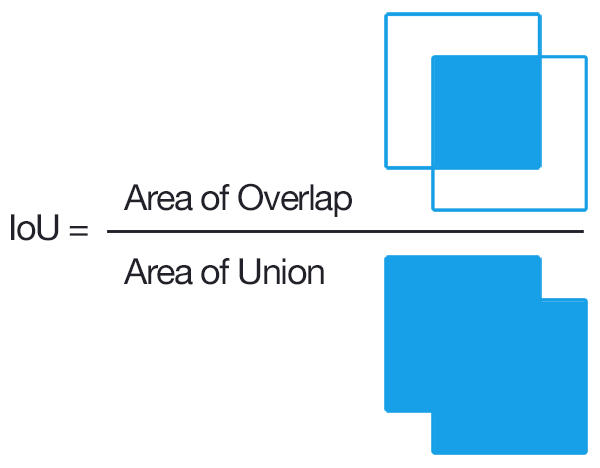
\includegraphics[width=8cm]{Bilder/iou_equation.png} 
		\caption[Intersection over Union]{Intersection over Union \cite{AdrianRosebrock.20161107}}
		\label{iou}
	\end{center}
\end{figure}

Bei $m \cdot n$ Lokationen und $k$ verschiedenen vordefinierten Bounding Boxen pro Lokation ergeben sich also $m \cdot n \cdot k \cdot (c+4)$ verschiedene Werte für eine Feature Map. Die Merkmalsextraktion zur Klassifikation wird durch Faltung mit $3x3$ Filtern erreicht \cite{ssd.20161229}.

Dieser Vorgang wird für alle Feature Maps für alle Convolutional Layer durchgeführt. Die daraus folgende Menge an Detektionen wird durch ein \textit{Non Maximum Suppression Layer} in ihrer Größe reduziert. Als Maß zur Filterung wird die sogenannte \textit{Intersection over Union} (IoU) der detektierten Box zur wahren Box verwendet \cite{ssd.20161229}.

Während der Trainingsprozesses des \textit{SSD300}\footnote{SSD300 verwendet Bilder der Auflösung 300x300 Pixel. Alternativ existiert ebenso SSD512 für Bilder der Auflösung 512x512 Pixel. Die Bilder können jedoch auch kleiner als die vorgegebene Auflösung gewählt werden.} mit PASCAL VOC2007 wurde eine Lernrate von $\eta = 10^{-3}$ für das Mini-Batch Verfahren mit Batchgröße 32 und Moment $\beta = 0.9$ verwendet. Die Gewichtungen wurden \textit{Xavier} initialisiert. Nach 40.000 Iterationen wurde die Lernrate für 10.000 Iterationen auf $\eta = 10^{-4}$ reduziert und schließlich auf $\eta = 10^{-5}$ \cite{ssd.20161229}. 

\begin{figure}[ht]
	\begin{center}
		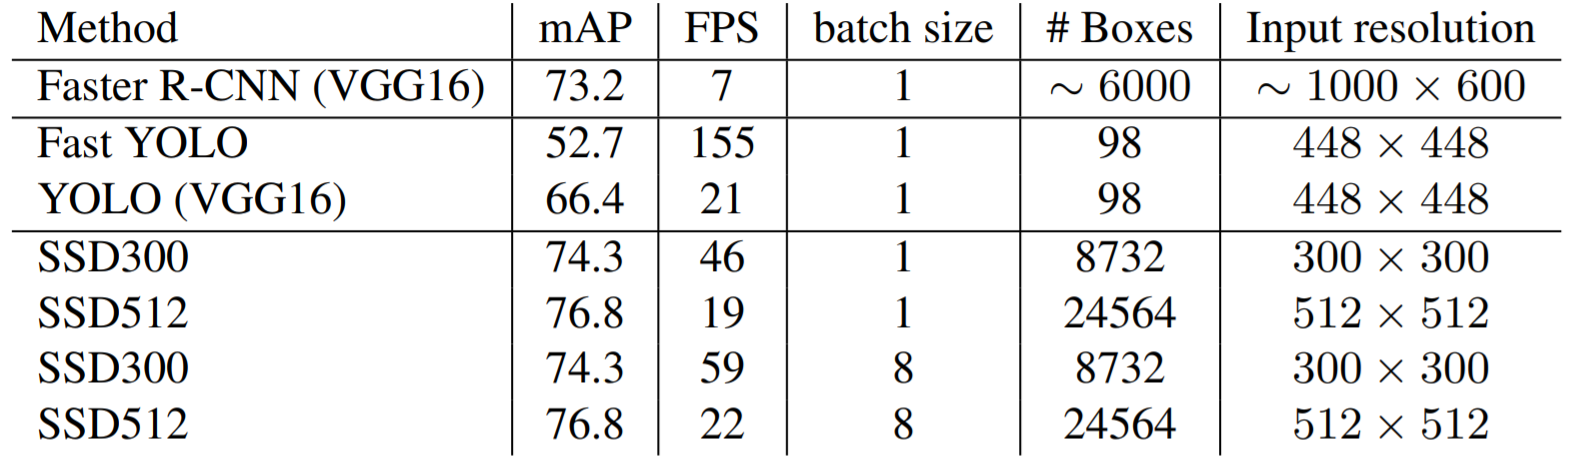
\includegraphics[width=12cm]{Bilder/ssd_results.png} 
		\caption[Vergleich SSD]{Vergleich SSD \cite{ssd.20161229}}
		\label{result}
	\end{center}
\end{figure}

Nach obiger Grafik ist eindeutig festzustellen, dass \textit{SSD300} ein gutes Verhältnis zwischen Präzision und Reaktionsvermögen bewahrt. Durch den Verzicht auf den Schritt der Generierung von Bounding Box Vorschlägen und des \textit{Poolings} kann \textit{SSD} deutlich schneller ablaufen als die Vergleichsdetektoren, während durch das Vordefinieren von Bounding Boxen ebenso eine hohe Präzision erzielt werden kann \cite{ssd.20161229}.

Allerdings ergibt sich vor allem für kleine Objekte ein erschwertes Detektionsvermögen, da diese in den höherliegenden Convolutional Layern untergehen. Als Lösung hierfür kann eine erhöhte Inputgröße gewählt werden (vgl. \textit{SSD512}) oder Daten-Augmentierung für den Lernprozess angewandt werden. Weitere mögliche Fehler können falsche Positivbefunde aufgrund von fehlerhafter Lokalisation sein, Verwechslung mit ähnlichen Kategorien oder dem Hintergrund sowie weitere \cite{ssd.20161229}.

Letztendlich lässt sich \textit{SSD} als schneller Objektdetektor beurteilen, der nicht nur einfach zu trainieren und integrieren ist, sondern ebenso ein gutes Verhältnis zwischen Lokalisationspräzision und Echtzeitvermögen schafft.

\subsection{You Only Look Once}

Der Algorithmus \textit{You Only Look Once} (YOLO) ist ein weiterer Objekterkennungsalgorithmus und betrachtet statt separaten Bildregionen das komplette Bild. Er benutzt nur ein neuronales Netz, um Bounding Boxen und Wahrscheinlichkeiten für bestimmte Klassen vorherzusagen.

Hierzu wird ein $S \times S$ Gitter über das Bild gelegt. Für jedes Feld im Gitter werden $B$ Bounding Boxen erzeugt. Jede Box besitzt neben den zum Gitterfeld relativen Positionswerten einen Wert, der die Vorhersage der jeweiligen Klasse und die Präzision der Box repräsentiert. Dieser Wert wird als \textit{confidence score} bezeichnet und wird durch die Multiplikation der Wahrscheinlichkeit für eine Klasse mit der \textit{IoU}, also die Präzision der berechneten Box im Verhältnis zu der Box aus den vortrainierten Testdaten festgelegt \cite{JosephRedmon.2016}.

Aus der Menge an Bounding Boxen werden schließlich mit Hilfe eines festgelegten Schwellwertes die Boxen mit lokalisierten Objekten bestimmt (siehe Abbildung \ref{yolo_model}).

\begin{figure}[ht]
	\begin{center}
		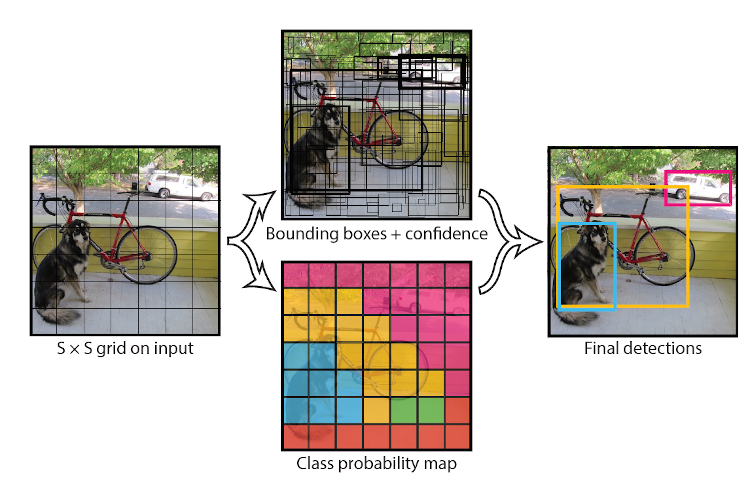
\includegraphics[width=15cm]{Bilder/yolo_model.png} 
		\caption{Vereinfachte Darstellung der Objekterkennung mit dem YOLO Algorithmus \cite{JosephRedmon.2016}}
		\label{yolo_model}
	\end{center}
\end{figure}

Die vorhergesagten Werte werden in einem $S \times S \times (B * 5 + C)$ Tensor kodiert, wobei $S$ und $B$ wie zuvor beschrieben durch das Gitter und die Bounding Boxen festgelegt sind und $C$ die Anzahl der Klassen definiert. Abbildung \ref{yolo_architecture} zeigt den Aufbau des CNN von \textit{YOLO} für die Detektion. Es besteht aus 24 Convolutional Layern gefolgt von 2 Fully-connected Layern. Für die Genauigkeit bei der Detektion wird die Auflösung des Bildes verdoppelt \cite{JosephRedmon.2016}. 

//TODO erkläre layer

In dem Netzwerk in Abbildung \ref{yolo_architecture} wird ein Bild mit einer Auflösung von $224 \times 224$ Pixeln verwendet und die vorhergesagten Werte im $7 \times 7 \times 30$ Tensor ausgegeben.

\begin{figure}[ht]
	\begin{center}
		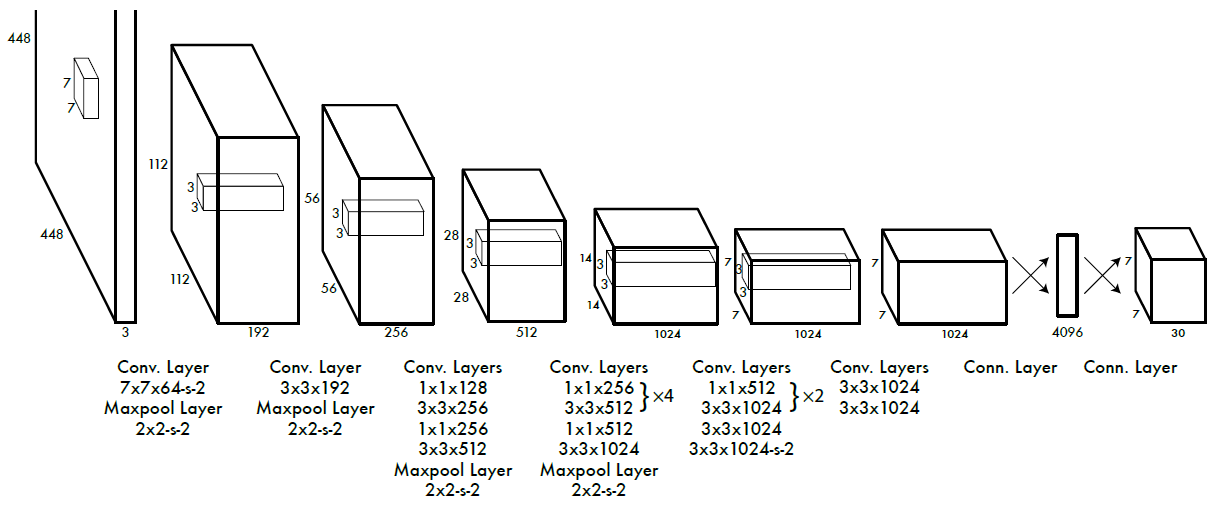
\includegraphics[width=15cm]{Bilder/yolo_architecture.png} 
		\caption{\textit{YOLO} Architektur \cite{JosephRedmon.2016}}
		\label{yolo_architecture}
	\end{center}
\end{figure}

Die mittlerweile dritte und aktuelle Version von \textit{YOLO} weist enorme Verbesserungen auf, gerade im Bezug auf die Erkennung von sehr kleinen Objekten wie zum Beispiel einzelne Vögel in einem Schwarm \cite{JosephRedmon.2018}.

TODO Veränderung im Netz: https://www.cyberailab.com/home/a-closer-look-at-yolov3







\section{Cloud Infrastruktur} \label{cloud}

Das Trainieren eines \textit{Deep Learning} Modells ist gerade bei großen CNN Architekturen rechenaufwendig. Tensor Operationen wie Matrixmultiplikationen und Konvolutionen erfordern im Rahmen des maschinellen Lernens hohe Parallelisierung und Taktfrequenzen, um in absehbarer Zeit gute Ergebnisse zu liefern. Die Rechenkapazität normaler Desktop-PCs reicht meist nicht aus, um performantes \textit{Deep Learning} betreiben zu können. 

Abhilfe bieten Software-as-a-Service (SaaS) bzw. Platform-as-a-Service (PaaS) Angebote wie \textit{Amazon SageMaker}, \textit{Google Cloud Platform Cloud AI} oder \textit{Azure ML Services} oder aber auch Start-ups wie \textit{FloydHub}. Diese bieten Infrastruktur in unterschiedlichen Zonen je nach Standpunkt der Rechenzentren zum Trainieren an sowie eine Plattform zum Verwalten der \textit{Deep Learning} Prozesse. 

\subsection*{Trainingshardware}

Gerade GPUs bieten sich aufgrund ihres hohen Parallelisierungsvermögens gegenüber herkömmlichen CPUs an. Insbesondere \textit{NVIDIA} nimmt hierbei eine Vorreiterrolle in der Produktion von Server-GPUs ein. Die \textit{Compute Unified Device Architecture} (CUDA) von \textit{NVIDIA} ermöglicht als Programmiermodel und parallele Computing Plattform das Auslagern von Rechenprozessen auf GPUs. Das \textit{CUDA} Toolkit beinhaltet GPU beschleunigte Bibliotheken, einen Compiler, Entwicklungswerkzeuge sowie die eigentliche \textit{CUDA} Laufzeit und wird von vielen \textit{Deep Learning} Bibliotheken genutzt, wie z.B. \textit{PyTorch} \cite{NVIDIA.20200209, PyTorch.20200209}. Hauptvergleichskriterien zwischen GPUs sind hierbei der Grad der möglichen Parallelisierung und die reine Rechenleistung im Verhältnis zum Stromverbrauch.

Neben GPUs existieren seit 2015 die von Google entwickelten \textit{Tensor Processing Units} (TPUs). Diese sind speziell entwickelte, anwendungsspezifische integrierte Schaltung (engl.: \textit{Application-Specific Integrated Circuit}) (ASIC) für Arbeitslasten im maschinellen Lernen \cite{GoogleCloud.20200209b}.

Eine weitere Steigerung versprechen Microsofts Field Programmable Gate Arrays (FPGAs), die allerdings nicht weiter im Rahmen dieser Arbeit betrachtet werden sollen \cite{KarlFreund.20170828}.

\subsection*{Amazon Web Services SageMaker}

\textit{Amazon Web Services} (AWS) bietet mit \textit{SageMaker} eine integrierte Plattform zum Trainieren und Bereitstellen von \textit{Deep Learning} Modellen. Zentrales Alleinstellungsmerkmal ist das einheitliche Toolset, in dem alle Arbeitsprozesse rund um ein \textit{Deep Learning} Modell integriert abgebildet werden können. Es ist somit nicht mehr nötig, unterschiedliche Tools und Arbeitsabläufe zusammenfügen, was zuvor zeitaufwändig und fehleranfällig war \cite{AmazonWebServices.20200314}.

Außerdem bietet \textit{AWS SageMaker} die ersten vollständig integrierte Entwicklungsumgebung für Machine Learning, \glqq Amazon SageMaker Studio\grqq{}. Zum Erstellen der \textit{Deep Learning} Modellen werden sogenannte \textit{Amazon Sagemaker Notebooks} genutzt, eine Ableitung klassischer \textit{Jupyter Notebooks}. Unterstützte Frameworks sind TensorFlow, PyTorch, Apache MXNet, Chainer, Keras, Gluon, Horovod, Scikit-Learn und Deep Graph Library \cite{AmazonWebServices.20200314}. 

\textit{AWS SageMaker} bietet verschiedene Instanztypen an, die sich je nach Anzahl an vCPUs und GPUs unterscheiden. Auch der vorhandene Arbeitsspeicher, Grafikkartenspeicher und die Netzwerkleistung kann durch die Vielzahl an angebotenen Instanzen nach individuellen Bedürfnissen gewählt werden \cite{AmazonWebServices.20200314b}.

\subsection*{Google Cloud Platform AI Platform}

\textit{AI Platform} ist das Konkurrenzprodukt zu \textit{AWS SageMaker} von der \textit{Google Cloud Platform} (GCP). Die Plattform bietet ebenso verschiedene Komponenten für das \textit{Deep Learning} an. Hierzu gehören \textit{AI Platform Notebooks}, ein Dienst mit einer integrierten JupyterLab-Umgebung, \textit{Deep Learning} Virtual Machines (VM) mit vorinstalierten \textit{Deep Learning} Frameworks, verteiltes Training mit automatischer Hyperparameter-Abstimmung durch den \textit{AI Platform Training} Dienst oder \textit{AI Platform Prediction} zum Bereitstellen trainierter Modelle \cite{GoogleCloudPlatform.20200314}. 

Hervorzuheben sind insbesondere Googles \textit{Tensor Processing Units} (TPUs). Dies sind spezielle Hardwarebeschleuniger, die speziell für \textit{Deep Learning} Projekte im \textit{TensorFlow} Framework optimiert wurden und für jede Instanz in der GCP mobilisiert werden können. Dabei wird pro TPU-Kern eine Rechenleistung von bis zu 92 TOPS erreicht \cite{HaraldBogeholz.20170406}. Werden 2048 solcher TPU-Kerne zu einem TPU-Pod zusammen geschlossen, so ergibt sich eine Rechenleistung von über 100 PetaFLOPS \cite{GoogleCloud.20200209}. Zudem ist die größere Rechenleistung gleichzeitig effizienter als herkömmliche GPUs \cite{GoogleCloud.20200209b}. TPUs sind also darauf ausgelegt, ein optimales Preis-/Leistungsverhältnis beim Trainieren von \textit{Deep Leaning} Modellen zu erreichen \cite{GoogleCloudPlatform.20200314}.

\subsection*{Google Colab}

\textit{Google Colaboratory}, kurz \textit{Google Colab}, ist eine kostenfreie, cloudbasierte \textit{Jupyter Notebook} Umgebung von Google. Dokumente, die in Google Colab erstellt werden, werden automatisch mit \textit{Google Drive} synchronisiert. Die Laufzeit ist frei konfigurierbar zwischen Python 2 und 3 bzw. zwischen einfachem CPU, GPU oder TPU Computing. Nachteil an dem kostenfreien \textit{Google Colab} ist, dass zugewiesene Hardwareresourcen mit weiteren Nutzern geteilt werden müssen und so nicht die volle Rechenleistung für den individuellen Entwickler zur Verfügung stehen \cite{GoogleColaboratory.20200314}. 

Auch können keine längerfristigen Trainingsjobs ausgeführt werden, ohne dass nach 90 Minuten der Client von dem zugewiesenen Server getrennt wird \cite{GoogleCloud.20200314}.

\subsection*{Microsoft Azure}

\textit{Microsoft Azures} Angebot für \textit{Deep Learning} in der Cloud ist zunächst wenig transparent. Sie bieten ebenso wie Amazon und Google das Trainieren und Bereitstellen von \textit{Deep Learning} Modellen an und zudem eine einige DevOps Landschaft für solche Arbeitsprozesse. Auch werden Frameworks wie \textit{TensorFlow} oder \textit{PyTorch} unterstützt sowie das Programmieren in \textit{Jupyter Noteboks} \cite{MicrosoftAzure.20200314}.

\subsection*{FloydHub}

FloydHub, ein kalifornisches Start-up, bietet eine Data-Science Plattform zum Trainieren und Bereitstellen von \textit{Deep Learning} Applikationen. FloydHub erlaubt es Anwendern, sich auf reines \textit{Deep Learning} zu konzentrieren, während es die Arbeit rund um den \textit{Deep Learning} Lebenszyklus abnimmt. Hierzu gehört das Bereitstellen der entsprechenden Hardware, das Installieren von Treibern oder das Integrieren verschiedener \textit{Deep Learning} Bibliotheken, wie \textit{TensorFlow}, \textit{PyTorch} oder \textit{Keras} \cite{FloydHub.20200215}. 

Mit Hilfe des von FloydHub bereitgestellten Command Line Interfaces (CLI) kann ein lokales Projekt zu einem FloyHub Projekt initialisiert werden. Anschließend können anhand einer Konfigurationsdatei Einstellungen über das Training spezifiziert werden (siehe Listing \ref{floydhub:FloydHub}). Alternativ können diese auch über das CLI festgelegt werden. 

\lstset{language=XML}
\lstinputlisting[
label=floydhub:FloydHub,
caption=Konfigurationsdatei zum Trainingsjob auf FloydHub,
captionpos=b,
firstline=1,
lastline=9
]{Quellcode/floyd.yml}

Hierbei kann zwischen der K80 (gpu) oder der V100 (gpu2) GPU für das Training gewählt werden. Auch die \textit{Deep Learning} Laufzeitumgebung muss spezifiziert werden. Bei Bedarf auch zusätzliche Bibliotheken in einer \textit{floyd\_requirements.txt}-Datei zur Installation mit angegeben werden. Anschließend muss der Datensatz referenziert werden, mit dem das Modell trainiert werden soll. 

Dieser Datensatz wird separat hochgeladen, da sich dieser im Gegensatz zum Programmcode nur selten ändert. FloydHub implementiert auf seiner Plattform eine Art Pfadsystem, unter dem Datensätze und Projekte abgespeichert werden. Diese Pfade werden in der Konfigurations-Datei zur Referenzierung genutzt. Um auch im Programmcode auf den Datensatz zuzugreifen, muss ein Mountname definiert werden. In obigen Beispiel wird dem Datensatz unter Verzeichnis \textit{<username>/datasets/smartwarehousessd/3} der Mountname \textit{ssd} gegeben. Das Verzeichnis zum Einlesen der Daten ist anschließend im Code unter \textit{/floyd/input/ssd/} erreichbar. 

Mit dem CLI Befehl \textit{floyd run} wird der Programm Code auf die Plattform hochgeladen und der in der Konfigurationsdatei angegebene Befehl ausgeführt. Daraufhin wird ein Job erstellt, versioniert und ausgeführt. Während der Job ausgeführt wird, wird dem Nutzer ein Einblick in die Konsolenausgabe gewährt sowie in Metriken zur Hardwareauslastung. In der Jobhistorie kann im Nachhinein jeder Job mit dem damals aktuellen Programmcode und Datensatz eingesehen werden. Auch Datensätze werden versioniert. Schreibrechte sind auf das Verzeichnis \textit{/floyd/home} begrenzt, hier können Zwischenspeicherpunkte des Modells abgelegt werden. 

Neben klassischen Trainingsjobs können \textit{Deep Learning} Modelle auch ganz einfach in \textit{Jupyter Notebooks} erstellt werden. Hierzu muss in einem Projekt ein Workspace angelegt werden.



\section{Einführen von Bewertungskriterien}

Um Objektdetektoren miteinander vergleichbar zu machen und um deren Potential zum industriellen Einsatz zu bewerten, müssen konkrete Bewertungskriterien eingeführt werden.

\subsection*{Präzision}

Zur Messung der Präzision wird die Metrik \textit{mAP} verwendet. Dies garantiert eine gute Vergleichbarkeit mit den veröffentlichten Leistungsmerkmalen der Objektdetektoren.

\subsection*{Reaktionsvermögen}

Um eine Verarbeitung in Echtzeit zu ermöglichen, muss gewährleistet sein, dass die Inferenzgeschwindigkeit mit dem Modell mit der eingehenden Bildrate einhergeht. Als Maßstab dafür dient die \textit{Frames Per Second} (FPS) Zahl. Echtzeitfähigkeit in der Machbarkeitsstudie ist so definiert, dass die Inferenz mit dem Modell mindestens so schnell ablaufen muss, dass Änderungen in der Umgebung rechtzeitig von Objektdetektor noch wahrgenommen werden können. 

\subsection*{Trainingsverhalten}

Unter dem Punkt Trainingsverhalten wird zusammengefasst, wie schnell sich die einzelnen Modelle mit den unterschiedlichen Objektdetektoren trainieren lassen. Hierbei wird besonderer Fokus darauf gelegt, wie viele Trainingsepochen notwendig sind, bis der Gradient der Fehlerfunktion des neuronalen Netzes keine merkenswerten Fortschritte auf Basis des verwendeten Datensatzes mehr erzielt.

\subsection*{Inferenzverhalten}

Im Zuge der Evaluation des Inferenzverhaltens werden vier Kriterien betrachtet. 

\begin{itemize}
	\item Das Verhalten bei besonderen Beleuchtungsverhältnissen wie unterbeleuchteten oder überbeleuchteten Gegenden.
	\item Das Verhalten bei extremen Blicklagen auf Basis der Entfernung und des Winkels zum detektierenden Objekt.
	\item Das Verhalten bei nicht vollständig sichtbaren Objekten, z.B. bei Verdeckung.
	\item Der Umgang mit doppelt detektierten Objekten. 
\end{itemize}

\section{Initialer Vergleich der Objektdetektoren}

\begin{itemize}
	\item Synthetischer Datensatz
	\item Effekte/Probleme nachweisen
	\item Bewertungskriterien bestärken
	\item Hyperparameter bestimmen bzw. allgemein Problemlösungsverfahren
	\item Variantendiskussion (Welches Verfahren eignet sich hinsichtlich Bewertungskriterien am besten)
	\item Keine Bewertung der Detektoren!
\end{itemize}

Mögliche Probleme:
\begin{itemize}
	\item Mehrfach-Detektionen werden alle als positiv angesehen
\end{itemize} 

\section{Echtzeitumgebung}

Das \textit{SmartWarehouse} lehnt sich an ein großes Warenhaus an, bei dem Produkte nicht in Kartons verpackt sondern als ganzes auf Regalen angeordnet sind, ähnlich wie bei \textit{Baumarkt} oder \textit{Selgros}. Im Rahmen des Projektes wurde sich exemplarisch auf Flaschen konzentriert, dabei wurden neun Kategorien bestimmt (siehe Abbildung \ref{categories}). 

\begin{figure}[htb]
	\subfigure[Saskia Wasser Klein]{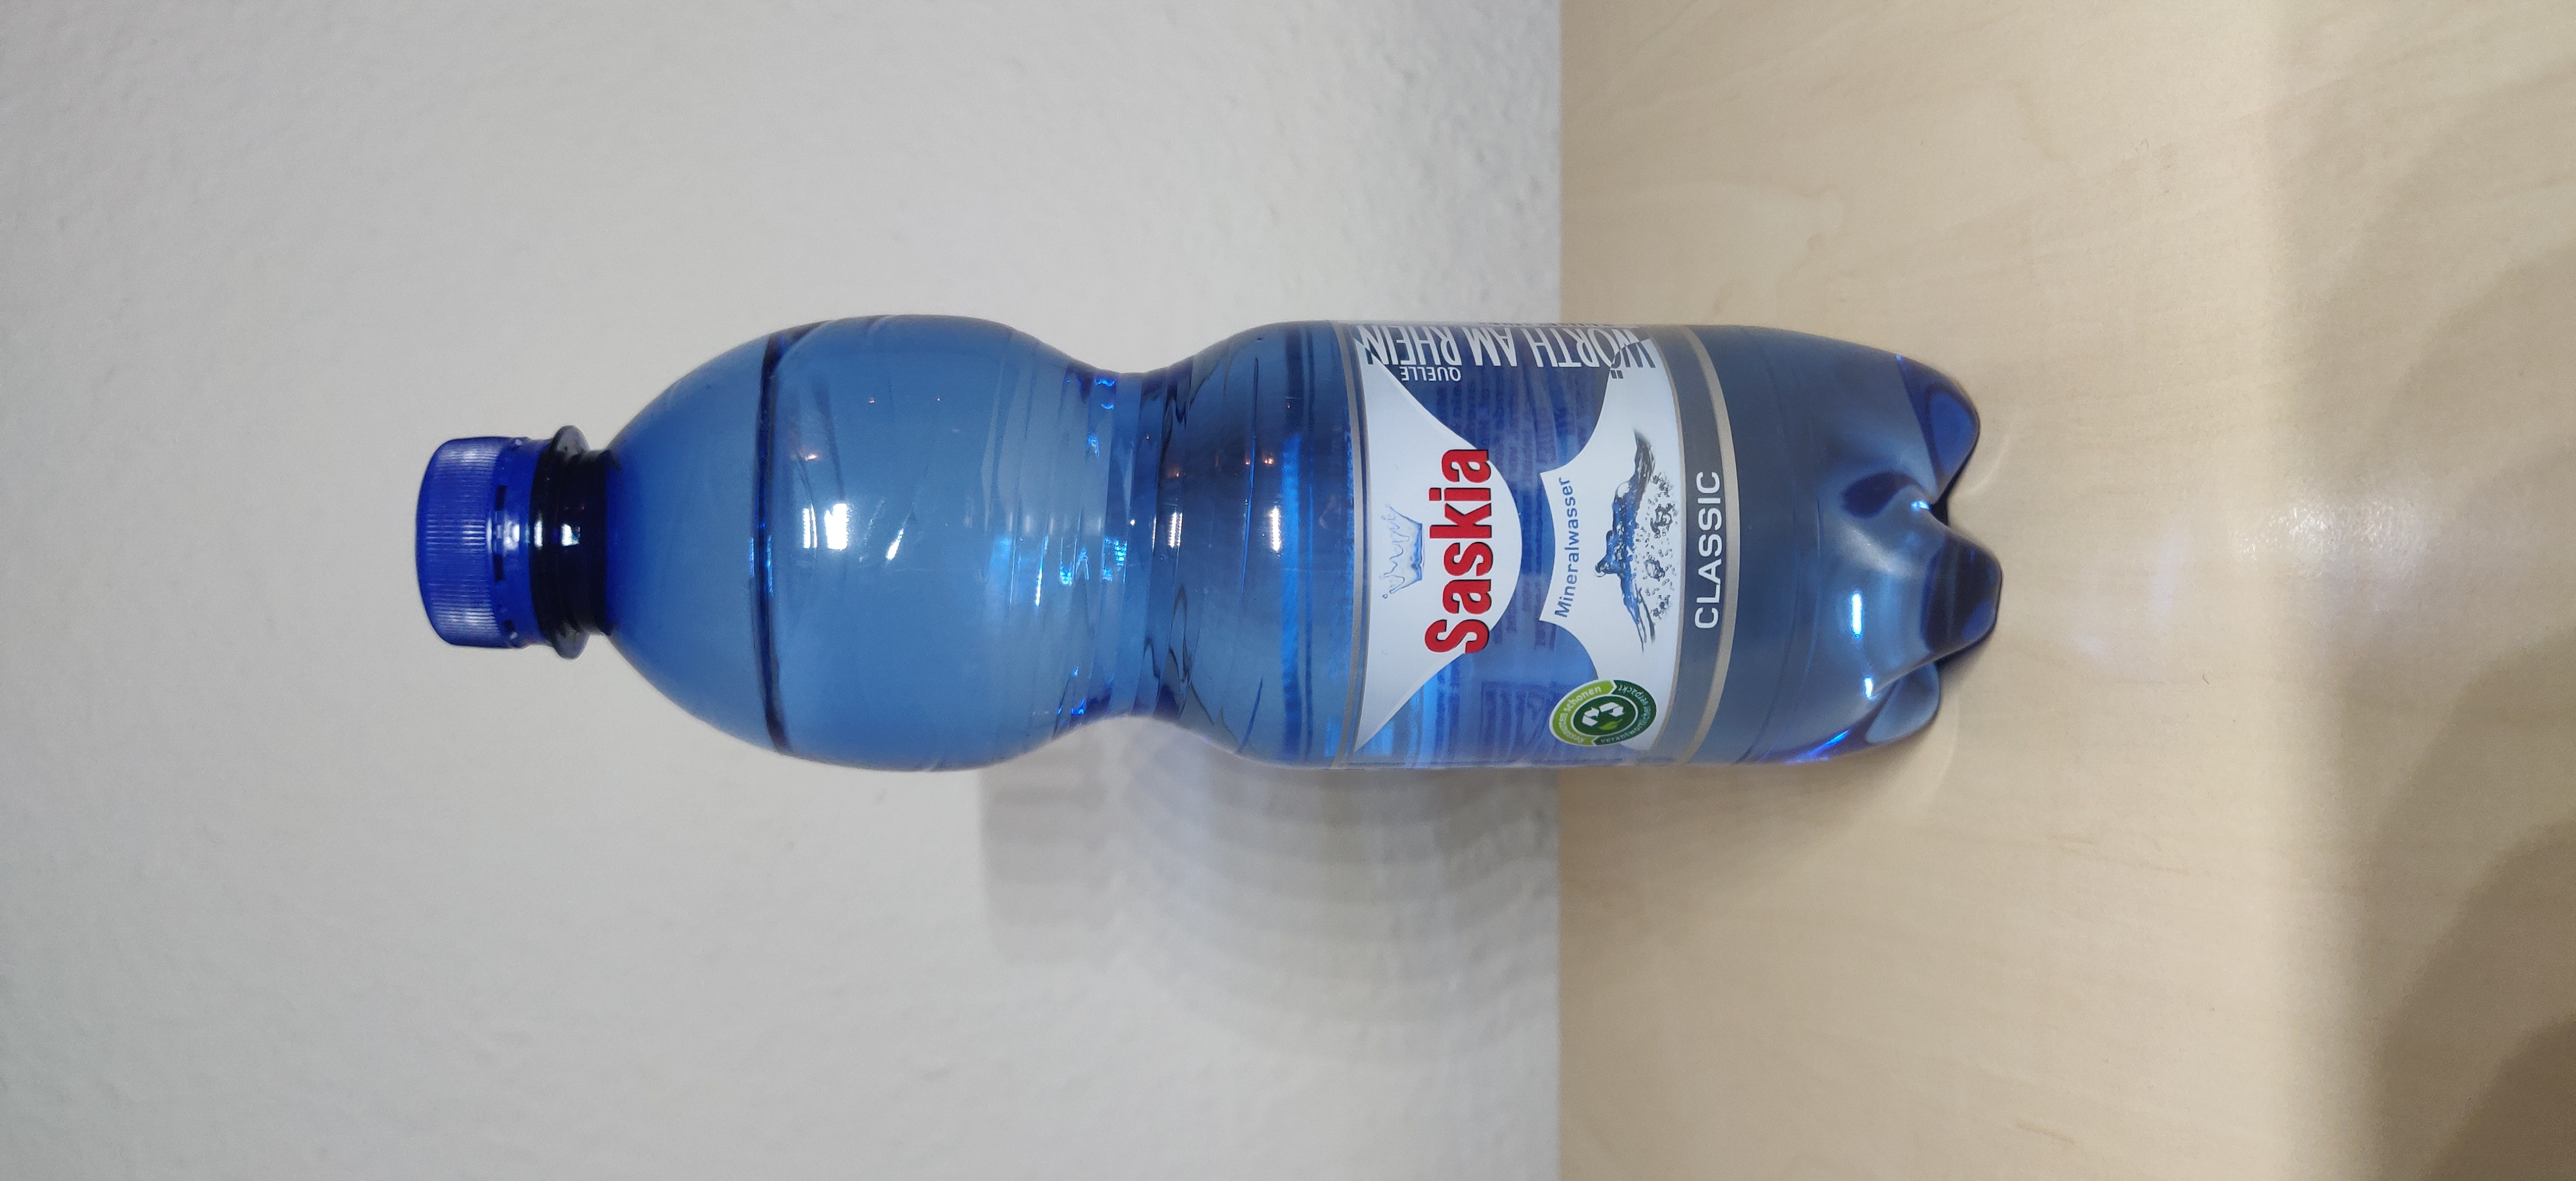
\includegraphics[width=0.32\textwidth]{Bilder/wasser_klein.jpg}}
	\subfigure[Saskia Wasser Groß]{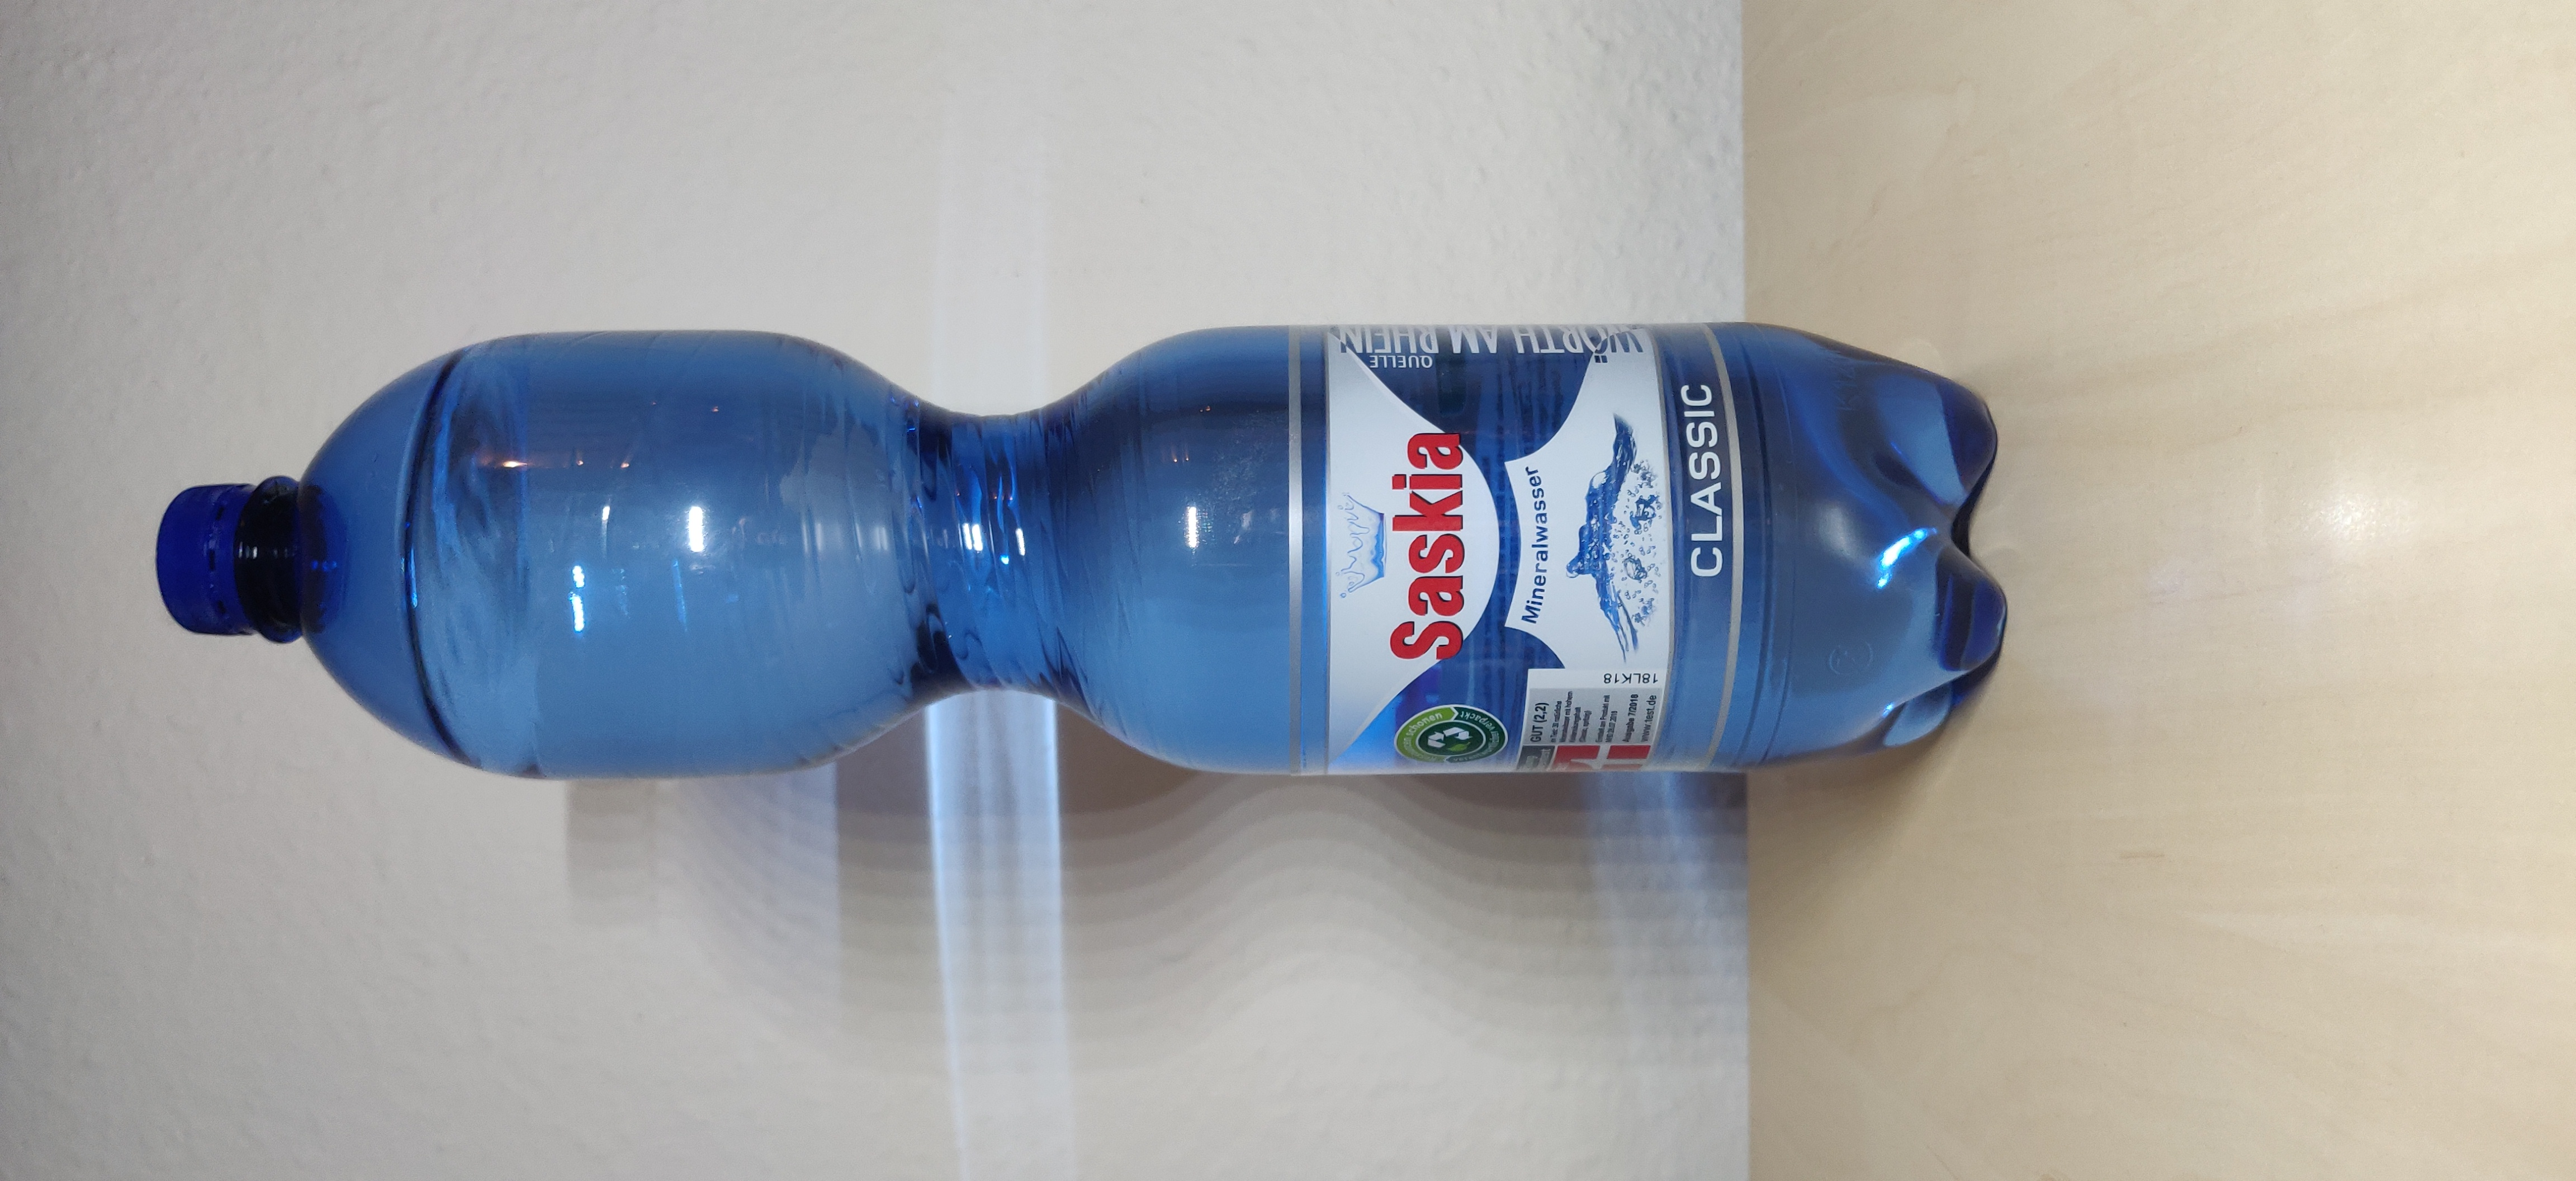
\includegraphics[width=0.32\textwidth]{Bilder/wasser_gross.jpg}}
	\subfigure[Pepsi Cola Klein]{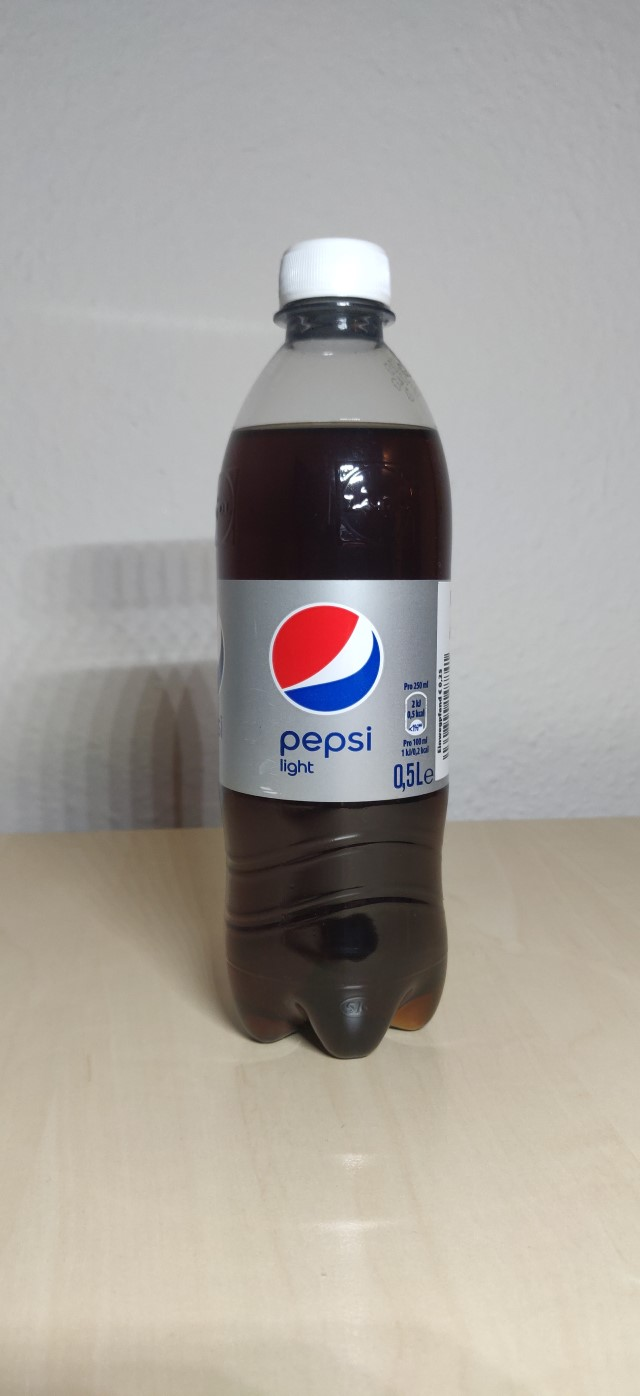
\includegraphics[width=0.32\textwidth]{Bilder/cola_klein.jpg}}
	\subfigure[Pepsi Cola Groß]{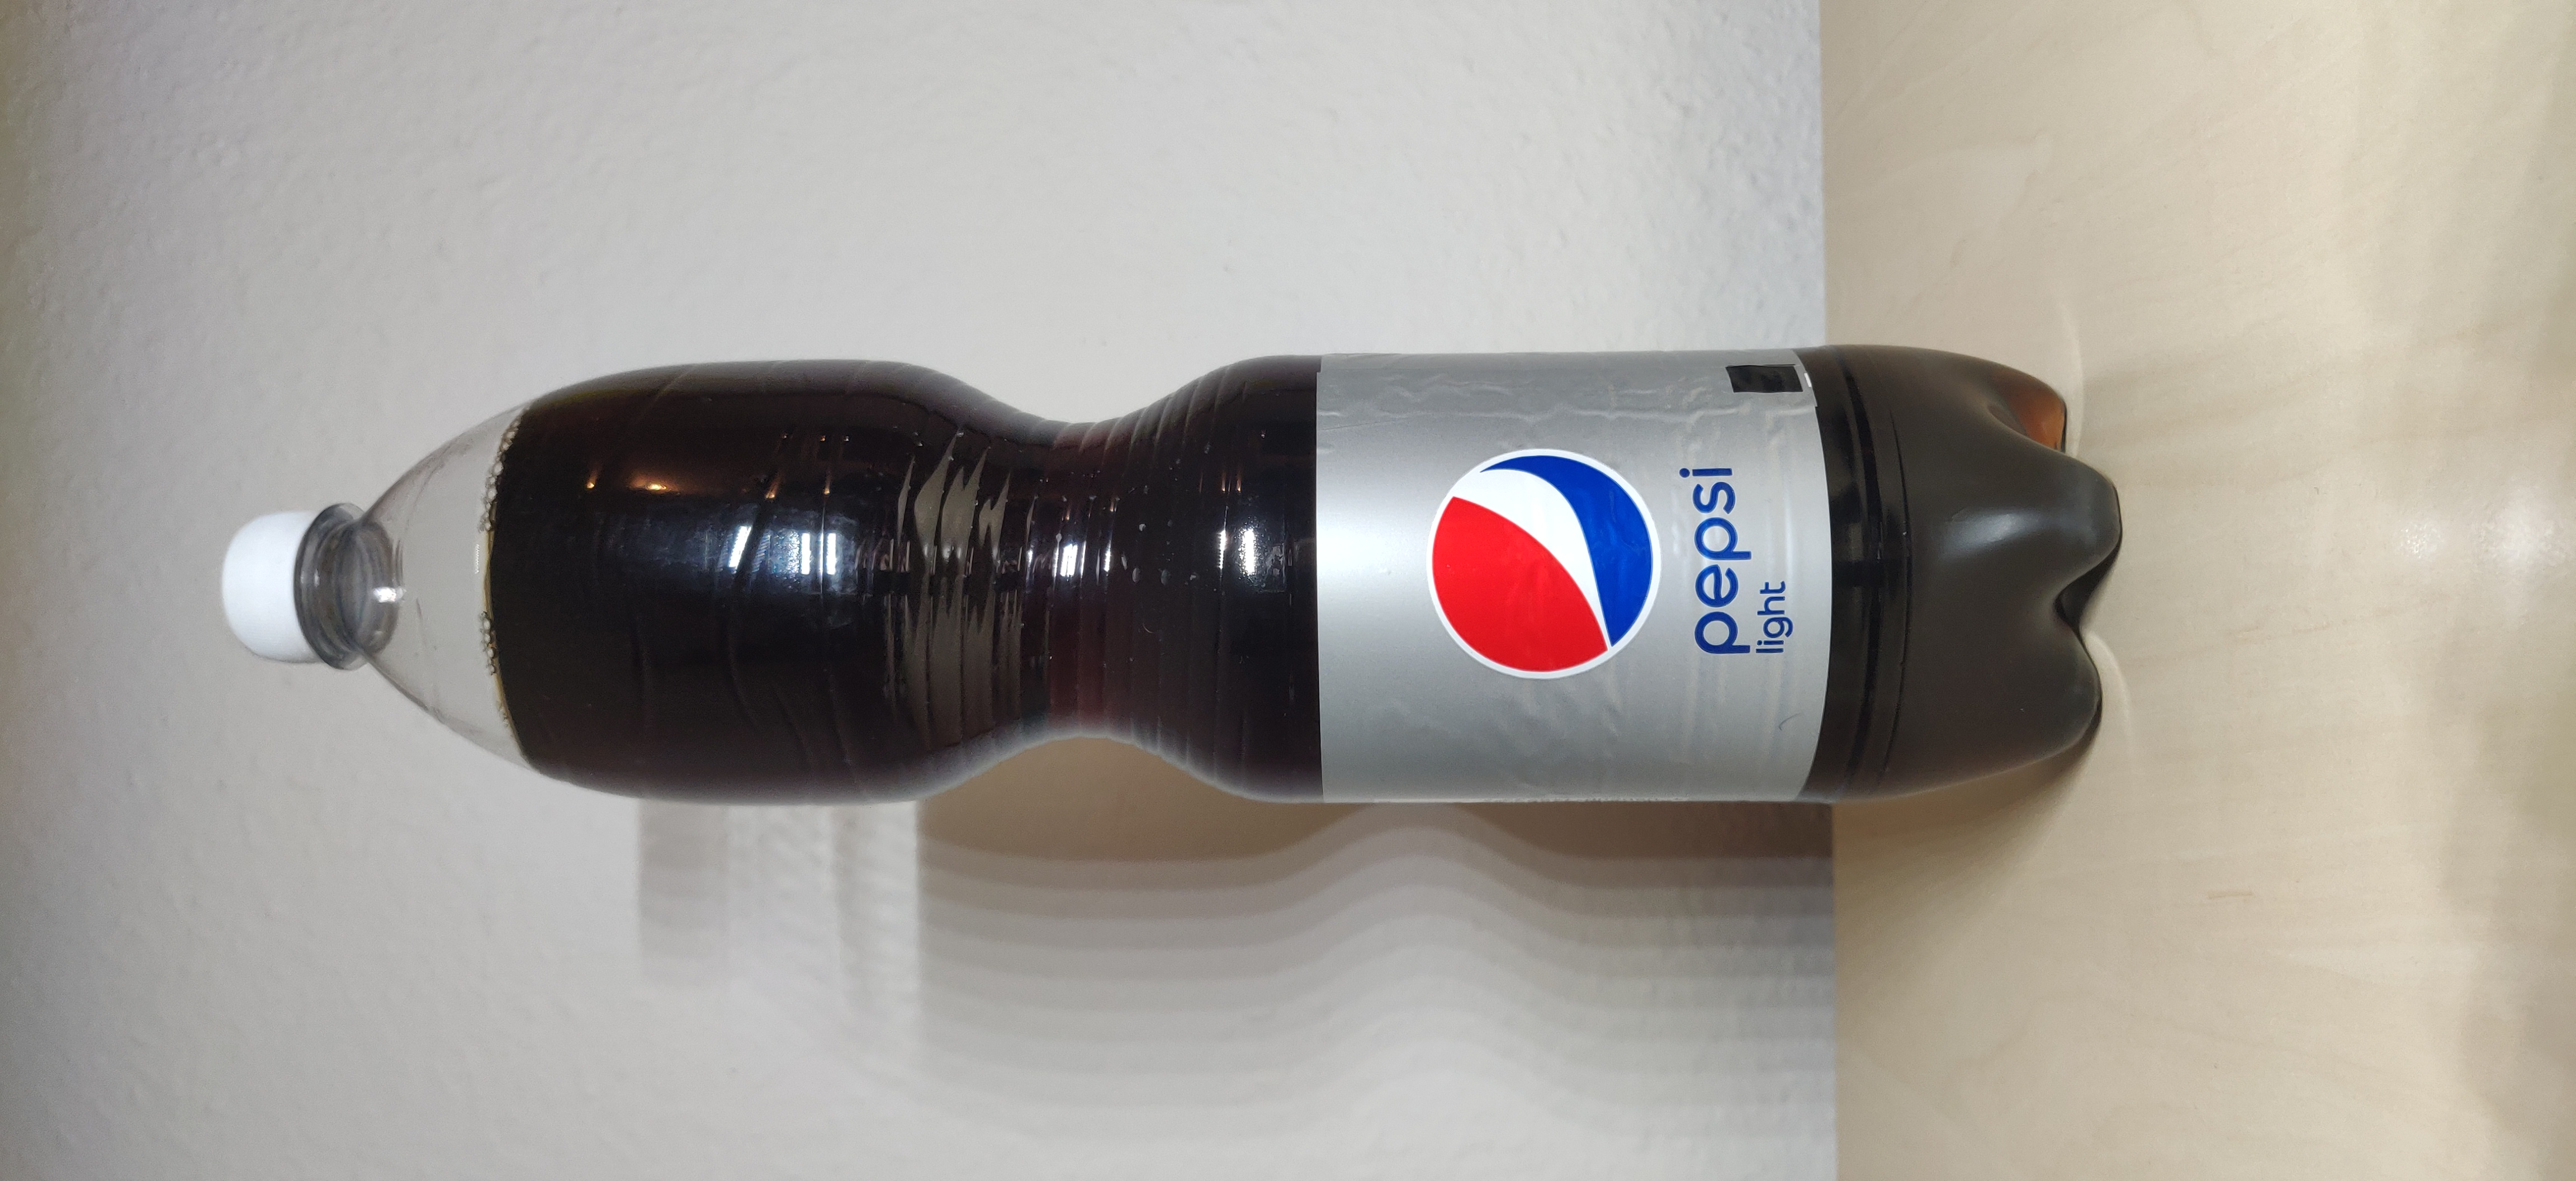
\includegraphics[width=0.32\textwidth]{Bilder/cola_gross.jpg}}
	\subfigure[ISO]{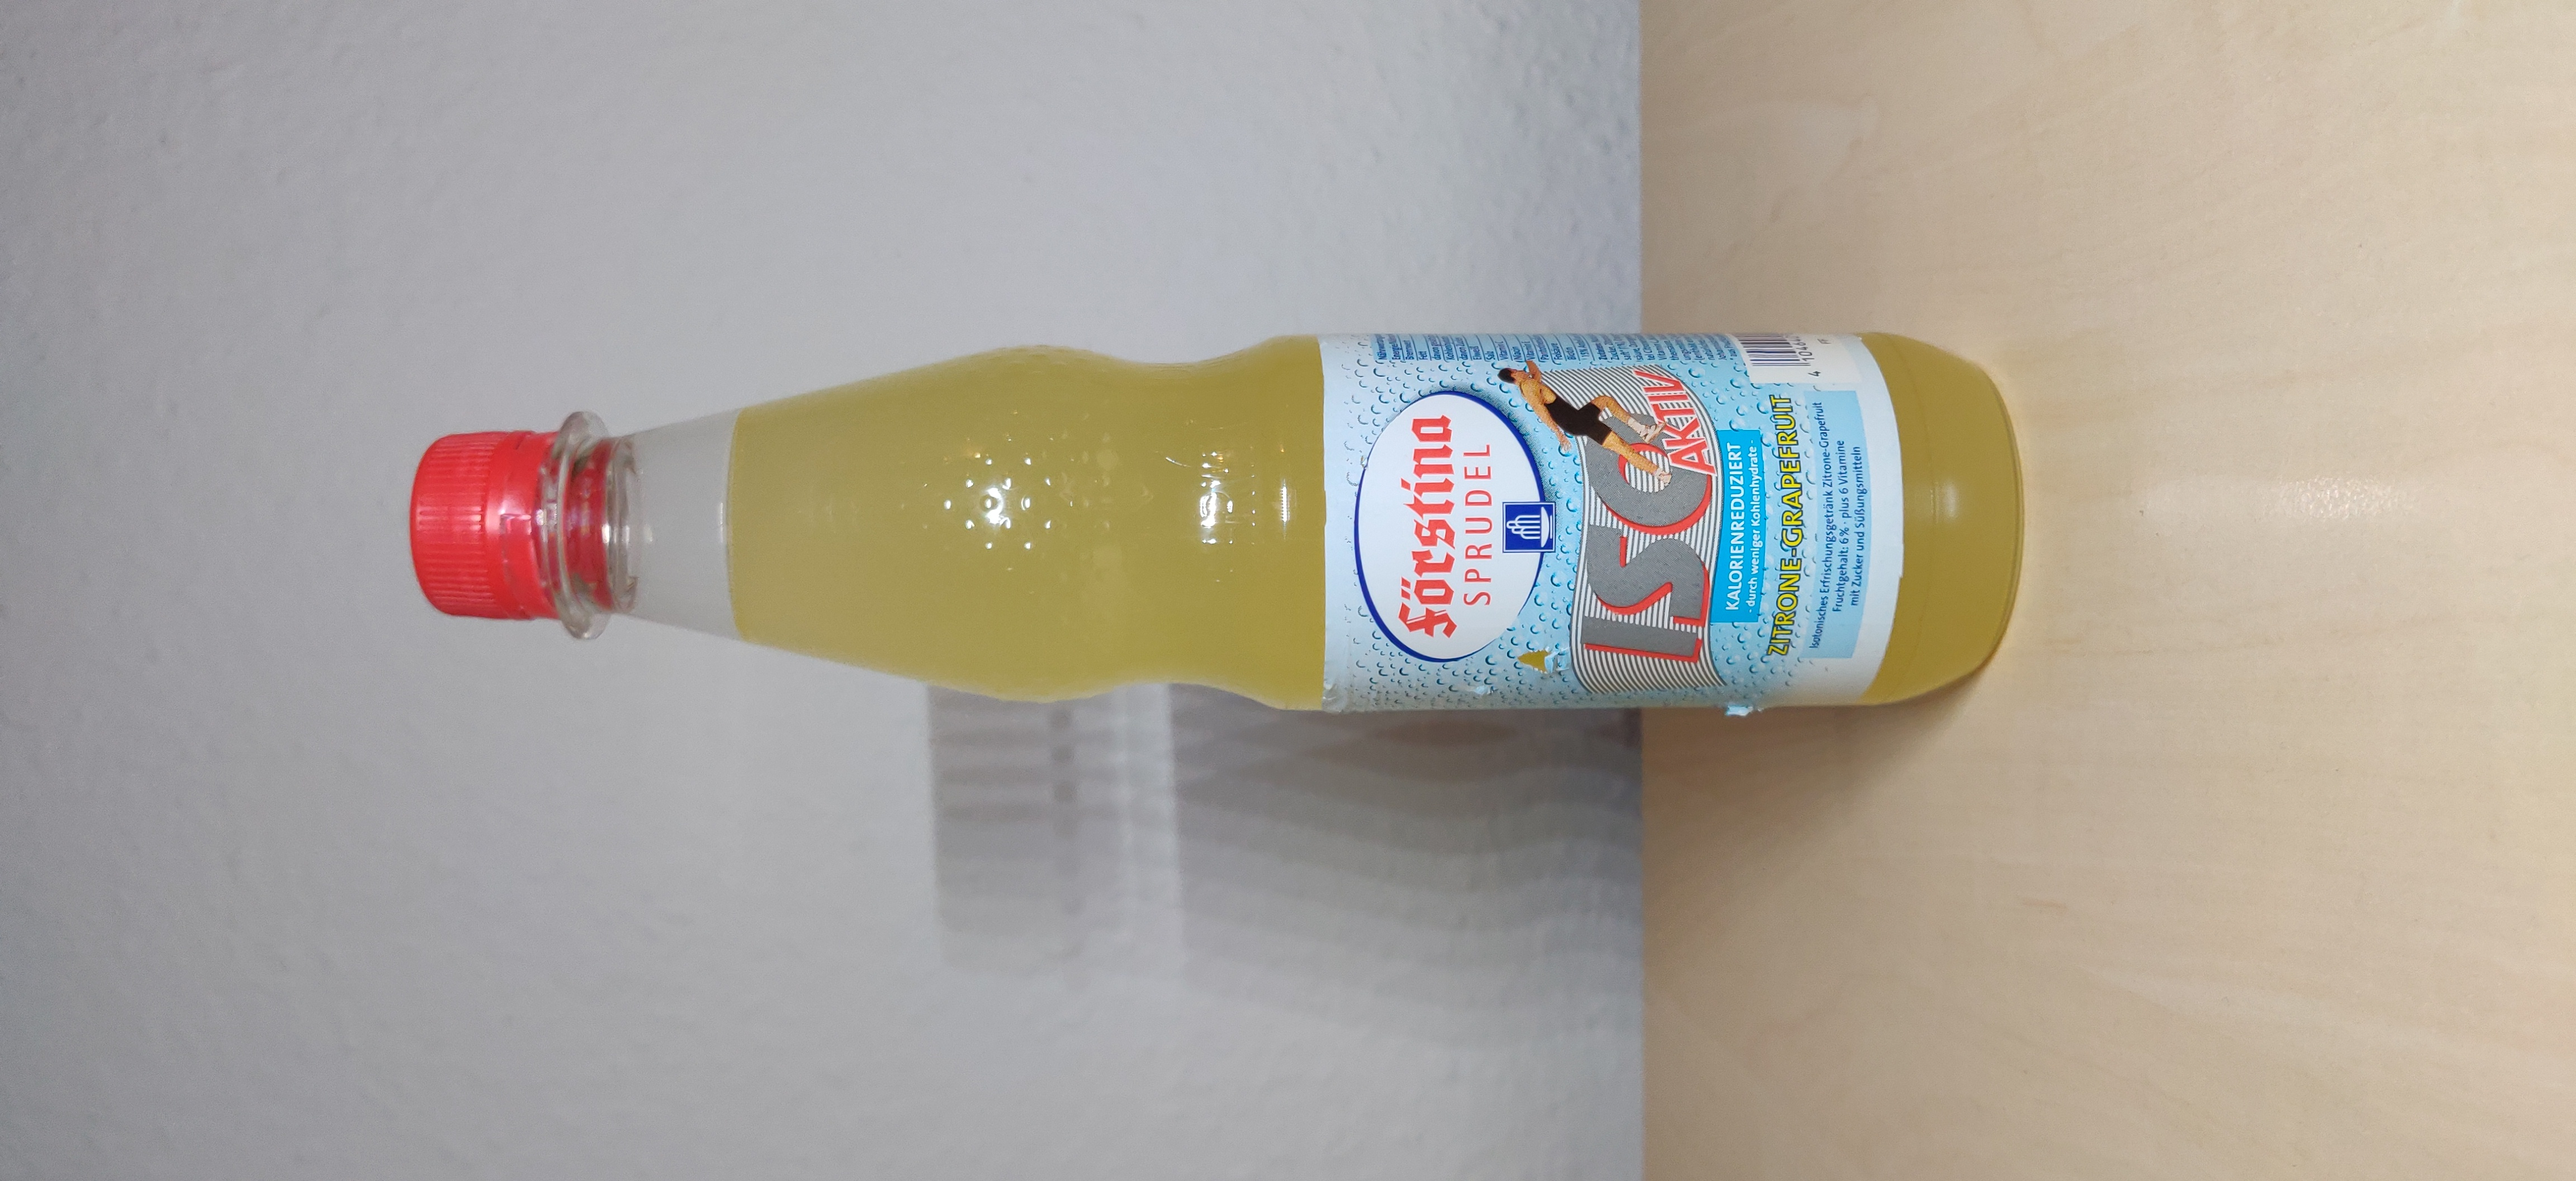
\includegraphics[width=0.32\textwidth]{Bilder/iso.jpg}}
	\subfigure[ACE]{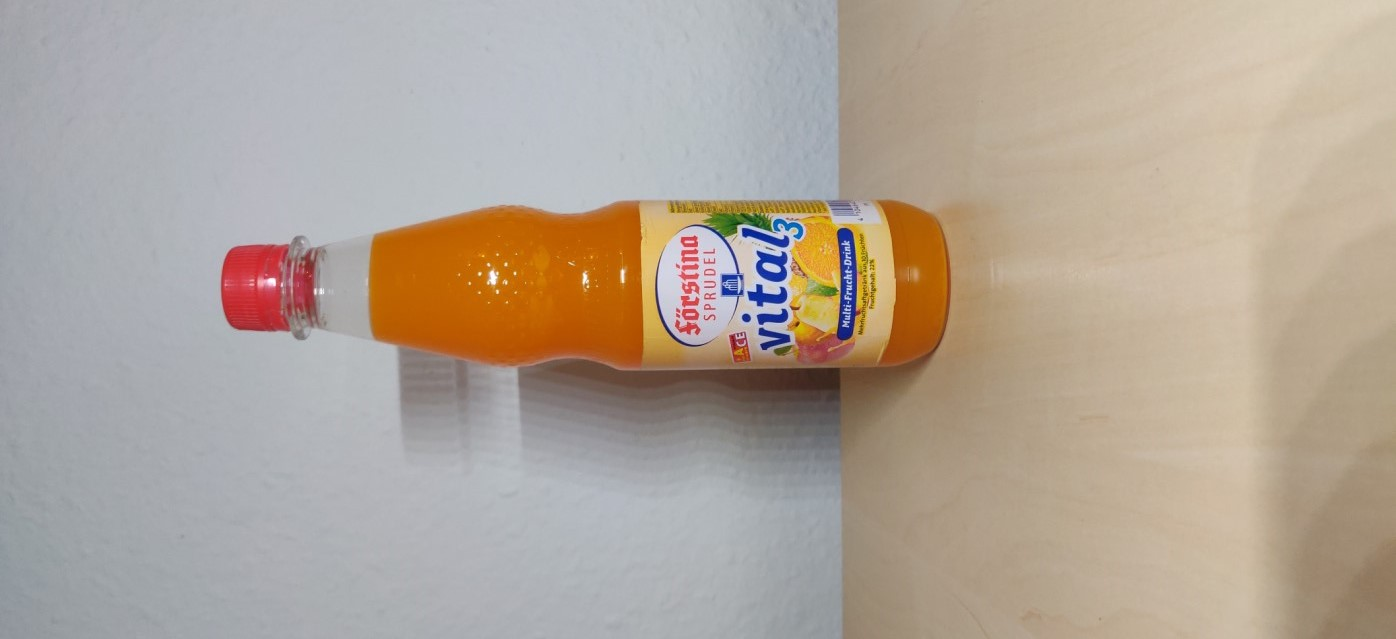
\includegraphics[width=0.32\textwidth]{Bilder/ace.jpg}}
	\subfigure[Stenger Johannisbeerschorle]{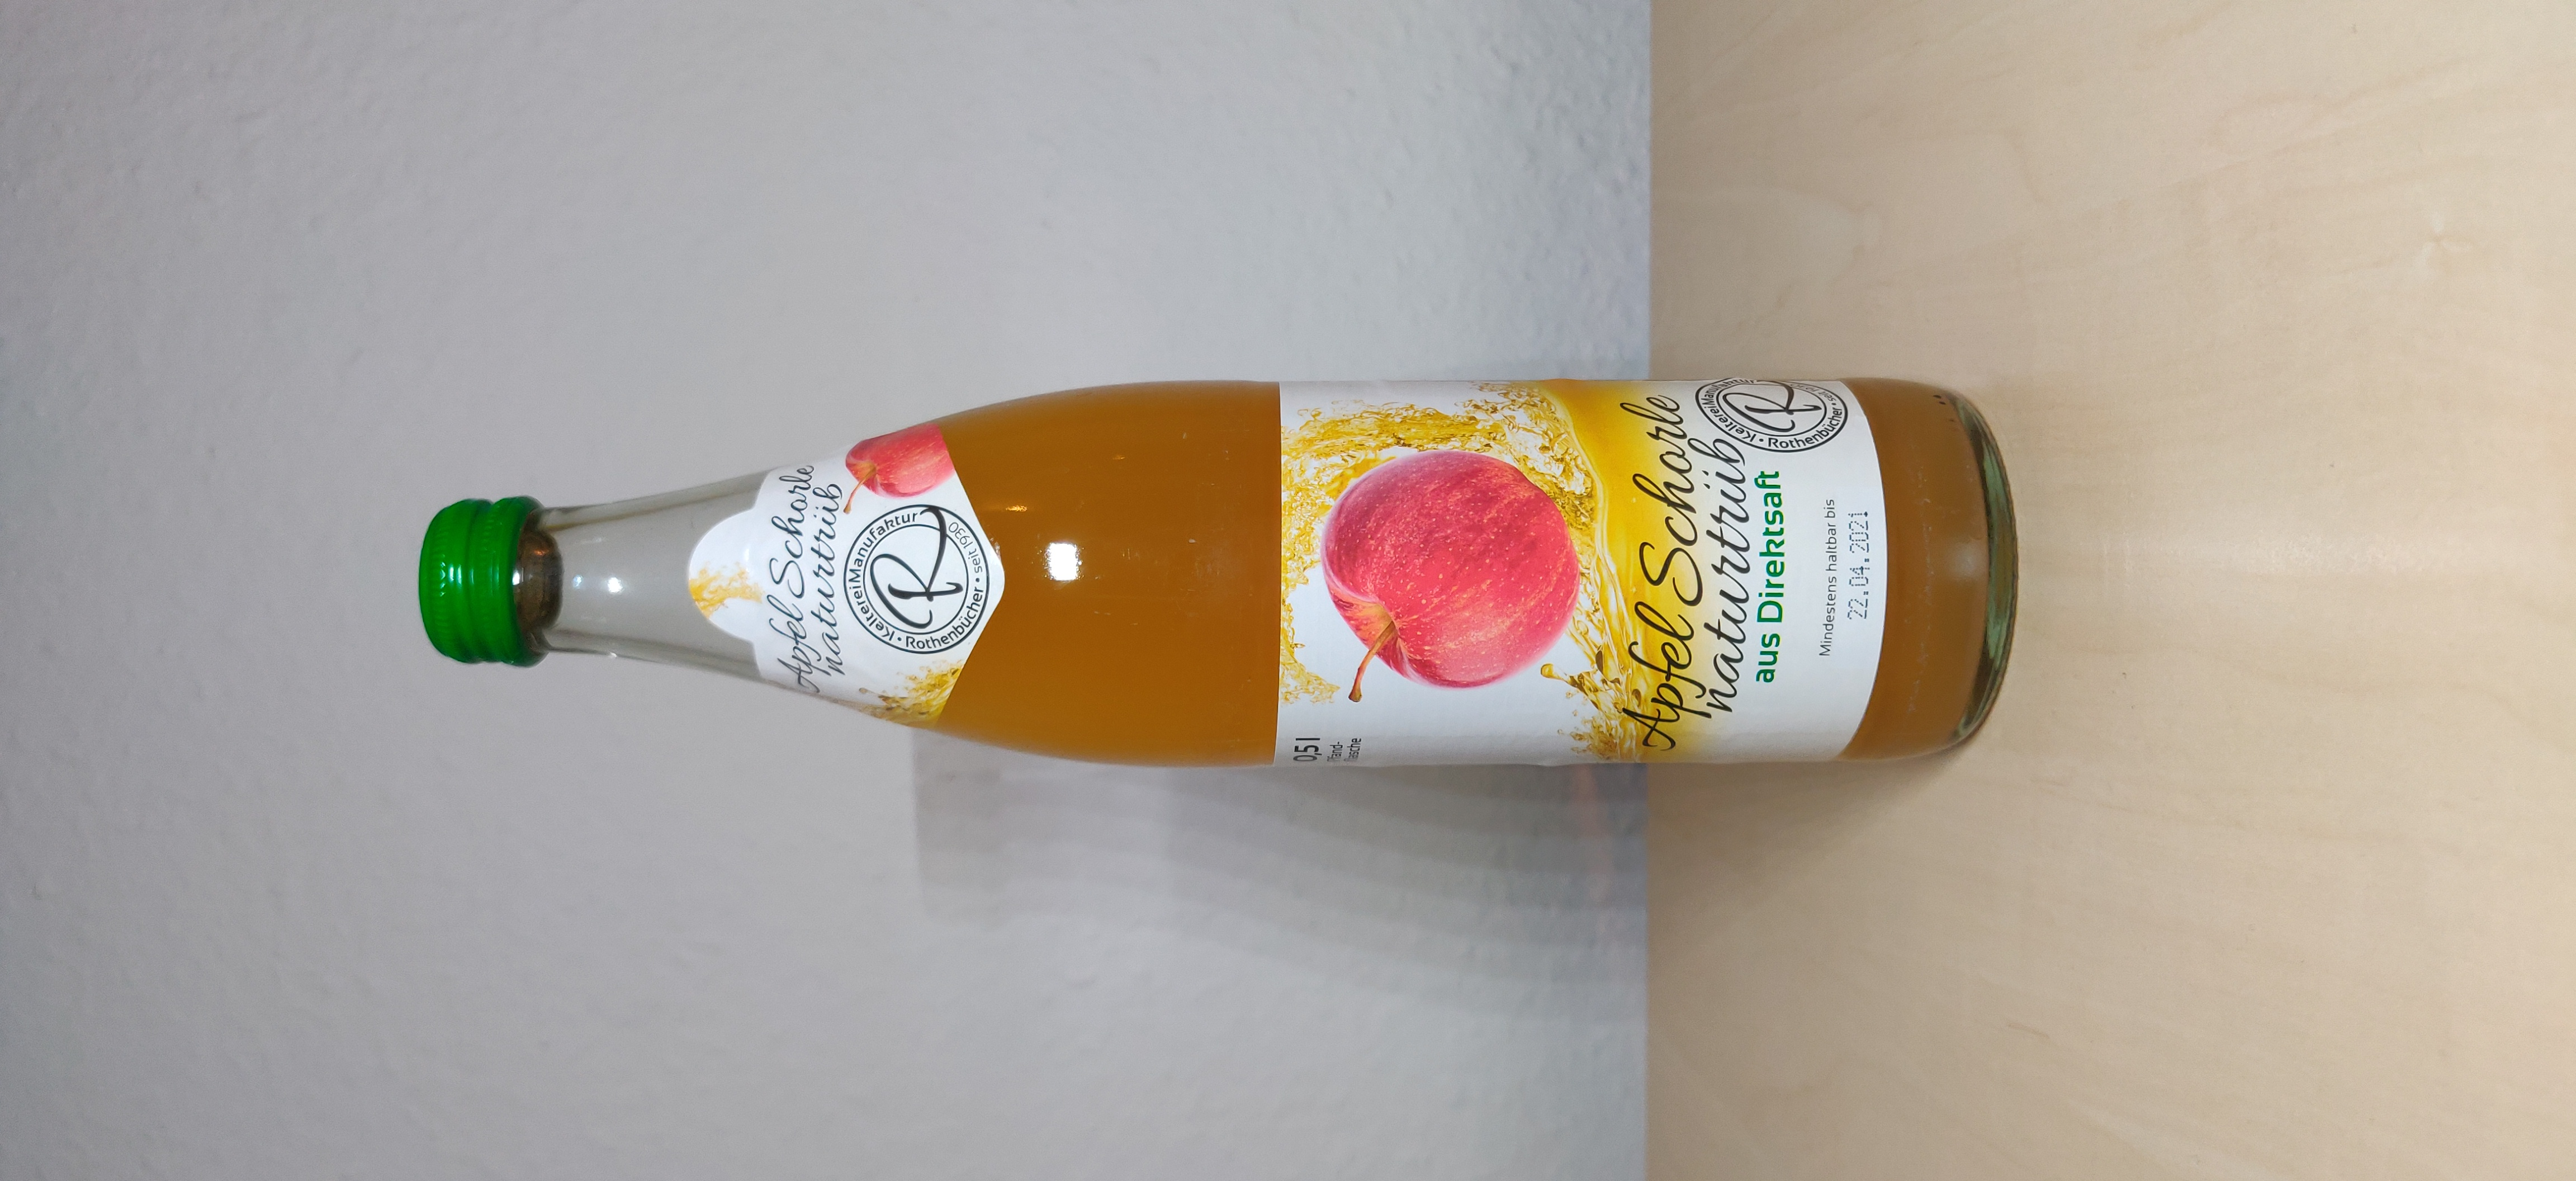
\includegraphics[width=0.32\textwidth]{Bilder/johannisbeerschorle.jpg}}
	\subfigure[Stenger Apfelsaftschorle]{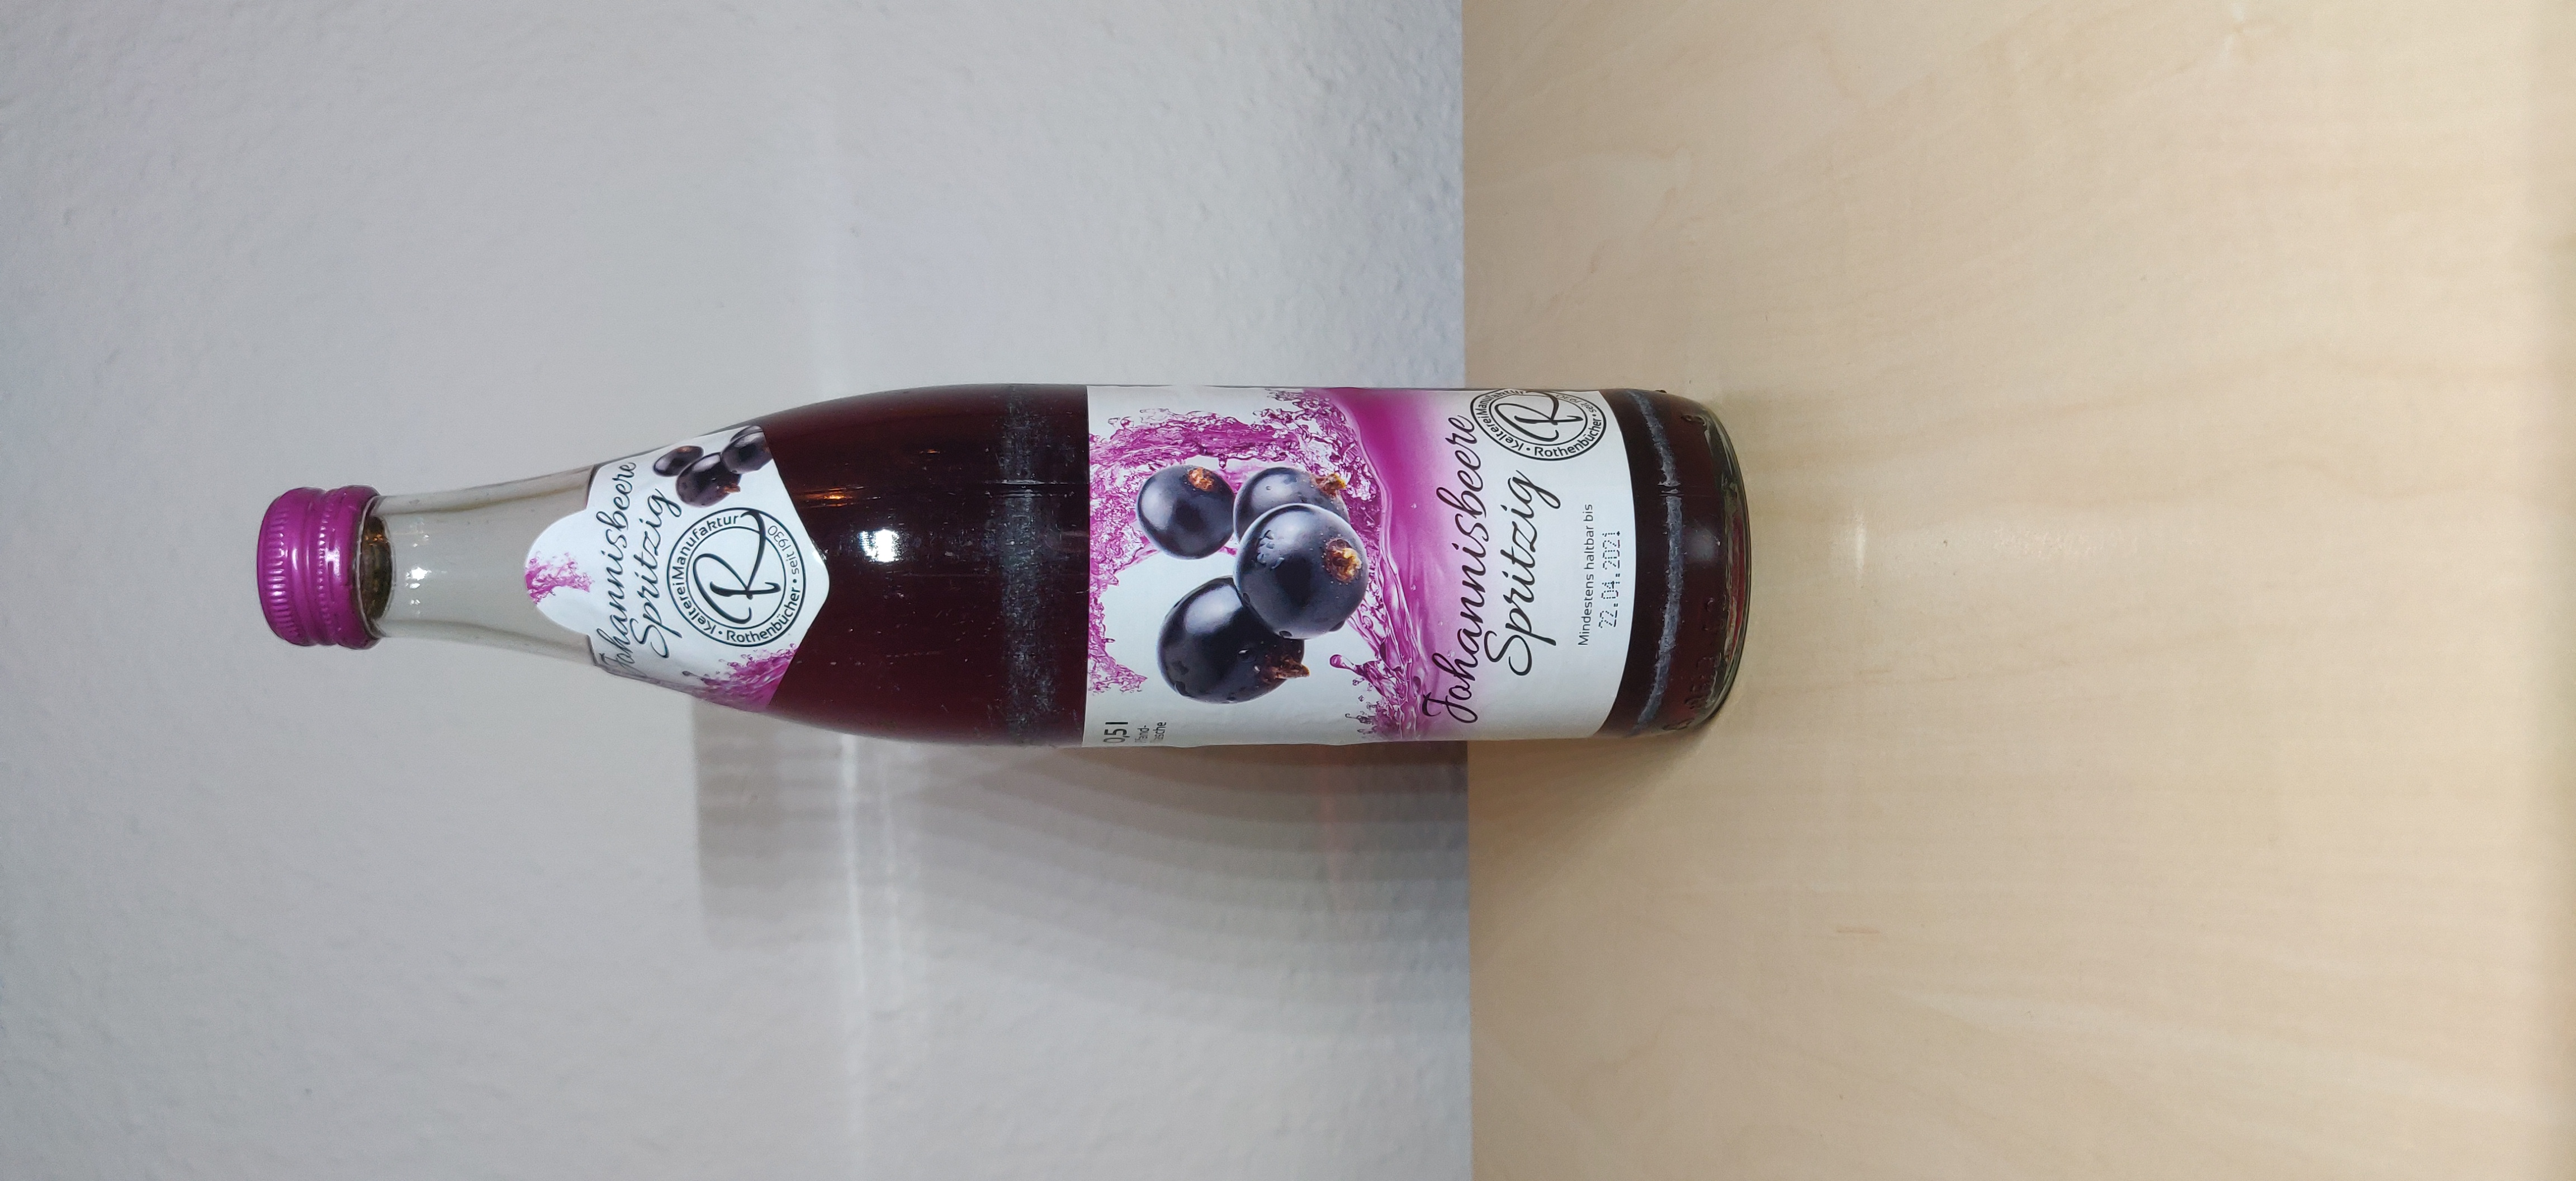
\includegraphics[width=0.32\textwidth]{Bilder/apfelsaftschorle.jpg}}
	\subfigure[Vitamalz Malzbier]{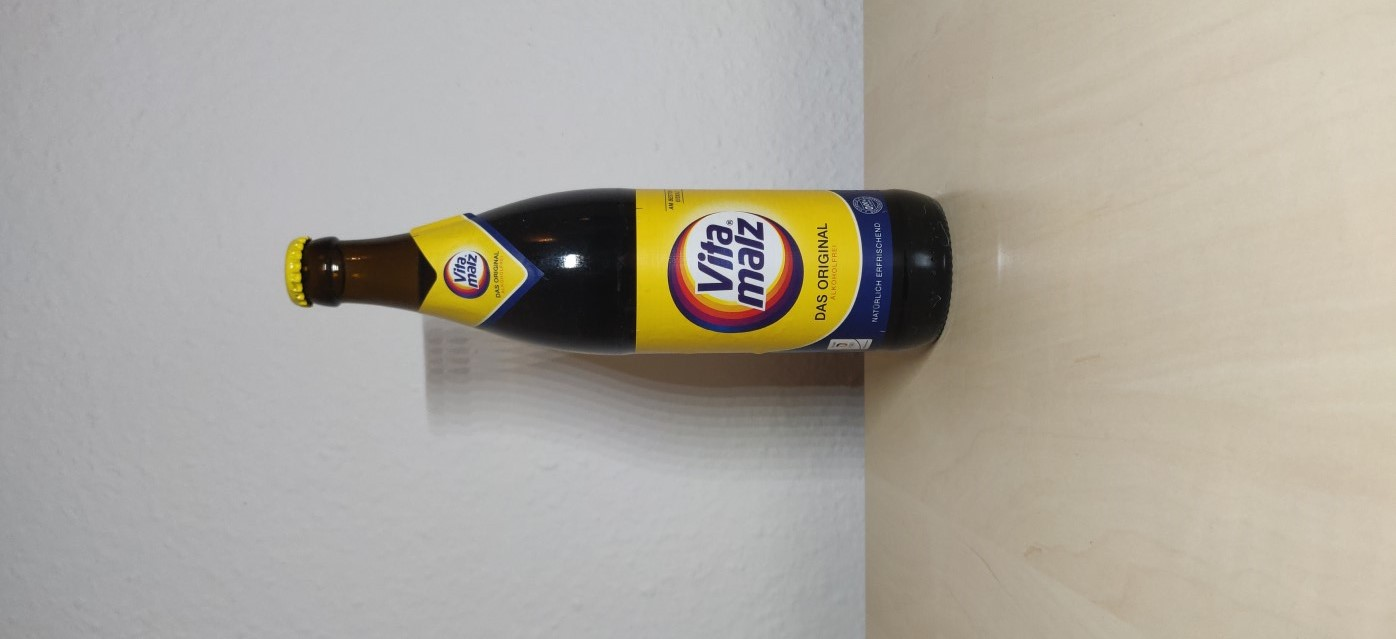
\includegraphics[width=0.32\textwidth]{Bilder/malzbier.jpg}}
	\caption{Die neun Kategorien}
	\label{categories}
\end{figure}

Der Datensatz besteht aus 1000 annotierten Bildern. Die Bilder besitzen eine Auflösung von 2112x4608 Pixels mit einer Farbtiefe von 24 Bit. Alle neuen Kategorien sind nahezu gleichverteilt im Datensatz vorhanden. 

Im initialen Datensatz sind auf 75\% der Bilder die Objekte der jeweiligen Kategorien einzeln und klar erkennbar abgebildet. Hierdurch wird erhofft, dass Modell zunächst auf die Muster der jeweiligen Objekte zu trainieren. In 12,5\% der Bilder sind die Objekte der jeweiligen Kategorien ebenso einzeln, allerdings mit unterschiedlichen Hintergründen, Beleuchtungsverhältnissen, Blickwinkeln und Entfernungen abgebildet. Je nach Umgebung wurden Bilder dieses Anteils als schwer erkennbar markiert. Um das Warenhaus zu simulieren, sind in den letzten 12,5\% der Bilder die Objekte auf Regalen angeordnet, jeweils hintereinander oder in Getränkekästen (siehe Abbildung \ref{regal}). 

\begin{figure}[ht]
	\begin{center}
		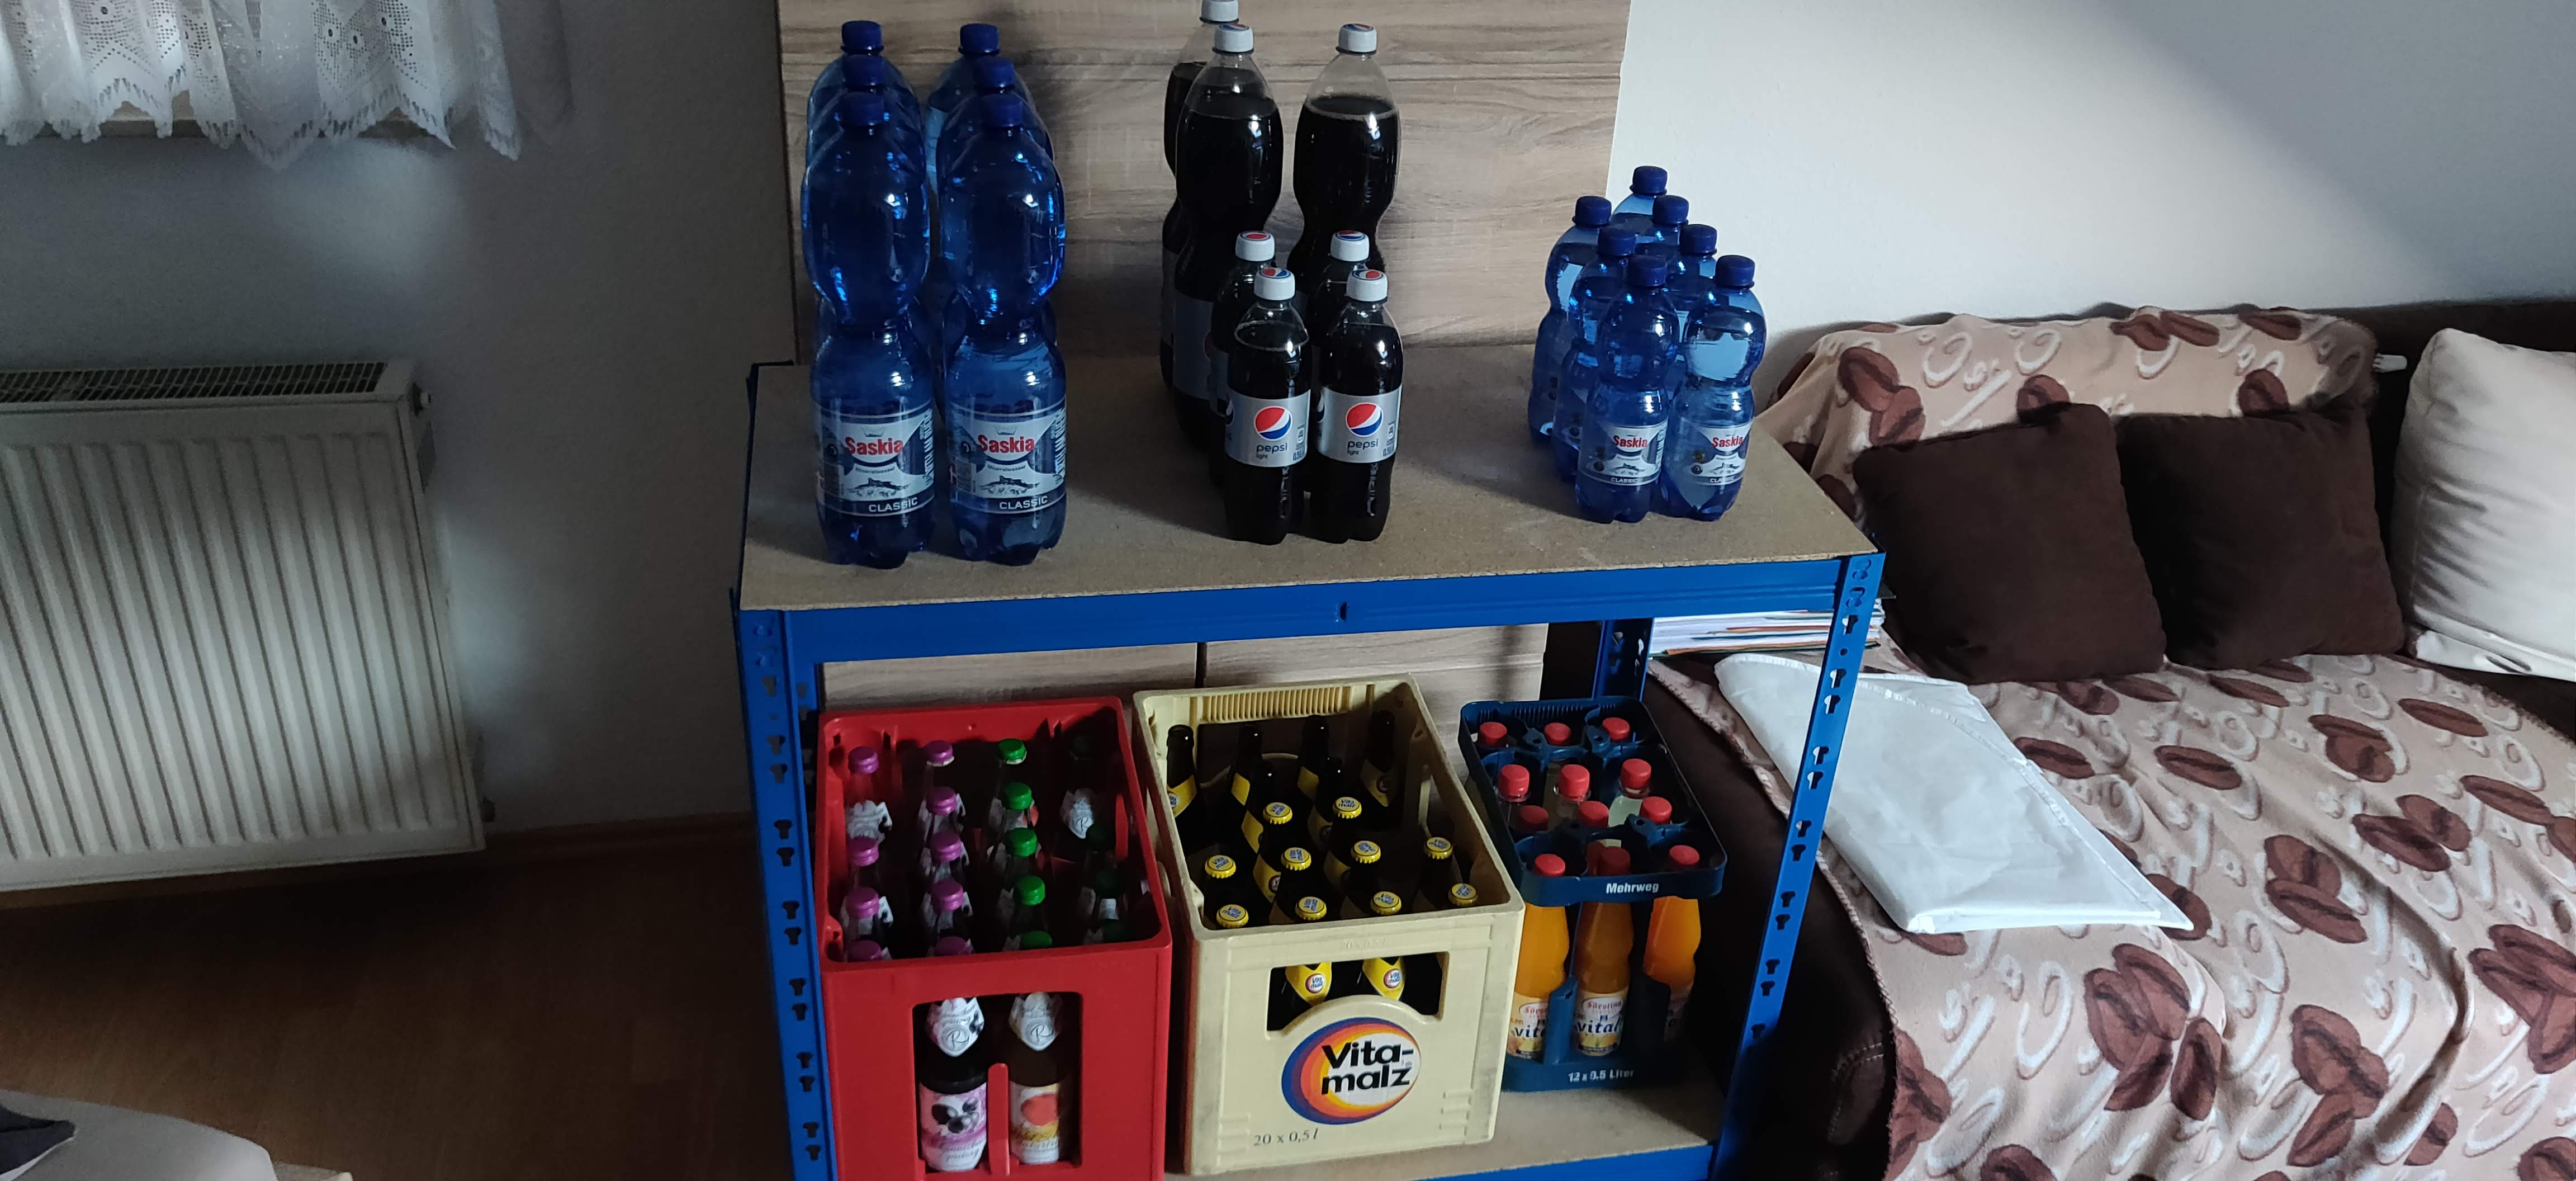
\includegraphics[width=16cm]{Bilder/regal.jpg} 
		\caption[SmartWarehouse Regal]{SmartWarehouse Regal}
		\label{regal}
	\end{center}
\end{figure}


\chapter{Realisierung}

Im folgenden Abschnitt soll auf die Implementierung des \textit{Smart Warehouse} Szenarios eingegangen werden. Insbesondere werden Probleme während der Umsetzung der beiden Objektdetektoren \textit{SSD} und \textit{YOLO} betrachtet, die Realisierung der Dashboard-Webapplikation und des Zählalgorithmus zur Durchführung der Inventur aufgezeigt und letztendlich Herausforderungen im Rahmen der Drohnen Anbindung besprochen.

\section{Umsetzung der Objektdetektoren}

\subsection*{SSD}

Die verwendete Custom-Implementierung in \textit{PyTorch} realisiert die \textit{SSD300} Variante des \textit{SSDs}. Neben kleineren Änderungen in der Codebasis zur Erreichung von Kompatibilität mit aktuellen Bibliotheksversionen und weiteren Anpassungen zur Integration eines eigenen Datenbestandes, wurden vor allem drei größere Erweiterungen durchgeführt. 

Da der erstellte Datenbestand nur 1088 gelabelte Daten enthält, wurde zusätzlich zur Custom-Implementierung ein sechsfaches Kreuzvalidierungsverfahren realisiert. Es dient dazu ein höheres Abstraktionsvermögen des Modells auf dem geringen Datenbestand zu erreichen. Auch unterstützte die Referenzimplementierung keine Validierung durch zuvor ungesehene Daten. Die Modellklassen des Datenbestandes und die Validierungsskripte wurden dahingehend angepasst. Zudem fehlte eine Visualisierung der Entwicklung der Verlustkurven während des Trainingsverfahrens.

Die Referenzimplementierung erstellt sich des Weiteren einige Hilfsdateien, in der die Pfade zu Bildern und weitere Datenstrukturen für Trainingszwecke abgespeichert werden. Ohne diese ist kein Training möglich, das Trainingsskript fordert demnach Zugriff auf den Sekundärspeicher. 

Um ein lokales Training auf der \textit{NVIDIA GeForce GTX 1080} GPU zu ermöglichen, wurde zudem \textit{CUDA} Version 10.1 verwendet. Trainiert wurde mit folgenden Hyperparametern:
\begin{itemize}
	\item Batchgröße: 16
	\item Lernrate: $1.0\cdot 10^{-3}$
	\item Momentum: 0.9
	\item Kreuzvalidierungen: 6 à 22 Epochen
	\item Epochen: 132
	\item Gradientenverfahren: Stochastic Gradient Descent
	\item Kostenfunktion: Smooth L1
\end{itemize}

Das Basisnetzwerk des \textit{SSDs} besteht aus einem auf \textit{ImageNet} vortrainierten \textit{VGG16}. Die restlichen \textit{Convolutional Layer} sind \textit{Xavier} initialisiert. 

Die Hyperparameter sind nahezu gleich zu denen in der ursprünglichen wissenschaftlichen Veröffentlichung. Die Batch Größe im \textit{Mini-Batch} Verfahren wurde für größere Stabilität von 32 auf 16 heruntergesetzt. Auch in der Evaluierung wurde die Batch Größe von 64 auf 48 verkleinert, da die Eingangsdaten eine weitaus höhere Auflösung als die ursprünglich im \textit{PascalVOC} verwendeten Daten haben. Andernfalls wird Gefahr gelaufen, einen Speicherüberlauf zu verursachen. Der Datensatz wurde in fünf Untermengen unterteilt, in jedem Kreuzvalidierungsschritt diente jeweils eine Untermenge als Testdatensatz.

\subsection*{YOLO}

Für \textit{YOLO} wurde die neuste Version \textit{YOLOv3} implementiert. Hierbei kommt das \textit{Dark-""net} Framework zum Einsatz, eine Implementierung in C. Vor der initialen Kompilierung müssen einige Konfigurationsschritte unternommen werden, weil auch der Betrieb auf einer normalen CPU oder einer GPU mit Tensor Kernen möglich ist. Für das Training kommt eine \textit{NVIDIA GeForce RTX 2060 SUPER} GPU zum Einsatz, deren enthaltenen Tensor Kerne mitbenutzt werden. Die benötigten Hyperparameter wurden dabei wie folgt gesetzt:

\begin{itemize}
	\item Batchgröße: 64
	\item Subdivisions: 16
	\item Lernrate: $1.0\cdot 10^{-3}$
	\item Momentum: 0.9
	\item Maximale Anzahl Batches: 18000
\end{itemize}

Im Unterschied zum \textit{SSD} kann \textit{YOLO} die in den GPU Speicher zu ladende Datenmenge eines Batches durch sogenannte \textit{Subdivisions} festgelegt. Hierbei werden nur noch $Batchgroesse \div Subdivisions$ Bilder gleichzeitig in die GPU geladen, um einen Speicherüberlauf zu vermeiden.

Die Lernrate sowie das Momentum bleiben wie in der Dokumentation empfohlen unverändert zu den Referenzwerten. Im Gegensatz zu \textit{SSD} wird kein Maximum für die Anzahl an Epochen, sondern ein Maximalwert für die zu durchlaufenen Batches gesetzt. Dieser Wert wird abhängig von der Menge an gelabelten Klassen gesetzt und kann als Empfehlung aus der Dokumentation für das \textit{Darknet} Framework entnommen werden. 

\section{Dashboard Entwicklung}

Der Server wurde mit dem \textit{Flask} Framework in Python implementiert und läuft auf dem \textit{Web Server Gateway Interface} (WSGI) server \textit{Waitress}. Er führt den Inferenzalgorithmus des \textit{SSDs} bzw. des \textit{YOLO} Objektdetektors für jeden Frame des empfangenen Videostreams der Drohne aus und streamt die inferierten Bilder mit den Bounding Boxen an jeden Client. Der Client wurde mit dem \textit{Bootstrap} Framework grafisch gestaltet (siehe Abbildung \ref{webapp}).

\begin{figure}[H]
	\begin{center}
		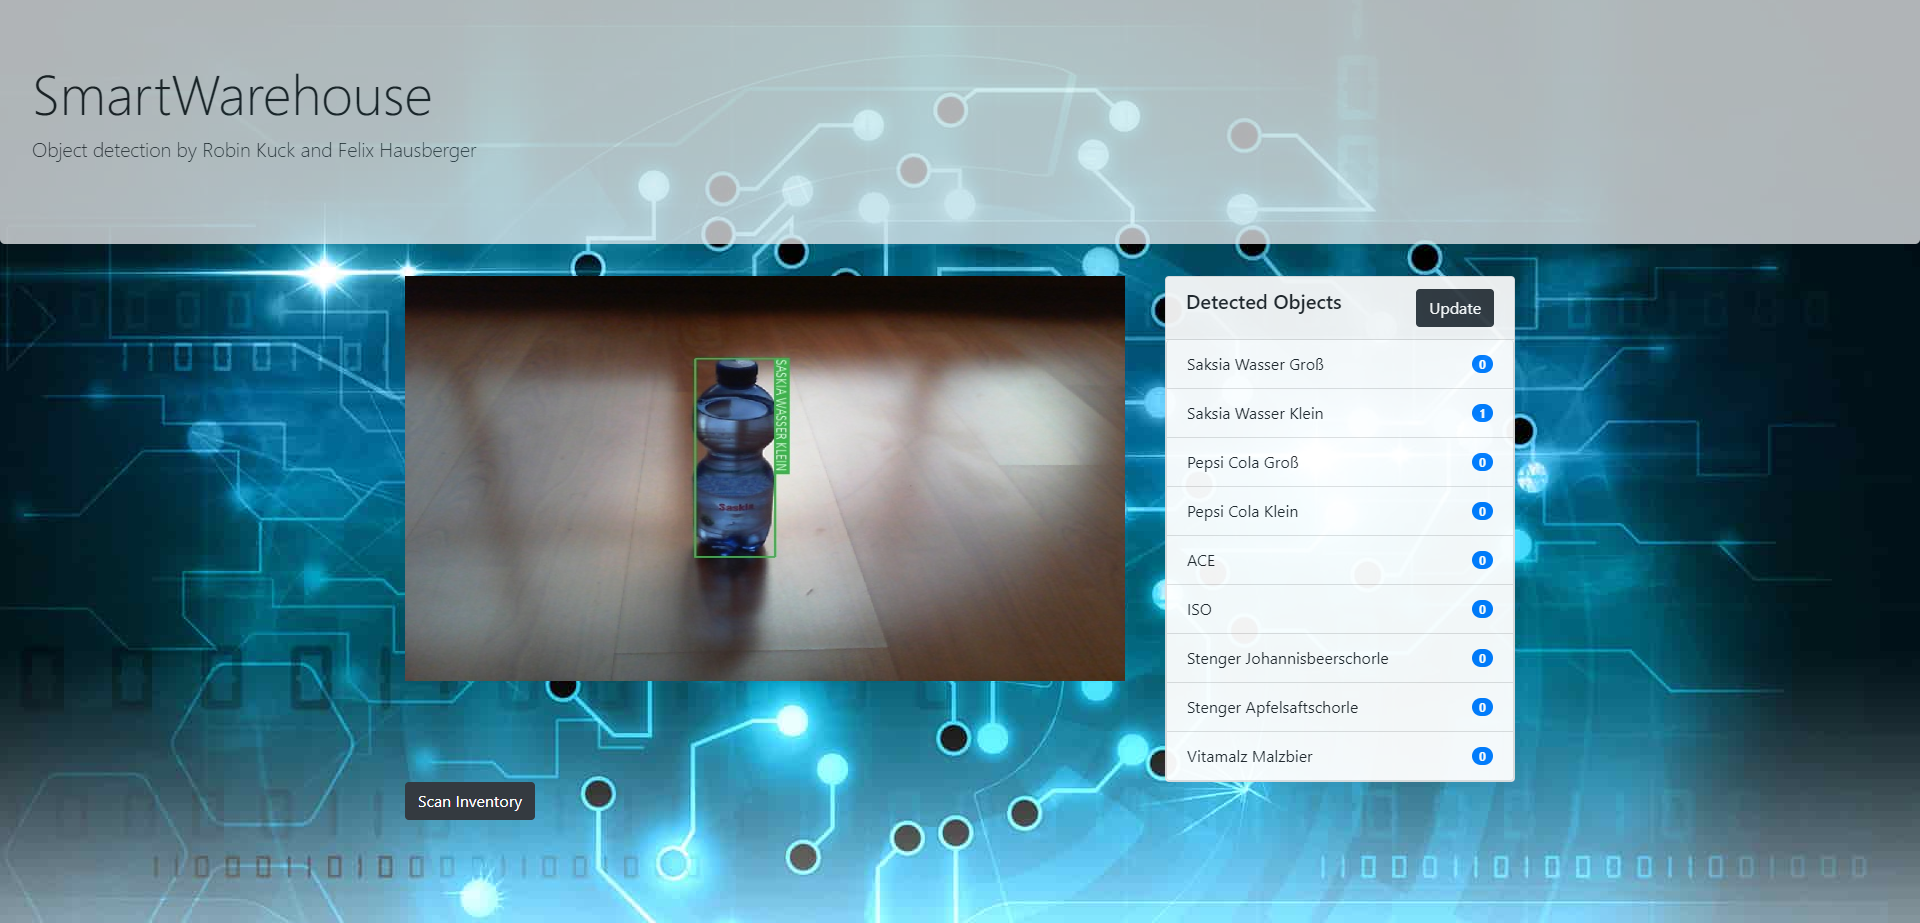
\includegraphics[width=15cm]{Bilder/webapp.jpeg} 
		\caption[Webapplikation SmartWarehouse]{Webapplikation SmartWarehouse}
		\label{webapp}
	\end{center}
\end{figure}

Auf Anfrage eines Client kann dieser die aktuell gezählten Objekte vom Server abfragen. Der Zählalgorithmus wird im folgenden Unterkapitel erklärt. 

\section{Zählalgorithmus}

\lstinputlisting[
label={code:formfield},
caption={Zählalgorithmus zum Zählen der detektierten Objekte},
captionpos=b,
basicstyle=\ttfamily\scriptsize,   
firstline=1,              
lastline=11                 
]{Quellcode/algorithmus.txt}

Der Algorithmus \ref{code:formfield} wird momentan dazu verwendet, um für das Industrieszenario einer Inventur einzelne detektierte Objekte zu zählen. Nach jedem Inferenzvorgang werden die detektierten Objekte abgespeichert, sodass der Algorithmus bei Aufruf sowohl auf die zuletzt detektierten Objekte \textit{o\_alt}, als auch auf die neu detektierten Objekte \textit{o\_neu} zugreifen kann. Für alle detektierten Objekte im aktuellen Durchlauf durchsucht er alle zuletzt detektierten Objekte, um herauszufinden, ob ein Objekt bereits im vorherigen Bild vorhanden war. Ausschlaggebend hierfür ist das gleiche \textit{Label} als auch die Distanz der Bounding Boxen des aktuell detektierten Objekts zum Objekt der Vorrunde. Nur falls das Objekt nach diesen Kriterien nicht bereits in der Vorrunde vorhanden war, wird es gezählt. Das Problem, das der Algorithmus zu lösen versucht, enthält allerdings eine weitere Komplexitätsstufe. Dasselbe Objekt kann im Laufe der Inventur erneut auftreten und dessen relative Position im Bild ist ebenso variabel. In diesem Falle werden Objekte doppelt gezählt. 

\section{Drohnen Anbindung}

\subsection*{Flugsequenz}
Wie in Kapitel \ref{drone_selection} beschrieben wird das Versenden von Befehlen mittels einer bidirektionalen Verbindung realisiert. Die Kommunikation durch eine Socket\footnote{Mit Sockets können Daten bidirektional zwischen  Programmen ausgetauscht werden, die entweder auf dem gleichen oder auf einem anderen durch eine Netzwerkadresse erreichbaren PC laufen.} Verbindung ist dabei eine passende Lösung. Python bietet ein \textit{socket} Modul an, welches verschiedene Typen von Sockets unterstützt. Das nachfolgende Listing zeigt die Initialisierung einer Instanz der Socket Klasse:

\lstinputlisting[
label={code:python},
caption={Initialisierung der Socket Klasse},
captionpos=b,
basicstyle=\ttfamily\scriptsize,   
firstline=1,              
lastline=2                 
]{Quellcode/socket_init.py}

Die Methode \textit{socket()} erzeugt eine neue Instanz der Socket Klasse und benötigt zwei Parameter für die Adressfamilie und den Verbindungstyp. \textit{AF\_INET} steht für Internet-Socket-Adresse, die sich aus IP-Adresse und Portnummer zusammensetzt. Der Parameter \textit{SOCK\_DGRAM} gibt an, dass die Socket Verbindung über das UDP-Protokoll aufgebaut wird. Für das Empfangen von Daten wird die Instanz zusätzlich an eine Adresse (hier \textit{localhost:9000}) gebunden.

Im folgenden Listing wird jeweils die Methode zum Senden von Befehlen und Empfangen von Antworten gezeigt:

\lstinputlisting[
label={code:python},
caption={Methode für das Versenden von Befehlen und Empfangen von Antworten},
captionpos=b,
basicstyle=\ttfamily\scriptsize,   
firstline=1,              
lastline=22                 
]{Quellcode/socket_send_command.py}

Die Methode \textit{send\_command()} erhält beim Aufruf den auszuführenden Befehl als Parameter vom Typ \textit{String}. Für jeden Befehl wird eine neue Instanz der Klasse \textit{Stats} in das \textit{log} Array einfügt. Die Klasse \textit{Stats} dient für die Datenhaltung eines gesendeten Befehls und die entweder noch ausstehende oder bereits erfolgte Antwort. Daraufhin wird der Befehl mit Hilfe der Methode \textit{socket.sendto()} an den Socket übermittelt. Dieser erhält neben dem Befehl auch die Zieladresse, die als Tupel bestehend aus IP-Adresse und Port übergeben wird. Im nächsten Schritt wird mittels einer Schleife auf das Erreichen der Antwort gewartet. Dabei wird die seit dem Versand der Nachricht vergangene Zeit berechnet und wenn diese größer als die auf 15 Sekunden festgelegte Konstante \textit{MAX\_TIME\_OUT} ist, gibt die Methode \textit{False} zurück. Sobald jedoch eine Antwort empfangen wurde, kann die Schleife übersprungen und \textit{True} zurückgegeben werden.

Aufgrund der UDP basierten Verbindung ist nicht garantiert, ob und in welcher Reihenfolge Antworten empfangen werden können. Um dem entgegenzuwirken, kommt die Methode \textit{receive\_thread()} zum Einsatz, die in einem parallel laufenden Thread ausgeführt wird und die empfangene Antwort immer dem zuletzt geschickten Befehl zuordnet. Durch die Zuweisung wird die zuvor beschriebene Blockierung durch die Schleife in der Methode \textit{send\_command()} aufgehoben. 

Mit diesen zwei Methoden wird ein synchroner Versand der Befehle möglich, bei dem immer nur dann ein neuer Befehl geschickt wird, wenn bereits eine Antwort auf den vorherigen empfangen oder ein Timeout erkannt wurde. In der Flugsequenz fliegt die Drohne zunächst nah vor einem Regal mit zwei Böden her, um alle Objekte aus der Nahaufnahme detektieren zu können. Danach fliegt die Drohne zurück, um das gesamte Regal im Blickwinkel zu haben. Die finale Befehlskette sieht wie folgt aus:

\begin{itemize}
	\item Command (Übernahme der Steuerung)
	\item streamon (Einschalten von Video Stream)
	\item up 150 (Aufsteigen um 150 cm)
	\item right 100 (Nach rechts fliegen um 100 cm)
	\item down 100 (Absteigen um 100 cm)
	\item left 100 (Nach links fliegen um 100 cm)
	\item up 100 (Nach oben fliegen um 100 cm)
	\item right 50 (Nach rechts fliegen um 50 cm)
	\item back 150 (Nach hinten fliegen um 150 cm)
	\item streamoff (Ausschalten von Video Stream)
	\item land (Landung)
\end{itemize}

\subsection*{Modellinferenz}

Der Video Stream der Drohne kann auf dem zentralen Server mittels der \textit{openCV} Klasse \textit{VideoCapture} in Python über das UDP Protokoll angesprochen werden. Anschließend kann jeder Frame des Streams einzeln durch \textit{SSD} inferiert werden.

Da das \textit{Darknet} Framework für \textit{YOLO} allerdings wie zuvor angemerkt in C implementiert ist, kann keine nahtlose Inferenz auf dem Python Server wie bei \textit{SSD} umgesetzt werden. Hierfür muss auf die Kompilierung einer \textit{Dynamic Link Library} (DLL) zurückgegriffen werden. Eine \textit{DLL} ist eine ausführbare Datei, die Funktionen und Ressourcen als geteilte Bibliothek bereitstellt. Programme, die in verschiedenen Programmiersprachen implementiert wurden, können dadurch die gleiche DLL-Funktion aufrufen und die Inferenz mit \textit{YOLO} kann somit durch das Python Programm aufgerufen werden \cite{MicrosoftCorporation.27.01.2020}.


\chapter{Ergebnisse} \label{evaluation}

In diesem Kapitel werden die Ergebnisse des Trainings und des Einsatzes der Objektdetektoren nach den in Kapitel \ref{eval} definierten Kriterien dargestellt. Es beinhaltet die Ergebnisse zur Präzision, zum Inferenzverhalten, zum Reaktionsvermögen und zum Trainingsverhalten der Detektoren.

\section{Präzision und Inferenzverhalten}

\subsection*{SSD}

Ursprünglich wurden 500 Epochen für das Training vorgesehen. Da allerdings beim Training schon nach knapp über hundert Epochen sich der Gradient der Kostenfunktion nur träge veränderte, wurde im Sinne des \textit{Early Stoppings} nach 121 Epochen das Training vorzeitig beendet, um \textit{Overfitting} zu vermeiden. Abbildung \ref{ssdloss} zeigt den Verlauf der Trainingsverlustkurve und der Testverlustkurve während des Kreuzvalidierungsverfahrens.

\begin{figure}[H]
	\begin{center}
		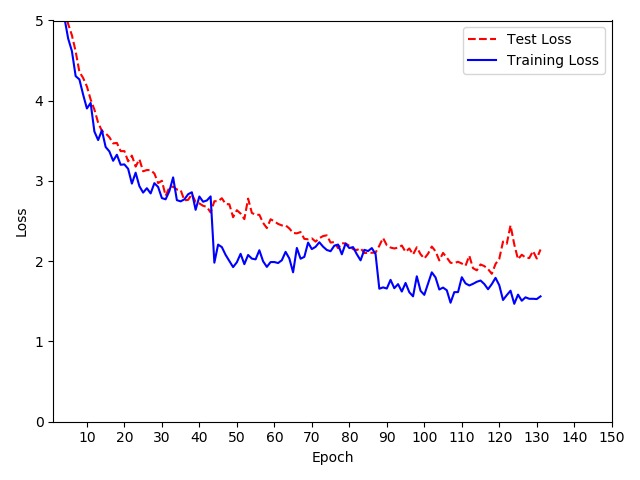
\includegraphics[width=8cm]{Bilder/ssdloss.jpeg} 
		\caption{Entwicklung der SSD Trainings- und Testverlustkurve während dem Training}
		\label{ssdloss}
	\end{center}
\end{figure}

Die Entscheidung zum \textit{Early Stopping} basiert auf dem Anstieg der Differenz zwischen Trainings- und Testverlustkurve ab Epoche 122, was auf \textit{Overfitting} schließen lässt. Zur Epoche davor war die Differenz der beiden Kurven am niedrigsten bei vergleichsweise geringem Verlust im Trainingsverfahren. Auffällig ist ebenfalls der große Abfall der Trainingsverlustkurve bei Epoche 45 und Epoche 89. Hier findet ein Wechsel im Kreuzvalidierungsverfahren statt. Die bessere Generalisierungsfähigkeit des Modells bei neuen Testdaten zeigt Ausschlag, indem die Klassifikationsergebnisse schlagartig besser werden und zu niedrigeren Kosten führen. Auch in Epoche 67 ist einer dieser Ausschläge zu sehen, der allerdings kleiner im Vergleich zu den anderen ausfällt. 

Zur Epoche 121 betrug das Ergebnis der Kostenfunktion 1.7. Es ergab eine \textit{mAP} von 83.1\%, leicht über den Referenzergebnissen von \textit{SSD} zu \textit{PascalVOC} (siehe Abbildung \ref{result}). Die Ergebnisse zu den einzelnen Klassen sind in folgender Tabelle dargestellt:

\begin{center}
	\begin{tabular}[H]{l|c}
		Klasse & mAP \\
		\hline
		Saskia Wasser Groß & 77.62\% \\
		Saskia Wasser Klein & 75.96\% \\
		Pepsi Cola Groß & 94.94\% \\
		Pepsi Cola Klein & 86.38\% \\
		ISO & 86.37\% \\
		ACE & 85.43\% \\
		Stenger Johannisbeerschorle & 69.47\% \\
		Stenger Apfelsaftschorle & 82.48 \% \\
		Vitamalz Malzbier & 76.24\%
	\end{tabular}
	\captionof{table}{Validierungsergebnisse SSD}
	\label{table:ssdresults}
\end{center}

Wird nun das trainierte Modell auf echte Daten angewendet, so fällt auf, dass manche Objekte doppelt detektiert werden. Um dieses Problem zu lösen, gibt es zwei Möglichkeiten. 

Als erstes kann bei der Detektion der minimale \textit{confidence score} angegeben werden, ab wann eine Detektion offiziell als solche wahrgenommen wird. Hier liegt die Herausforderung darin, einen optimalen Wert zu finden, sodass verdeckte Objekte noch als solche erkannt werden, aber doppelt erkannte Objekte nicht mehr auftreten. Der \textit{confidence score} wurde nach mehrmaligem Iterieren auf 0.7 festgelegt.

Die zweite Möglichkeit besteht darin, die maximale Überlappung zweier Bounding Boxen festzulegen. Somit werden doppelte Bounding Boxen, die sich flächenmäßig über einem gewissen Grenzwert überlappen, auf eine Bounding Box reduziert. Er stellte ich sich Parameter von 0.45 als geeignet heraus. Außerdem wurden Inkonsistenzen im Detektionsverhalten festgestellt.

\begin{figure}[H]
	\centering
	\subfigure[verdeckt]{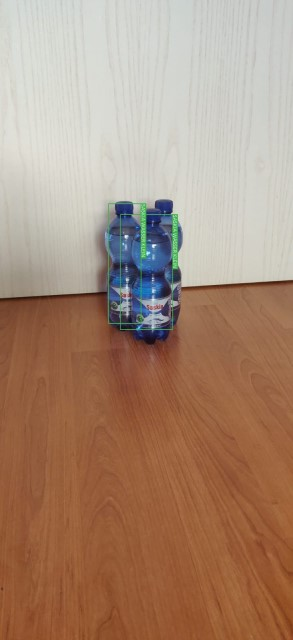
\includegraphics[width=0.30\textwidth]{Bilder/verdeckt.jpeg}}
	\hspace{2cm}
	\subfigure[winkel]{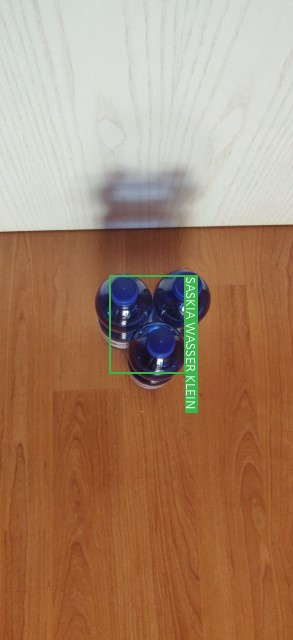
\includegraphics[width=0.30\textwidth]{Bilder/winkel.jpeg}}
	\caption{Detektionsverhalten von SSD bei extremen Blicklagen}
	\label{lagen}
\end{figure}

So sind von anderen Objekten verdeckte Objekte nur schwer zu erkennen, genauso wie Objekte aus extremen Blicklagen (siehe Abbildung \ref{lagen}). Diese Fälle wurden im Datensatz zwar zu 12.5\% abgedeckt, scheinen allerdings nur wenig Auswirkung auf besseres Detektionsverhalten für solche Fälle geliefert zu haben. Es lässt sich auch keine Aussage darüber treffen, ob eine Erweiterung des Datensatzes mit weiteren solchen Extremfällen eine Abhilfe für dieses Problem hätte liefern können. 

\begin{figure}[H]
	\subfigure[1 Meter]{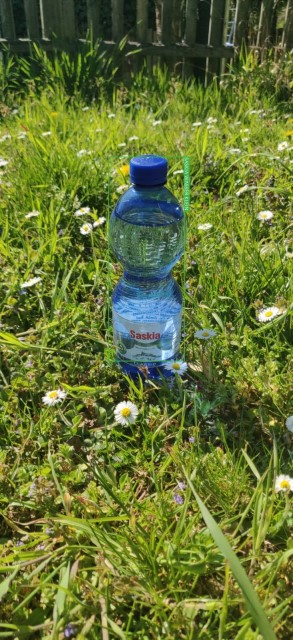
\includegraphics[width=0.30\textwidth]{Bilder/einmeter.jpeg}}\hfill
	\subfigure[2 Meter]{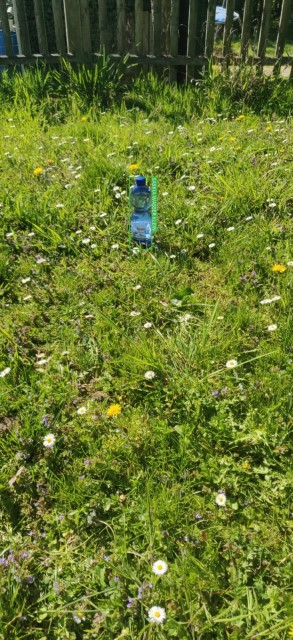
\includegraphics[width=0.30\textwidth]{Bilder/zweimeter.jpeg}}\hfill
	\subfigure[3 Meter]{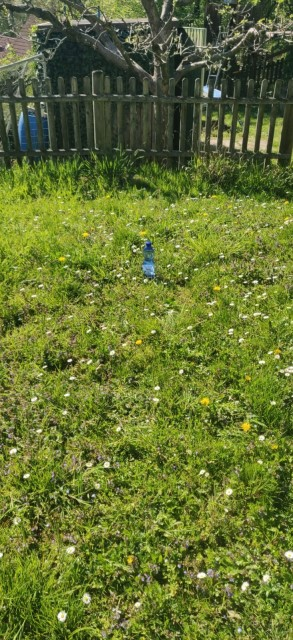
\includegraphics[width=0.30\textwidth]{Bilder/dreimeter.jpeg}}\hfill
	\caption{Detektionsverhalten von SSD bei unterschiedlichen Entfernungen}
	\label{entfernung}
\end{figure}

Auch die Entfernung zum zu detektierenden Objekt besitzt eine Auswirkung auf das Detektionsverhalten. In Abbildung \ref{entfernung} wird gezeigt, dass ab einer Entfernung von drei Metern keine Detektion mehr erfolgte. 

\begin{figure}[H]
	\subfigure[überbeleuchtet]{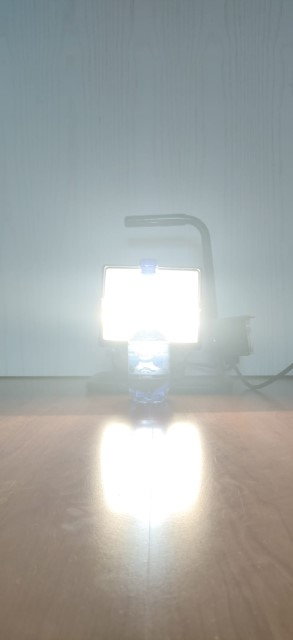
\includegraphics[width=0.30\textwidth]{Bilder/ueberbeleuchtet.jpeg}}\hfill
	\subfigure[normal]{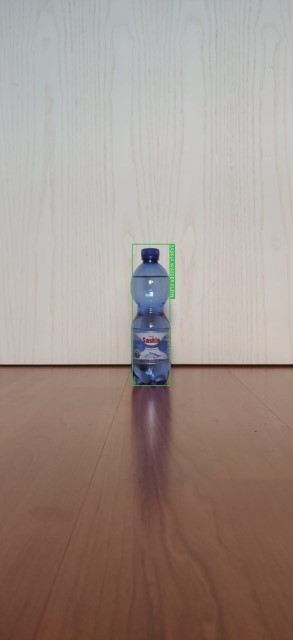
\includegraphics[width=0.30\textwidth]{Bilder/normalbeleuchtet.jpeg}}\hfill
	\subfigure[unterbeleuchtet]{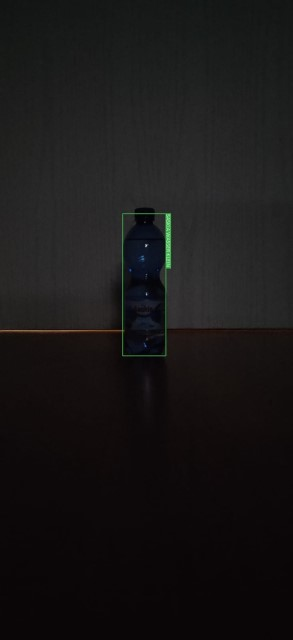
\includegraphics[width=0.30\textwidth]{Bilder/unterbeleuchtet.jpeg}}\hfill
	\caption{Detektionsverhalten von SSD bei unterschiedlichen Beleuchtungsverhältnissen}
	\label{sicht}
\end{figure}

Des Weiteren haben unterschiedliche Beleuchtungsgrade eine Auswirkung auf das Detektionsverhalten. In Abbildung \ref{sicht} wird unterschieden zwischen dem Detektionsverhalten bei überbeleuchteten, normalen und unterbeleuchteten Sichtverhältnissen. Überbeleuchtete Umgebungsverhältnisse erschweren die Objektdetektion in diesem Beispiel. 

Die Detektion reagierte allerdings invariant gegenüber unterschiedlichen Hintergründen oder Bildauflösungen.

\subsection*{YOLO}

Um eine möglichst gute Aussage über den Vergleich der beiden Objektdetektoren treffen zu können, kommt bei \textit{YOLO} der exakt gleiche Trainings- und Testdatensatz wie beim \textit{SSD} zum Einsatz. Das Training von \textit{YOLO} ergab eine \textit{mAP} von 80.36\%. Abbildung \ref{yolo_result} zeigt die Verbesserung des Modells während dem Trainingsprozess. 

\begin{figure}[H]
	\begin{center}
		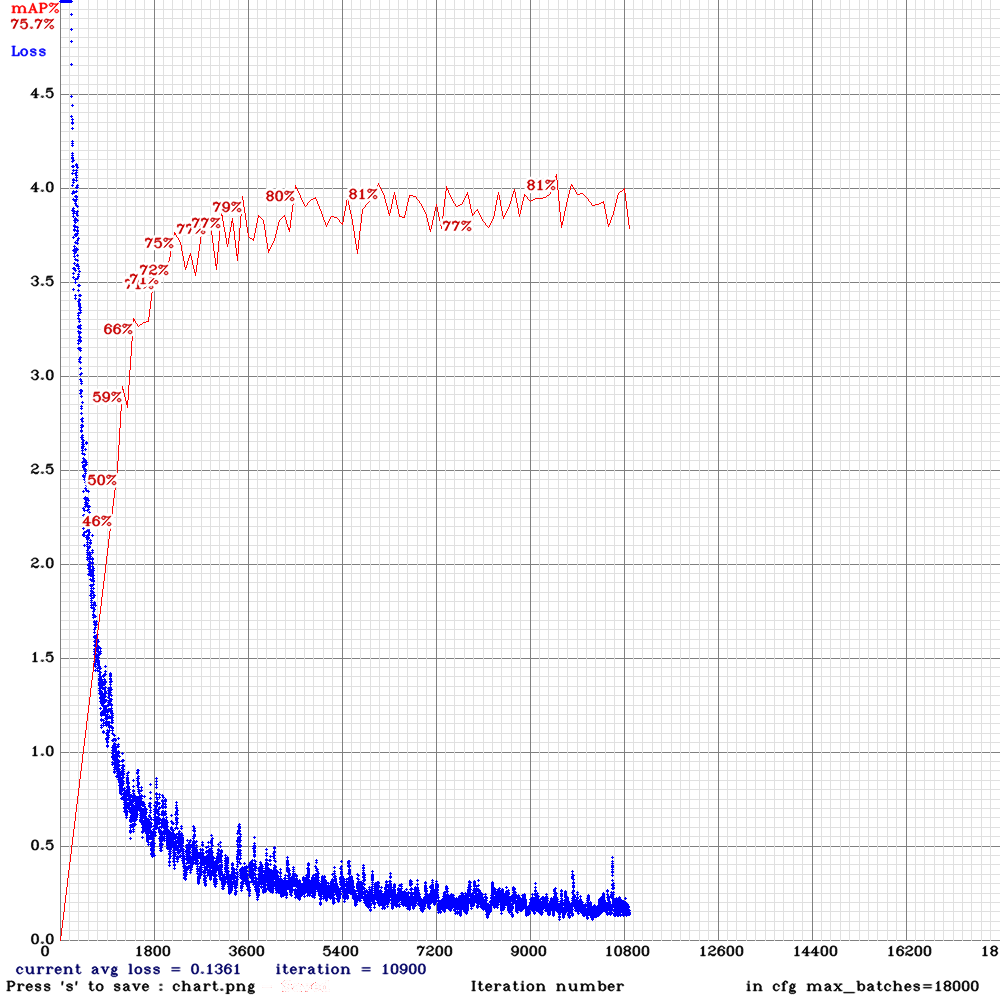
\includegraphics[width=8cm]{Bilder/yolo_result.png} 
		\caption{Entwicklung der YOLO Testverlustkurve und der \textit{mAP} während dem Training}
		\label{yolo_result}
	\end{center}
\end{figure}

Wie beim \textit{SSD} erreicht das Modell nach bereits etwa 4500 Batches eine \textit{mAP} von 80\%. Da sich das Modell ab diesem Zeitpunkt nicht mehr maßgeblich verbessert hat, wurde das Training vor Erreichung der durch die Dokumentation nahegelegte maximale Anzahl an Batches abgebrochen. Das frühe Erreichen eines sehr guten Ergebnis kann darauf zurückgeführt werden, dass es sich bei den gelabelten Klassen um Objekte des gleichen Typs handelt und das Modell dementsprechend leichter trainiert werden kann. 

Der \textit{confidence score} liegt standardmäßig bei 0.25. Nach mehreren Durchläufen stellt sich heraus, dass dieser Wert nicht verändert werden sollte. Ein zu geringer Wert sorgt zwar dafür, dass möglicherweise mehr Objekte erkannt werden, allerdings steigt damit auch die Rate an falsch oder doppelt erkannter Objekte. Ein Parameter für die Obergrenze der Überlappung zweier Bounding Boxen existiert nicht.

Tabelle \ref{table:yoloresults} zeigt die \textit{mAP} für jede Klasse.

\begin{center}
	\begin{tabular}[H]{l|c|c}
		Klasse & mAP & Differenz zu SSD\\
		\hline
		Saskia Wasser Groß & 76.69\% & (-0.93\%) \\
		Saskia Wasser Klein & 80.63\% & (+4.67\%) \\
		Pepsi Cola Groß & 73.14\% & (-21.8\%) \\
		Pepsi Cola Klein & 75.24\% & (-11.14\%) \\
		ISO & 90.28\% & (+3.91\%) \\
		ACE & 86.69\% & (+1.26\%) \\
		Stenger Johannisbeerschorle & 72.50\% & (+3.03\%) \\
		Stenger Apfelsaftschorle & 78.05\% & (-4.43\%) \\
		Vitamalz Malzbier & 81.94\% & (+5.7\%)
	\end{tabular}
	\captionof{table}{Validierungsergebnisse YOLO im Vergleich zu SSD}
	\label{table:yoloresults}
\end{center}

Auch bei \textit{YOLO} können verdeckte Objekte nur schwer erkannt werden. Ein Unterschied zu \textit{SSD} zeigt sich bei der Ansicht von oben:

\begin{figure}[H]
	\centering
	\subfigure[verdeckt]{\includegraphics[width=0.30\textwidth]{Bilder/yolo_verdeckt.jpg}}
	\hspace{2cm}
	\subfigure[winkel]{\includegraphics[width=0.30\textwidth]{Bilder/yolo_winkel.jpg}}
	\caption{Detektionsverhalten von YOLO bei extremen Blicklagen}
	\label{lagen_yolo}
\end{figure}

Hier werden zwei von drei Flaschen erkannt, die allerdings der falschen Klasse (\textit{Saskia Wasser Groß} statt \textit{Saskia Wasser Klein}) zugeordnet werden und eine der zwei Bounding Boxes zwei Flaschen umschließt.

\begin{figure}[H]
	\subfigure[1 Meter]{\includegraphics[width=0.30\textwidth]{Bilder/yolo_entfernung1.jpg}}\hfill
	\subfigure[2 Meter]{\includegraphics[width=0.30\textwidth]{Bilder/yolo_entfernung2.jpg}}\hfill
	\subfigure[3 Meter]{\includegraphics[width=0.30\textwidth]{Bilder/yolo_entfernung3.jpg}}\hfill
	\caption{Detektionsverhalten von YOLO bei unterschiedlichen Entfernungen}
	\label{entfernung_yolo}
\end{figure}

Wie bei \textit{SSD} erfolgt nach bereits drei Metern Entfernung keine Detektion mehr (siehe Abbildung \ref{entfernung_yolo}). Der \textit{confidence score} für die korrekt erkannte Bounding Box liegt bei nur 2\%.
 
\begin{figure}[H]
 	\subfigure[überbeleuchtet]{\includegraphics[width=0.30\textwidth]{Bilder/yolo_beleuchtung2.jpg}}\hfill
 	\subfigure[normal]{\includegraphics[width=0.30\textwidth]{Bilder/yolo_beleuchtung1.jpg}}\hfill
 	\subfigure[unterbeleuchtet]{\includegraphics[width=0.30\textwidth]{Bilder/yolo_beleuchtung3.jpg}}\hfill
 	\caption{Detektionsverhalten von YOLO bei unterschiedlichen Beleuchtungsverhältnissen}
 	\label{sicht_yolo}
\end{figure}

Beim Testen der verschiedenen Beleuchtungsverhältnisse fällt auf, dass im Gegensatz zum \textit{SSD} die Flasche in der unterbelichteten Umgebung nicht erkannt wird beziehungsweise mit einem \textit{confidence score} von nur 6\%. 

Gleich zu \textit{SSD} reagiert \textit{YOLO} auch invariant gegenüber unterschiedlichen Hintergründen oder Bildauflösungen.
 
\section{Reaktionsvermögen}

Bei der Inferenz fällt allerdings entgegen der Erwartungen auf, dass die Inferenz überdurchschnittlich langsam verläuft. Das Problem lässt sich auf die synchrone Arbeitsweise der bisherigen Detektionsalgorithmen zurück führen, bei dem erst ein neuer Frame des Videostreams angefragt wird, sobald das aktuelle Bild durch die Vorverarbeitung gelaufen ist und durch das Modell inferiert wurde. 

Um dem entgegen zu wirken, wurde ein Bufferkonzept in einem parallelem Thread realisiert, der einzelne Frames zeitgleich zur Inferenz anfragt und zwischenspeichert. Ist der Buffer voll, so werden nach dem \textit{First In First Out} Verfahren die älteren Frames verworfen. Dadurch konnte die FPS Anzahl von \textit{SSD} von maximal 18 auf die vollen 30 und bei \textit{YOLO} von 20 auf 28 gesteigert werden. Dadurch sollten sämtliche Änderungen in der Umgebung rechtzeitig vom Objektdetektor erkannt werden. 

Ein weiteres Problem beschreibt die initiale Latenz zwischen der Inferenz und der Bildaufnahme. Die Inferenz kann erst gestartet werden, sobald die Gewichtungen des Modells initialisiert und geladen wurden. Bei \textit{YOLO} benötigt die Initialisierung etwa drei Sekunden, bei \textit{SSD} vier Sekunden. Das lässt sich umgehen, indem entweder der Thread zur Bildaufnahme verzögern gestartet wird oder dessen Buffer kleiner gewählt wird.

\section{Trainingsverhalten}

\begin{center}
	\begin{tabular}[H]{l|c|c|c|c}
		Detektor & Hardware & Batch Größe & Dauer Epoche & Dauer Insgesamt \\
		\hline
		SSD & GTX 1080 & 16 & 9 Min. & 16.5 Std. \\
		YOLO & RTX 2060 & 64 & 1.5 Min. & 8 Std.
	\end{tabular}
	\captionof{table}{Trainingsverhalten von SSD und YOLO}
	\label{table:duration}
\end{center}

Tabelle \ref{table:duration} zeigt die Ergebnisse des Trainingsverhaltens von \textit{SSD} und \textit{YOLO}. Pro Epoche wurden 998 Bilder durchlaufen. Die Dauer der beiden Trainingsdurchläufe lässt sich allerdings nur schwer vergleichen. Zum einen wird für das Training von \textit{YOLO} eine andere GPU verwendet, deren Tensor Kerne den Trainingsprozess merklich beschleunigen. Zum anderen werden die beiden Objektdetektoren in zwei verschiedenen Frameworks implementiert, wodurch ein anderes Trainingsverhalten von Grund auf gegeben ist und Unterschiede in der Performance auftreten können. Auch die Batch Größe wurde unterschiedlich gewählt, was sich auf die Häufigkeit des Gradientenabstiegs auswirkt. Bei beiden Verfahren kann das Training durch die Ablage von sogenannten Modell-Checkpoints zu einem späteren Zeitpunkt fortgeführt werden. Das ist vor allem dann von Vorteil, wenn nachträglich Parameter oder Trainingsdaten angepasst werden und kein kompletter Neustart des Trainings erforderlich ist.


\chapter{Bewertung}

\begin{itemize}
	\item Ergebnisse bewerten und diskutieren
	\item Was liefert die Arbeit, was bisher noch nicht bekannt war (Mehrwert, auch wenn etwas nicht geht)?
\end{itemize}


\chapter{Zusammenfassung und Ausblick}

Ziel der Arbeit war es zum einen zu evaluieren, wie gut die bestehenden Objektdetektoren für industrielle Anwendungsszenarien grundsätzlich geeignet sind, zum anderen, ob das spezifische Anwendungsszenario zur Durchführung einer Inventur von Warenhäusern mit einer Drohne prototypisch umsetzbar ist. Nach dieser Arbeit sind nun folgende Erkenntnisse festzuhalten.

Zunächst ist evaluiert worden, dass Objektdetektoren wie \textit{SSD} und \textit{YOLO} durchaus das Potential ausweisen, industriell genutzt zu werden. Nicht nur hinsichtlich ihrer Präzision im Detektionsvermögen weisen sie zuversichtliche Ergebnisse auf, sondern auch in der Schnelligkeit ihrer Detektion. Beide weisen bei speziellen Detektionsszenarien ihre Stärken und Schwächen auf. Gerade die Detektion von teilweise verdeckten Objekten stellt nach wie vor ein Problem dar, für das alternative Lösungswege gefunden werden müssen. 

Daneben stellt sich die Machbarkeitsstudie \textit{Smart Warehouse} basierend auf den gegebenen Rahmenbedingungen und den getroffenen Entscheidungen als nicht machbar heraus. Es wurde eine Drohne programmiert, die ein Miniaturmodell eines Warenhauses durchfliegt. Ihr Drohnenstream konnte zwar abgefragt werden, allerdings wegen Kompatibilitätsproblemen der Laufzeitumgebungen nicht durch ein \textit{Deep Learning} Modell inferiert werden. Anstelle eines Video-Streams der Drohne wurde ein Video-Stream einer Webcam an einen Server zur Inferenz mit dem \textit{YOLO} Objektdetektionsmodell gesendet und die daraus resultierenden Objekte gezählt. Das Ergebnis und der Live-Stream der Inferenz wurden auf einer Webapplikation dargestellt. Offen bleibt das Problem einer doppelten Detektion von Objekten bei mehrfachen Erscheinen im Bild nach gewissen zeitlichen Abständen, da keine eindeutige Identifizierung von Objekten mit reiner Objektdetektion möglich ist. Damit wäre das Zählen von gleichen Objekten an unterschiedlichen Lagerplätzen mit Hilfe eines Objektdetektors nicht umsetzbar, zumindest nicht ohne weitere Zuhilfenahme von zum Beispiel einem GPS Sensor. Auch das Detektieren von verdeckten Objekten bleibt eine weitere Problematik.

Um das \textit{Smart Warehouse} Szenario weiter auszubauen, soll als nächstes der Datensatz vom simplen Beispiel von Getränkeflaschen auf eine echte Warenhausumgebung erweitert werden. Dadurch wird ebenfalls erhofft, die Präzision des Modells weiter zu verbessern und Inkonsistenzen bei unterschiedlichen Beleuchtungsverhältnissen, extremen Blicklagen, größeren Entfernungen und unterschiedlichen Verdeckungsgraden zu beheben. Zudem muss die Flugsequenz der Drohne dahingehend optimiert werden, bei Stellen starker Verdeckungsgrade alternative Betrachtungswinkel zu wählen. 

Als nächstes muss ein eigener H.264 Decoder implementiert werden, der die neuste Python Version unterstützt und im Einklang mit den verwendeten \textit{Deep Learning} Frameworks steht. Nach diesem Schritt könnten anschließend auch Live-Bilder des Video-Streams der Drohne inferiert werden.

Um abschließend spezielle Rahmenbedingungen bei der Zählung durch Objektdetektion auszuschließen, könnte das Szenario ebenso zur eindeutigen Identifizierung von Objekten mit konventionellen RFID Chips erweitert werden. Dies ermöglicht ebenso neue Szenarien zu entwickeln, in denen Objektdetektion nur Suche von Objekten einer bestimmten Klasse genutzt wird und deren Identität anschließend mit RFID Chips sichergestellt wird. 

Bei Berücksichtigung dieser Verbesserungsvorschläge, lässt sich somit durchaus auf eine Umsetzbarkeit des \textit{Smart Warehouse} Szenarios in der Zukunft hoffen.


% ---- Literaturverzeichnis
\cleardoublepage
\renewcommand*{\chapterpagestyle}{plain}
\pagestyle{plain}
\pagenumbering{Roman}                   % Römische Seitenzahlen
\setcounter{page}{\numexpr\value{savepage}+1}

\printbibliography[title=Literaturverzeichnis]
%\chapter*{Literaturverzeichnis}
%\addcontentsline{toc}{chapter}{Literaturverzeichnis}
%\printbibheading 
%\printbibliography[keyword=book,heading=subbibliography,title={Literaturquellen}] % Ausgabe der Literaturquellen
%\printbibliography[keyword=online,heading=subbibliography,title={Internetquellen}]     % Ausgabe der Internetquellen

% ---- Anhang

\newgeometry{
	left=2.5cm,
	right=2.5cm,
	top=0cm,
	bottom=2.5cm,
	includeheadfoot
}

\appendix
\chapter{Anhang}
%\captionsetup{list=false}

\section*{Abbildungen}



\restoregeometry
\newpage

\onehalfspacing
%\include{Inhalt/12_Anhang/...}

%\clearpage
%\pagenumbering{Roman}  % römische Seitenzahlen für Anhang

\end{document}
